\PassOptionsToPackage{enable-debug,check-declarations}{expl3}
\RequirePackage{pdfmanagement-testphase}
\DeclareDocumentMetadata {  }
\ExplSyntaxOn
\pdfmanagement_add:nnn{Catalog}{Lang}{(enUS)}
\ExplSyntaxOff

% xmp metadata for pdf
% Originally used \usepackage[a-2a]{pdfx}
% \usepackage{hyperxmp} replaced it
% \RequirePackage{pdfmanagement-testphase} replaced it

\documentclass[11pt,
  english,
  a4paper,
]{article}
\usepackage{sa4ss}
\usepackage{amsmath,amssymb,array}
\usepackage{booktabs}

% From tagged-template.latex
\usepackage{lmodern}
\usepackage{ifxetex,ifluatex}
\ifnum 0\ifxetex 1\fi\ifluatex 1\fi=0 % if pdftex
  \usepackage[T1]{fontenc}
  \usepackage[utf8]{inputenc}
  \usepackage{textcomp} % provide euro and other symbols
\else % if luatex or xetex
  \usepackage{unicode-math}
  \defaultfontfeatures{Scale=MatchLowercase}
  \defaultfontfeatures[\rmfamily]{Ligatures=TeX,Scale=1}
\fi

% Use upquote if available, for straight quotes in verbatim environments
\IfFileExists{upquote.sty}{\usepackage{upquote}}{}
\IfFileExists{microtype.sty}{% use microtype if available
  \usepackage[]{microtype}
  \UseMicrotypeSet[protrusion]{basicmath} % disable protrusion for tt fonts
}{}
\makeatletter
\@ifundefined{KOMAClassName}{% if non-KOMA class
  \IfFileExists{parskip.sty}{%
    \usepackage{parskip}
  }{% else
    \setlength{\parindent}{0pt}
    \setlength{\parskip}{6pt plus 2pt minus 1pt}}
}{% if KOMA class
  \KOMAoptions{parskip=half}}
\makeatother
\usepackage{xcolor}
\IfFileExists{xurl.sty}{\usepackage{xurl}}{} % add URL line breaks if available
\hypersetup{
  pdftitle={The status of Vermilion Rockfish (Sebastes miniatus) and Sunset Rockfish (Sebastes crocotulus) in U.S. waters off the coast of California north of Pt. Conception in 2021},
  pdflang={en},
  hidelinks,
  pdfcreator={LaTeX via pandoc}}
\urlstyle{same} % disable monospaced font for URLs
\usepackage{longtable}
% Correct order of tables after \paragraph or \subparagraph
\usepackage{etoolbox}
\makeatletter
\patchcmd\longtable{\par}{\if@noskipsec\mbox{}\fi\par}{}{}
\makeatother
% Allow footnotes in longtable head/foot
\IfFileExists{footnotehyper.sty}{\usepackage{footnotehyper}}{\usepackage{footnote}}
\makesavenoteenv{longtable}
\usepackage{graphicx}
\makeatletter
\def\maxwidth{\ifdim\Gin@nat@width>\linewidth\linewidth\else\Gin@nat@width\fi}
\def\maxheight{\ifdim\Gin@nat@height>\textheight\textheight\else\Gin@nat@height\fi}
\makeatother
% Scale images if necessary, so that they will not overflow the page
% margins by default, and it is still possible to overwrite the defaults
% using explicit options in \includegraphics[width, height, ...]{}
\setkeys{Gin}{width=\maxwidth,height=\maxheight,keepaspectratio}
% Set default figure placement to htbp
\makeatletter
\def\fps@figure{htbp}
\makeatother
\setlength{\emergencystretch}{3em} % prevent overfull lines
\providecommand{\tightlist}{%
  \setlength{\itemsep}{0pt}\setlength{\parskip}{0pt}}
\setcounter{secnumdepth}{5}
\usepackage{booktabs}
\usepackage{longtable}
\usepackage{array}
\usepackage{multirow}
\usepackage{wrapfig}
\usepackage{float}
\usepackage{colortbl}
\usepackage{pdflscape}
\usepackage{tabu}
\usepackage{threeparttable}
\usepackage[normalem]{ulem}
\usepackage{makecell}
\usepackage{xcolor}
\usepackage{placeins}
\ifxetex
  % Load polyglossia as late as possible: uses bidi with RTL langages (e.g. Hebrew, Arabic)
  \usepackage{polyglossia}
  \setmainlanguage[]{english}
\else
  \usepackage[shorthands=off,main=english]{babel}
\fi

%Define cslreferences environment, required by pandoc 2.8
%https://github.com/rstudio/rmarkdown/issues/1649
\newlength{\csllabelwidth}
\setlength{\csllabelwidth}{3em}
\newlength{\cslhangindent}
\setlength{\cslhangindent}{1.5em}
% for Pandoc 2.8 to 2.10.1
\newenvironment{cslreferences}%
  {}%
  {\par}
% For Pandoc 2.11+
\newenvironment{CSLReferences}[2] % #1 hanging-ident, #2 entry spacing
 {% don't indent paragraphs
  \setlength{\parindent}{0pt}
  % turn on hanging indent if param 1 is 1
  \ifodd #1 \everypar{\setlength{\hangindent}{\cslhangindent}}\ignorespaces\fi
  % set entry spacing
  \ifnum #2 > 0
  \setlength{\parskip}{#2\baselineskip}
  \fi
 }%
 {}
\usepackage{calc}  % for \widthof, \maxof in minipage
\newcommand{\CSLBlock}[1]{#1\hfill\break}
\newcommand{\CSLLeftMargin}[1]{\parbox[t]{\csllabelwidth}{#1}}
\newcommand{\CSLRightInline}[1]{\parbox[t]{\linewidth - \csllabelwidth}{#1}\break}
\newcommand{\CSLIndent}[1]{\hspace{\cslhangindent}#1}


\providecommand{\tightlist}{%
  \setlength{\itemsep}{0pt}\setlength{\parskip}{0pt}}

\usepackage{booktabs}
\usepackage{longtable}
\usepackage{array}
\usepackage{multirow}
\usepackage{wrapfig}
\usepackage{float}
\usepackage{colortbl}
\usepackage{pdflscape}
\usepackage{tabu}
\usepackage{threeparttable}
\usepackage[normalem]{ulem}
\usepackage{makecell}
\usepackage{xcolor}
\usepackage{placeins}
\date{}
\newcommand{\trTitle}{The status of Vermilion Rockfish (\emph{Sebastes miniatus}) and Sunset Rockfish (\emph{Sebastes crocotulus}) in U.S. waters off the coast of California north of Pt. Conception in 2021}
\newcommand{\trYear}{2021}
\newcommand{\trMonth}{June}
\newcommand{\trAuthsLong}{truetruetruetrue}
\newcommand{\trAuthsBack}{Monk, M.H., E.J. Dick, J.C. Field, E.M. Saas}
\newcommand{\trCitation}{
\begin{hangparas}{1em}{1}
\trAuthsBack{}. \trYear{}. \trTitle{}. Pacific Fisheries Management Council, Portland, Oregon. \pageref{LastPage}{}\,p.
\end{hangparas}}

\AtBeginDocument{\tagstructbegin{tag=Document}}
\AtEndDocument{\tagstructend}
\pretocmd{\maketitle}{\tagstructbegin{tag=H1}\tagmcbegin{tag=H1}}{}{}
\apptocmd{\maketitle}{\tagmcend\tagstructend}{}{}

\begin{document}

%%%%% Frontmatter %%%%%

% Footnote symbols in front matter
\renewcommand*{\thefootnote}{\fnsymbol{footnote}}

\small
\thispagestyle{empty}
\pagenumbering{roman}
\noindent
\begin{center}
\title{The status of Vermilion Rockfish (\emph{Sebastes miniatus}) and Sunset Rockfish (\emph{Sebastes crocotulus}) in U.S. waters off the coast of California north of Pt. Conception in 2021}
% \textnormal{\MakeTextUppercase{\trTitle{}}}
\vspace{1.5cm}
{\Large\textbf\newline{The status of Vermilion Rockfish (\emph{Sebastes miniatus}) and Sunset Rockfish (\emph{Sebastes crocotulus}) in U.S. waters off the coast of California north of Pt. Conception in 2021}}
\vfill
by\\
Melissa H. Monk\textsuperscript{1}\\
E. J. Dick\textsuperscript{1}\\
John C. Field\textsuperscript{1}\\
Emma M. Saas\textsuperscript{1}\vfill
\textsuperscript{1}Southwest Fisheries Science Center, U.S. Department of Commerce, National Oceanic and Atmospheric Administration, National Marine Fisheries Service, 110 McAllister Way, Santa Cruz, California 95060\vfill
\trMonth{} \trYear{}
\end{center}
\clearpage

% Fourth page: Colophon
\thispagestyle{empty}
\vspace*{\fill}
\begin{center}
\copyright{} Pacific Fisheries Management Council, \trYear{}\\
\end{center}
\par
\bigskip
\noindent
Correct citation for this publication:
\bigskip
\par
\trCitation{}
\clearpage

% Add TOC to pdf bookmarks (clickable pdf)
\pdfbookmark[1]{\contentsname}{toc}

% Table of contents page, lists of figures and tables
\tableofcontents\clearpage
\label{TRlastRoman}
\clearpage

% Table of contents
\newpage
\thispagestyle{empty} % to remove page number

% Settings for the main document
\pagenumbering{arabic}  % Regular page numbers
\pagestyle{plain}  % No page number on first page of main document, use 'empty'
\renewcommand*{\thefootnote}{\arabic{footnote}}  % Back to numeric footnotes
\setcounter{footnote}{0}  % And start at 1
\renewcommand{\headrulewidth}{0.5pt}
\renewcommand{\footrulewidth}{0.5pt}
%\pagestyle{fancy}\fancyhead[c]{Draft: Do not cite or circulate}

\newcommand{\lt}{\ensuremath <}
\newcommand{\gt}{\ensuremath >}

\newcommand\CapeM{$40^\circ 10^\prime N$}
\newcommand\PtC{$34^\circ 27^\prime N$}
\newcommand\CAOR{$42^\circ 00^\prime N$}

\pagebreak
\pagenumbering{roman}
\setcounter{page}{1}

\renewcommand{\thetable}{\roman{table}}
\renewcommand{\thefigure}{\roman{figure}}

\setlength\parskip{0.5em plus 0.1em minus 0.2em}

\tagstructbegin{tag=H1}\tagmcbegin{tag=H1}

\hypertarget{executive-summary}{%
\section*{Executive Summary}\label{executive-summary}}
\addcontentsline{toc}{section}{Executive Summary}

\leavevmode\tagmcend\tagstructend

To be completed after the STAR panel.

\tagstructbegin{tag=H2}\tagmcbegin{tag=H2}

\hypertarget{stock}{%
\subsection*{Stock}\label{stock}}
\addcontentsline{toc}{subsection}{Stock}

\leavevmode\tagmcend\tagstructend

This assessment reports the status of the vermlion rockfish (\emph{Sebastes miniatus}) and sunset rockfish (\emph{Sebastes crocotulus}) complex (referred to as vermilion throughout), resource in U.S. waters off the coast of California north of Point Conception ({\tagstructbegin{tag=Formula}\tagmcbegin{tag=Formula}\(34^\circ 27^\prime\)\leavevmode\tagmcend\tagstructend} N. latitude) using data through 2020.

\tagstructbegin{tag=H2}\tagmcbegin{tag=H2}

\hypertarget{landings}{%
\subsection*{Landings}\label{landings}}
\addcontentsline{toc}{subsection}{Landings}

\leavevmode\tagmcend\tagstructend

Replace text.

\tagstructbegin{tag=H2}\tagmcbegin{tag=H2}

\hypertarget{data-and-assessment}{%
\subsection*{Data and Assessment}\label{data-and-assessment}}
\addcontentsline{toc}{subsection}{Data and Assessment}

\leavevmode\tagmcend\tagstructend

Replace text.

\tagstructbegin{tag=H2}\tagmcbegin{tag=H2}

\hypertarget{stock-biomass}{%
\subsection*{Stock Biomass}\label{stock-biomass}}
\addcontentsline{toc}{subsection}{Stock Biomass}

\leavevmode\tagmcend\tagstructend

Replace text.

\tagstructbegin{tag=H2}\tagmcbegin{tag=H2}

\hypertarget{recruitment}{%
\subsection*{Recruitment}\label{recruitment}}
\addcontentsline{toc}{subsection}{Recruitment}

\leavevmode\tagmcend\tagstructend

Replace text.

\tagstructbegin{tag=H2}\tagmcbegin{tag=H2}

\hypertarget{exploitation-status}{%
\subsection*{Exploitation Status}\label{exploitation-status}}
\addcontentsline{toc}{subsection}{Exploitation Status}

\leavevmode\tagmcend\tagstructend

Replace text.

\tagstructbegin{tag=H2}\tagmcbegin{tag=H2}

\hypertarget{reference-points}{%
\subsection*{Reference Points}\label{reference-points}}
\addcontentsline{toc}{subsection}{Reference Points}

\leavevmode\tagmcend\tagstructend

Replace text.

\tagstructbegin{tag=H2}\tagmcbegin{tag=H2}

\hypertarget{management-performance}{%
\subsection*{Management Performance}\label{management-performance}}
\addcontentsline{toc}{subsection}{Management Performance}

\leavevmode\tagmcend\tagstructend

Replace text.

\tagstructbegin{tag=H2}\tagmcbegin{tag=H2}

\hypertarget{unresolved-problems-and-major-uncertainties}{%
\subsection*{Unresolved Problems and Major Uncertainties}\label{unresolved-problems-and-major-uncertainties}}
\addcontentsline{toc}{subsection}{Unresolved Problems and Major Uncertainties}

\leavevmode\tagmcend\tagstructend

Replace text.

\tagstructbegin{tag=H2}\tagmcbegin{tag=H2}

\hypertarget{decision-table}{%
\subsection*{Decision Table}\label{decision-table}}
\addcontentsline{toc}{subsection}{Decision Table}

\leavevmode\tagmcend\tagstructend

Replace text.

\tagstructbegin{tag=H2}\tagmcbegin{tag=H2}

\hypertarget{research-and-data-needs}{%
\subsection*{Research and Data Needs}\label{research-and-data-needs}}
\addcontentsline{toc}{subsection}{Research and Data Needs}

\leavevmode\tagmcend\tagstructend

Replace text.

\pagebreak
\setlength{\parskip}{5mm plus1mm minus1mm}
\pagenumbering{arabic}
\setcounter{page}{1}
\renewcommand{\thefigure}{\arabic{figure}}
\renewcommand{\thetable}{\arabic{table}}
\setcounter{table}{0}
\setcounter{figure}{0}

\tagstructbegin{tag=H1}\tagmcbegin{tag=H1}

\hypertarget{introduction}{%
\section{Introduction}\label{introduction}}

\leavevmode\tagmcend\tagstructend

\tagstructbegin{tag=H2}\tagmcbegin{tag=H2}

\hypertarget{basic-information}{%
\subsection{Basic Information}\label{basic-information}}

\leavevmode\tagmcend\tagstructend

\#\#Basic Information and Life History

\emph{Population Structure and Complex Assessment Considerations}

This assessment represents the cryptic species pair vermilion rockfish (\emph{Sebastes miniatus}) and sunset rockfish (\emph{Sebastes crocotulus}). Hyde {\tagstructbegin{tag=Reference}\tagmcbegin{tag=Reference}(2007)\leavevmode\tagmcend\tagstructend} found seven mirochondrial and two nuclear genes analysis suggested three species within the subgenus \emph{Rosicola}. Hyde et al.~ {\tagstructbegin{tag=Reference}\tagmcbegin{tag=Reference}(2008)\leavevmode\tagmcend\tagstructend} described sunset rockfish as a distinct species noting depth separation of the adult populations of the two species using nine microsatellite loci. Sunset rockfish is distributed at depths greater than 50 fm (100 m) and are predominantly located south of Pt. Conception ($34^\circ 27^\prime N$). Hyde and Budrick identified speciation using mtDNA assay and size microsatelite loci, respectively. The mtDNA analyses proved to be subject to introgression and mis-specification of sunset rockfish from mating between the two species post-divergence. Additional population clusters of vermilion were found north of Pt. Conception, but neither study detected population structure between Half Moon Bay, California and Brookings, OR {\tagstructbegin{tag=Reference}\tagmcbegin{tag=Reference}(J. R. Hyde and Vetter 2009; Budrick 2016)\leavevmode\tagmcend\tagstructend}.

Vermilion and sunset rockfishes are morphologically very similar, with the most commonly cited differentiating feature being color. Hyde noted differences in three of six morphological parameters examined, but none of them can readily be used for field identification.

In all historical and current recreational and commercial catches, sunset and vermilion rockfish are both recorded as vermilion rockfish. Future studies, such as the one described below will provide data needed to compare biological parameters between the two species as well as habitats.

\emph{Ongoing Research (Provided by John Harms, NWFSC)}

A group of researchers from the NWFSC and SWFSC is collaborating on a project to genotype tissue specimens collected from the vermilion and sunset rockfish cryptic pair captured during the West Coast Groundfish Bottom Trawl Survey and the Southern CA Shelf Rockfish Hook and Line Survey for the years 2004 - 2019. Funding for this project was obtained through the Saltonstall-Kennedy program for FY 2020 through a proposal led by representatives from Pacific States Marine Fisheries Commission and the commercial passenger fishing vessel industry in southern California.

After combining with specimens obtained through other collection efforts along the West Coast, approximately 25,000 tissue specimens will be analyzed. Some earlier efforts to separate this cryptic pair to species used mitochondrial DNA (mtDNA) markers. However, due to a one-way mitochondrial introgression from the vermilion genome into the sunset genome, a portion of the sunset rockfish population contains mitochondrial DNA sequences consistent with vermilion rockfish resulting in incorrect species assignments for these introgressed individuals during the prior research project. The current research has identified a robust suite of genetic markers within the nuclear genomes of the two species that definitively separates vermilion and sunset rockfish (including introgressed sunset rockfish), canary rockfish, first generation vermilion-sunset hybrids, and identifies emerging patterns of intraspecific stock structure within the two sister species.

Once the collected specimens have been genotyped, any species-specific differences in spatial and depth distribution, size composition, weight-length relationships, and other biological characteristics will be identified. Using previously collected otoliths and ovaries, the demographics of the two species including age and growth and reproductive biology parameters such as length and age at 50\% maturity and the prevalence of skip spawning will be explored and compared. These new genotyping results will be combined with data from the prior mtDNA work to evaluate whether introgressed sunset rockfish represent a biologically intermediate subform of the species complex. The effort also proposes to develop and test the efficacy of models to predict the relative proportion of the two species based upon explanatory variables including latitude, depth, species of co-occurrence, oceanographic parameters, habitat descriptors and/or other information. The anticipated completion of the genotyping of all specimens is approximately December 2021 with provision of final results by the end of FY 2022.

This research is aimed at providing information to support the successful stock assessment of this commercially and recreationally valuable cryptic species pair and is responsive to any data gaps identified by the assessment community. If successful, this research, conducted in close communication with stock assessors, may also assist the PFMC in establishing best practices for the assessment and management of cryptic species complexes. Though this project will only focus on nominal vermilion rockfish specimens collected through the 2019 survey field season, it may be advisable that tissue specimens collected aboard fishery-independent surveys as well as through fishery-dependent programs continue to be genotyped on an ongoing basis to support continued and timely monitoring of this economically and ecologically important species complex.

\tagstructbegin{tag=H2}\tagmcbegin{tag=H2}

\hypertarget{early-life-history}{%
\subsection{Early Life History}\label{early-life-history}}

\leavevmode\tagmcend\tagstructend

Get from Emma

\#\#Map A map showing the scope of the two vermilion rockfish assessments and depicting boundaries at Point Conception ($34^\circ 27^\prime N$) that separates the two assessments. THe northern model is bounded by the California/Oregon border and the southern model is bounded by the U.S./ Mexico border at the south (Figure \ref{fig:assess-area}). Cape Mendocino ($40^\circ 10^\prime N$) is also noted as it is a management boundary for the stock.

\#\#Ecosystem Considerations

John is writing

\tagstructbegin{tag=H2}\tagmcbegin{tag=H2}

\hypertarget{historical-and-current-fishery-information}{%
\subsection{Historical and Current Fishery Information}\label{historical-and-current-fishery-information}}

\leavevmode\tagmcend\tagstructend

The hook-and-line fishery off California developed in the late 19th century {\tagstructbegin{tag=Reference}\tagmcbegin{tag=Reference}(Love, Yoklavich, and Thorsteinson 2002)\leavevmode\tagmcend\tagstructend}. The rockfish trawl fishery was established in the early 1940s, when the United States became involved in World War II and wartime shortage of red meat created an increased demand for other sources of protein {\tagstructbegin{tag=Reference}\tagmcbegin{tag=Reference}(Alverson, Pruter, and Ronholt 1964; Harry and Morgan 1961)\leavevmode\tagmcend\tagstructend}.

Remainder from E.J.?

\tagstructbegin{tag=H2}\tagmcbegin{tag=H2}

\hypertarget{summary-of-management-history}{%
\subsection{Summary of Management History}\label{summary-of-management-history}}

\leavevmode\tagmcend\tagstructend

Prior to the adoption of the Pacific Coast Groundfish Fishery Management Plan (FMP) in 1982, vermilion rockfish were managed through a regulatory process that included the California Department of Fish and Wildlife (CDFW) along with either the California State Legislature or the Fish and Game Commission (FGC) depending on the sector (recreation or commercial) and fishery. With implementation of the Pacific Coast Groundfish FMP, vermilion rockfish came under the management authority of the Pacific Fishery Management Council (PFMC), and were managed as part of the \emph{Sebastes} complex. Because neither species had undergone rigorous stock assessment and did not compose a large fraction of the landings they were classified and managed as part of ``Remaining Rockfish'' under the larger heading of ``Other Rockfish'' (PFMC {\tagstructbegin{tag=Reference}\tagmcbegin{tag=Reference}(2004, 2002)\leavevmode\tagmcend\tagstructend}).

Since the early 1980s a number of federal regulatory measures have been used to manage the commercial rockfish fishery including cumulative trip limits (generally for two- month periods) and seasons. Starting in 1994 the commercial groundfish fishery sector was divided into two components: limited entry and open access with specific regulations designed for each component. Other regulatory actions for the general rockfish categories have included area closures, gear restrictions, and cumulative bimonthly trip limits set for the four different commercial sectors - limited entry fixed gear, limited entry trawl, open access trawl, and open access non-trawl. Harvest guidelines are also used to regulate the annual harvest for both the recreational and commercial sectors.

In 2000, changes in the PFMC's rockfish management structure resulted in the discontinued use of the \emph{Sebastes} complex, and was replaced with three species groups: nearshore, shelf, and slope rockfishes (January 4, 2000; 65 FR 221), of which vermilion rockfish are included in the minor shelf rockfish group.

During the late 1990s and early 2000s, major changes also occurred in the way that California managed its nearshore fishery. The Marine Life Management Act (MLMA), which was passed in 1998 by the California Legislature and enacted in 1999, required that the FGC adopt an FMP for nearshore finfish {\tagstructbegin{tag=Reference}\tagmcbegin{tag=Reference}(Wilson-Vandenberg, Larinto, and Key 2014)\leavevmode\tagmcend\tagstructend}.

Following adoption of the Nearshore FMP and accompanying regulations by the FGC in fall of 2002, the FGC adopted regulations in November 2002 which established a set of marine reserves around the Channel Islands in southern California (which became effective April 2003). The FGC also adopted a nearshore restricted access program in December 2002 (which included the establishment of a Deeper Nearshore Permit) to be effective starting in the 2003 fishing year.

Also, since the enactment of the MLMA, the Council and State in a coordinated effort developed and adopted various management specifications to keep harvest within the harvest targets, including seasonal and area closures (e.g.~the CCAs; a closure of Cordell Banks to specific fishing), depth restrictions, minimum size limits, and bag limits to regulate the recreational fishery and license and permit regulations, finfish trap permits, gear restrictions, seasonal and area closures (e.g.~the RCAs and CCAs; a closure of Cordell Banks to specific fishing), depth restrictions, trip limits, and minimum size limits to regulate the commercial fishery.

The state of California has adopted regulatory measures to manage the minor seashore shallow rockfish fishery based on the harvest guidelines set forth by the PFMC. The commercial open access and limited entry fixed gear sectors have undergone three different spatial management changes since 2000. Since 2005, both have managed the area south of $40^\circ 10^\prime N$ as one area. The open access commercial fishery is managed based on bimonthly allowable catches, that have ranged from 200 pounds to 1800 pounds per two months since 2000. From 2005 to 2018, the catch limits have doubled and are now set at 1200 pounds per two months (for all months) with March and April remaining closed. The limited entry fixed gear sector has followed the same pattern as the open access sector with bi-monthly limits and a doubling of the catch since 2005. The limited entry trawl fleet is managed on monthly limits on an annual basis. Since 2011, the limit has been 300 pounds per month for non-IFQ species. A history of California's commercial regulations from 2000-2018 can be found in {\tagstructbegin{tag=Link}\tagmcbegin{tag=Link}\protect\hyperlink{appendix-a.-californias-commercial-fishery-regulations}{Appendix A}\leavevmode\tagmcend\tagstructend}. A 10-inch total length minimum size limit was implemented in 1999 for both species in the commercial fleet.

\textbf{Recreational Fisheries}

Significant regulatory changes in California's recreational sector began with a change from unlimited number of hooks and lines allowed prior to 2000 to no more than three hooks and one line per angler in 2000. Since 2001, the limit has been no more than two hooks and one line per angler. There is no size limit in the recreational fishery for vermilion rockfish. A nearshore complex sub-bag limit that included vermilion rockfish was in place from 1999 to 2005, but was eliminated thereafter.

California also began spatial management, including area closures, and depth restrictions for the recreational fleet in 2000. In general, the recreational season north of Point Conception extends from April to December, and south of Point Conception from March to December. In the area that vermilion rockfish are most commonly landed, from Monterey to Morro Bay, the maximum depth open to recreational fishing has been between 30 and 40 fathoms until 2017. In 2017 the depth restrictions were eased by 10 fathoms, opening up fishing depths along the central California coast that had not been open consistently since 2002. In both 2017 and 2018, the deepest 10 fathoms was closed prior to the prescribed season in December due to high by-catch rates of yelloweye rockfish, one of two rockfish species that are still overfished. A full history of the recreational regulations relating to the spatial management of the fleet can be found frog. Beginning on January 1, 2021 CDFW implemented a five-fish sub-bag limit for vermilion rockfish that is not accounted for in this stock assessment.

\textbf{Cowcod Conservation Areas (CCA)} In 2001, two area closures {\tagstructbegin{tag=Link}\tagmcbegin{tag=Link}\href{https://nrm.dfg.ca.gov/FileHandler.ashx?DocumentID=36132\&inline}{``Cowcod Conservation Areas''}\leavevmode\tagmcend\tagstructend} were implemented to reduce fishing mortality of cowcod, originally prohibiting bottom-fishing deeper than 20 fm. Effective 2019, retention of nearshore and shelf rockfish (excluding cowcod) is allowed in depths shallower than 40 fm. The larger of the two areas (CCA West) is a 4200 square mile area west of Santa Catalina and San Clemente Islands. A smaller area (CCA East) is about 40 miles offshore of San Diego, and covers about 100 square miles.

\textbf{Rockfish Conservation Areas (RCA)} In 2002 the PFMC established trawl- and non-trawl area closures known as the Rockfish Conservation Areas. These closed areas are gear-specific, and have seasonally changing boundaries to help reduce fishing mortality.

\tagstructbegin{tag=H2}\tagmcbegin{tag=H2}

\hypertarget{management-performance-1}{%
\subsection{Management Performance}\label{management-performance-1}}

\leavevmode\tagmcend\tagstructend

The contribution of vermilion rockfish to the shelf rockfish OFLs is currently derived from the data-poor Depletion Corrected Average Catch model {\tagstructbegin{tag=Reference}\tagmcbegin{tag=Reference}(Dick and MacCall 1994)\leavevmode\tagmcend\tagstructend}. A 2005 assessment was not accepted for management and a 2013 data-moderate assessment was not reviewed by the STAR panel due to insufficient time.

Total mortality for vermilion rockfish was obtaid from the Groundfish Expanded Mortality Multiyear {\tagstructbegin{tag=Link}\tagmcbegin{tag=Link}\href{https://www.nwfsc.noaa.gov/data/api/v1/source/observer.gemm_fact/selection.xlsx}{GEMM}\leavevmode\tagmcend\tagstructend} report {\tagstructbegin{tag=Reference}\tagmcbegin{tag=Reference}(Somers et al. 2020)\leavevmode\tagmcend\tagstructend}. The coastwide management of the shelf rockfish complex is split at Cape Mendocino ($40^\circ 10^\prime N$). Therefore, the northern California vermilion rockfish model contains a portion of the management area from Cape Mendocino ($40^\circ 10^\prime N$) to the California-Oregon border ($42^\circ 00^\prime N$). The southern California vermilion rockfish contains the area within the southern management area (south of $40^\circ 10^\prime N$) south of Pt. Conception ($34^\circ 27^\prime N$).

The total mortality of the nearshore rockfish south complex has been above the OFL in all years (2011-2019) north of $40^\circ 10^\prime N$, and above the OFL south of $40^\circ 10^\prime N$ from 2015-2019. Total mortality estimates from the NMFS NWFSC are not yet available for 2020 (Table \ref{tab:management}). Vermilion rockfish total mortality was on average 63\% (range 59\%-69\%) of the total shelf rockfish south of $40^\circ 10^\prime N$ total mortality from 2011-2016. Vermilion rockfish decreased from 28\% to 4\% of the total contribution to the shelf rockfish complex north of $40^\circ 10^\prime N$ from 2011-2019 with a noticeable decline from 23\% to 7\% from 2016 to 2017.

\tagstructbegin{tag=H2}\tagmcbegin{tag=H2}

\hypertarget{foreign-fisheries}{%
\subsection{Foreign Fisheries}\label{foreign-fisheries}}

\leavevmode\tagmcend\tagstructend

The California assessments of vermilion rockfish do not reflect any foreign fisheries in Canada.

\emph{Sebastes} spp. are not in the Fisheries National Chart (FNC, database containing species status) maintained by the Mexican Government, i.e., they are not commercially harvested in the northwest Mexican Pacific Ocean (E.M. Bojóorquez, Centro de Investigaciones Biológicas del Noroeste, S.C., perconal communication). Dr.~Bojóorque also reached out to colleagues at the {[}Fisheries National Institute{]} ({\tagstructbegin{tag=Link}\tagmcbegin{tag=Link}\url{https://www.gob.mx/inapesca}\leavevmode\tagmcend\tagstructend}) who reported that rockfish are occasionally caught in the sport fishery in the Ensenada City.

\tagstructbegin{tag=H1}\tagmcbegin{tag=H1}

\hypertarget{data}{%
\section{Data}\label{data}}

\leavevmode\tagmcend\tagstructend

Descriptions of each data source included in the model (Figure \ref{fig:data-plot}) and sources that were explored but not included are provided below.

\tagstructbegin{tag=H2}\tagmcbegin{tag=H2}

\hypertarget{fishery-dependent-data}{%
\subsection{Fishery-Dependent data}\label{fishery-dependent-data}}

\leavevmode\tagmcend\tagstructend

\tagstructbegin{tag=H2}\tagmcbegin{tag=H2}

\hypertarget{fishery-dependent-data-1}{%
\subsection{Fishery-Dependent Data}\label{fishery-dependent-data-1}}

\leavevmode\tagmcend\tagstructend

\#\#\#Commercial Landings and Discards

\emph{Commercial Landings Prior to 1916}

For landings estimates prior to 1916, we based our reconstruction on the total rockfish catches reported in a summary of early California fisheries landings by Sette and Fielder {\tagstructbegin{tag=Reference}\tagmcbegin{tag=Reference}(1927)\leavevmode\tagmcend\tagstructend} for the years 1888, 1892, 1895, 1899, 1904, 1908 and 1915. No rockfish were reported for 1888, thus we assumed no catches for that year and interpolated the catches between 0 and the 1892 catches (total of 834 tons) reported. Similarly, catches between the reported years were interpolated assuming a straight linear trend between the years reported. We used a ratio-estimator derived from the catch reconstruction fraction of vermillion rockfish in total rockfish landings for the 1916 to 1919 period (the ratio for a comparable five year period was nearly identical). We apportioned the catches north and south of Point Conception based on ratio estimators that used the same assumptions used to apportion catches in the reconstruction time period (1916-1968). The catch reconstruction estimates indicated that vermillion made up slightly under 1\% of the total rockfish catches during the early (1916-1919) time period, although the estimates indicate a slightly larger fraction (1.5\%) of total catches south of Conception relative to the fraction of total catches to the north (0.9\%). However, it is likely that the reconstruction is overestimating the fraction of smaller and/or more deeply distributed species relative to larger, shallower species as the reconstruction is based on the species composition data collected from market category samples in the late 1970s and early 1980s. The fishery has been shown to have progressed over time from a shallower, more nearshore distribution of effort to one in which deeper and more offshore waters were targeted {\tagstructbegin{tag=Reference}\tagmcbegin{tag=Reference}(Miller et al. 2014)\leavevmode\tagmcend\tagstructend}. The notion that vermillion catches may have been greater is also consistent with the recognition by Roedel {\tagstructbegin{tag=Reference}\tagmcbegin{tag=Reference}(1948)\leavevmode\tagmcend\tagstructend} that during the 1930s and 1940s vermillion were ``One of the more important commercial species, it is one of three leading species in Southern California.'' However, by the time of that report, vermillion represented 5 to 8\% of the southern California catch (based on Ralston et al. {\tagstructbegin{tag=Reference}\tagmcbegin{tag=Reference}(2010)\leavevmode\tagmcend\tagstructend}), much more than at the beginning of the time series. Future efforts to improve historical catch reconstructions by accounting for the shift in effort over time to deeper waters should continue to be flagged as a research need.

\tagstructbegin{tag=H2}\tagmcbegin{tag=H2}

\hypertarget{fishery-dependent-data-2}{%
\subsection{Fishery-Dependent Data}\label{fishery-dependent-data-2}}

\leavevmode\tagmcend\tagstructend

\tagstructbegin{tag=H2}\tagmcbegin{tag=H2}

\hypertarget{fishery-independent-data}{%
\subsection{Fishery-Independent data}\label{fishery-independent-data}}

\leavevmode\tagmcend\tagstructend

\tagstructbegin{tag=H2}\tagmcbegin{tag=H2}

\hypertarget{fishery-dependent-data-3}{%
\subsection{Fishery-Dependent Data}\label{fishery-dependent-data-3}}

\leavevmode\tagmcend\tagstructend

\tagstructbegin{tag=H3}\tagmcbegin{tag=H3}

\hypertarget{section}{%
\subsubsection{\texorpdfstring{\acrlong{s-wcgbt}}{}}\label{section}}

\leavevmode\tagmcend\tagstructend

The \Gls{s-wcgbt} is based on a random-grid design; covering the coastal waters from a depth of 55-1,280 m {\tagstructbegin{tag=Reference}\tagmcbegin{tag=Reference}(\textbf{bradburn\_2003\_2011?})\leavevmode\tagmcend\tagstructend}. This design generally uses four industry-chartered vessels per year assigned to a roughly equal number of randomly selected grid cells and divided into two `passes' of the coast. Two vessels fish from north to south during each pass between late May to early October. This design therefore incorporates both vessel-to-vessel differences in catchability, as well as variance associated with selecting a relatively small number (approximately 700) of possible cells from a very large set of possible cells spread from the Mexican to the Canadian borders.

\tagstructbegin{tag=H3}\tagmcbegin{tag=H3}

\hypertarget{section-1}{%
\subsubsection{\texorpdfstring{\acrlong{s-ccfrp}}{}}\label{section-1}}

\leavevmode\tagmcend\tagstructend

Since 2007, the \Gls{s-ccfrp} has monitored several areas in California to evaluate the performance of \Gls{mpa}s and understand nearshore fish populations {\tagstructbegin{tag=Reference}\tagmcbegin{tag=Reference}(Wendt and Starr 2009; Starr et al. 2015)\leavevmode\tagmcend\tagstructend}. In 2017, the survey expanded beyond the four \Gls{mpa}s in central California (Año Nuevo, Point Lobos, Point Buchon, and Piedras Blancas) to include the entire California coast. Fish are collected by volunteer anglers aboard \Gls{cpfv}s guided by one of the following academic institutions based on proximity to fishing location: Humboldt State University; Bodega Marine Laboratories; Moss Landing Marine Laboratories; Cal Poly San Luis Obispo; University of California, Santa Barbara; and Scripps Institution of Oceanography.

Surveys consist of fishing with hook-and-line gear for 30-45 minutes within randomly chosen 500 by 500 m grid cells within and outside \Gls{mpa}s. Prior to 2017, all fish were measured for length and release or descended to depth; since then, some were sampled for otoliths and fin clips.

\tagstructbegin{tag=H3}\tagmcbegin{tag=H3}

\hypertarget{data-sources-considered-but-not-used}{%
\subsubsection{Data sources considered, but not used}\label{data-sources-considered-but-not-used}}

\leavevmode\tagmcend\tagstructend

\tagstructbegin{tag=H2}\tagmcbegin{tag=H2}

\hypertarget{fishery-dependent-data-4}{%
\subsection{Fishery-Dependent Data}\label{fishery-dependent-data-4}}

\leavevmode\tagmcend\tagstructend

\#\#\#Commercial Landings and Discards

\emph{Commercial Landings Prior to 1916}

For landings estimates prior to 1916, we based our reconstruction on the total rockfish catches reported in a summary of early California fisheries landings by Sette and Fielder {\tagstructbegin{tag=Reference}\tagmcbegin{tag=Reference}(1927)\leavevmode\tagmcend\tagstructend} for the years 1888, 1892, 1895, 1899, 1904, 1908 and 1915. No rockfish were reported for 1888, thus we assumed no catches for that year and interpolated the catches between 0 and the 1892 catches (total of 834 tons) reported. Similarly, catches between the reported years were interpolated assuming a straight linear trend between the years reported. We used a ratio-estimator derived from the catch reconstruction fraction of vermillion rockfish in total rockfish landings for the 1916 to 1919 period (the ratio for a comparable five year period was nearly identical). We apportioned the catches north and south of Point Conception based on ratio estimators that used the same assumptions used to apportion catches in the reconstruction time period (1916-1968). The catch reconstruction estimates indicated that vermillion made up slightly under 1\% of the total rockfish catches during the early (1916-1919) time period, although the estimates indicate a slightly larger fraction (1.5\%) of total catches south of Conception relative to the fraction of total catches to the north (0.9\%). However, it is likely that the reconstruction is overestimating the fraction of smaller and/or more deeply distributed species relative to larger, shallower species as the reconstruction is based on the species composition data collected from market category samples in the late 1970s and early 1980s. The fishery has been shown to have progressed over time from a shallower, more nearshore distribution of effort to one in which deeper and more offshore waters were targeted {\tagstructbegin{tag=Reference}\tagmcbegin{tag=Reference}(Miller et al. 2014)\leavevmode\tagmcend\tagstructend}. The notion that vermillion catches may have been greater is also consistent with the recognition by Roedel {\tagstructbegin{tag=Reference}\tagmcbegin{tag=Reference}(1948)\leavevmode\tagmcend\tagstructend} that during the 1930s and 1940s vermillion were ``One of the more important commercial species, it is one of three leading species in Southern California.'' However, by the time of that report, vermillion represented 5 to 8\% of the southern California catch (based on Ralston et al. {\tagstructbegin{tag=Reference}\tagmcbegin{tag=Reference}(2010)\leavevmode\tagmcend\tagstructend}), much more than at the beginning of the time series. Future efforts to improve historical catch reconstructions by accounting for the shift in effort over time to deeper waters should continue to be flagged as a research need.

\tagstructbegin{tag=H2}\tagmcbegin{tag=H2}

\hypertarget{fishery-dependent-data-5}{%
\subsection{Fishery-Dependent Data}\label{fishery-dependent-data-5}}

\leavevmode\tagmcend\tagstructend

\#\#\#Commercial Landings and Discards

\emph{Commercial Landings Prior to 1916}

For landings estimates prior to 1916, we based our reconstruction on the total rockfish catches reported in a summary of early California fisheries landings by Sette and Fielder {\tagstructbegin{tag=Reference}\tagmcbegin{tag=Reference}(1927)\leavevmode\tagmcend\tagstructend} for the years 1888, 1892, 1895, 1899, 1904, 1908 and 1915. No rockfish were reported for 1888, thus we assumed no catches for that year and interpolated the catches between 0 and the 1892 catches (total of 834 tons) reported. Similarly, catches between the reported years were interpolated assuming a straight linear trend between the years reported. We used a ratio-estimator derived from the catch reconstruction fraction of vermillion rockfish in total rockfish landings for the 1916 to 1919 period (the ratio for a comparable five year period was nearly identical). We apportioned the catches north and south of Point Conception based on ratio estimators that used the same assumptions used to apportion catches in the reconstruction time period (1916-1968). The catch reconstruction estimates indicated that vermillion made up slightly under 1\% of the total rockfish catches during the early (1916-1919) time period, although the estimates indicate a slightly larger fraction (1.5\%) of total catches south of Conception relative to the fraction of total catches to the north (0.9\%). However, it is likely that the reconstruction is overestimating the fraction of smaller and/or more deeply distributed species relative to larger, shallower species as the reconstruction is based on the species composition data collected from market category samples in the late 1970s and early 1980s. The fishery has been shown to have progressed over time from a shallower, more nearshore distribution of effort to one in which deeper and more offshore waters were targeted {\tagstructbegin{tag=Reference}\tagmcbegin{tag=Reference}(Miller et al. 2014)\leavevmode\tagmcend\tagstructend}. The notion that vermillion catches may have been greater is also consistent with the recognition by Roedel {\tagstructbegin{tag=Reference}\tagmcbegin{tag=Reference}(1948)\leavevmode\tagmcend\tagstructend} that during the 1930s and 1940s vermillion were ``One of the more important commercial species, it is one of three leading species in Southern California.'' However, by the time of that report, vermillion represented 5 to 8\% of the southern California catch (based on Ralston et al. {\tagstructbegin{tag=Reference}\tagmcbegin{tag=Reference}(2010)\leavevmode\tagmcend\tagstructend}), much more than at the beginning of the time series. Future efforts to improve historical catch reconstructions by accounting for the shift in effort over time to deeper waters should continue to be flagged as a research need.

\tagstructbegin{tag=H1}\tagmcbegin{tag=H1}

\hypertarget{assessment-model}{%
\section{Assessment Model}\label{assessment-model}}

\leavevmode\tagmcend\tagstructend

\tagstructbegin{tag=H2}\tagmcbegin{tag=H2}

\hypertarget{summary-of-previous-assessments-and-reviews}{%
\subsection{Summary of Previous Assessments and Reviews}\label{summary-of-previous-assessments-and-reviews}}

\leavevmode\tagmcend\tagstructend

\tagstructbegin{tag=H3}\tagmcbegin{tag=H3}

\hypertarget{history-of-modeling-approaches-not-required-for-an-update-assessment}{%
\subsubsection{History of Modeling Approaches (not required for an update assessment)}\label{history-of-modeling-approaches-not-required-for-an-update-assessment}}

\leavevmode\tagmcend\tagstructend

\tagstructbegin{tag=H3}\tagmcbegin{tag=H3}

\hypertarget{most-recent-star-panel-and-ssc-recommendations-not-required-for-an-update-assessment}{%
\subsubsection{Most Recent STAR Panel and SSC Recommendations (not required for an update assessment)}\label{most-recent-star-panel-and-ssc-recommendations-not-required-for-an-update-assessment}}

\leavevmode\tagmcend\tagstructend

\tagstructbegin{tag=H3}\tagmcbegin{tag=H3}

\hypertarget{response-to-star-panel-requests-not-required-in-draft}{%
\subsubsection{Response to STAR Panel Requests (not required in draft)}\label{response-to-star-panel-requests-not-required-in-draft}}

\leavevmode\tagmcend\tagstructend

\tagstructbegin{tag=H2}\tagmcbegin{tag=H2}

\hypertarget{model-structure-and-assumptions}{%
\subsection{Model Structure and Assumptions}\label{model-structure-and-assumptions}}

\leavevmode\tagmcend\tagstructend

\tagstructbegin{tag=H3}\tagmcbegin{tag=H3}

\hypertarget{model-changes-from-the-last-assessment-not-required-for-an-update-assessment}{%
\subsubsection{Model Changes from the Last Assessment (not required for an update assessment)}\label{model-changes-from-the-last-assessment-not-required-for-an-update-assessment}}

\leavevmode\tagmcend\tagstructend

\tagstructbegin{tag=H3}\tagmcbegin{tag=H3}

\hypertarget{modeling-platform-and-structure}{%
\subsubsection{Modeling Platform and Structure}\label{modeling-platform-and-structure}}

\leavevmode\tagmcend\tagstructend

General model specifications (e.g., executable version, model structure, definition of fleets and areas)

\tagstructbegin{tag=H3}\tagmcbegin{tag=H3}

\hypertarget{model-parameters}{%
\subsubsection{Model Parameters}\label{model-parameters}}

\leavevmode\tagmcend\tagstructend

Describe estimated vs.~fixed parameters, priors

\tagstructbegin{tag=H3}\tagmcbegin{tag=H3}

\hypertarget{key-assumptions-and-structural-choices}{%
\subsubsection{Key Assumptions and Structural Choices}\label{key-assumptions-and-structural-choices}}

\leavevmode\tagmcend\tagstructend

\tagstructbegin{tag=H2}\tagmcbegin{tag=H2}

\hypertarget{base-model-results}{%
\subsection{Base Model Results}\label{base-model-results}}

\leavevmode\tagmcend\tagstructend

The base model parameter estimates along with approximate asymptotic standard errors are shown in Table \ref{tab:params} and the likelihood components are shown in Table \ref{tab:likes}. Estimates of derived reference points and approximate 95 percent asymptotic confidence intervals are shown in Table \ref{tab:referenceES}. Estimates of stock size and status over time are shown in Table \ref{tab:timeseries}.

\tagstructbegin{tag=H3}\tagmcbegin{tag=H3}

\hypertarget{parameter-estimates}{%
\subsubsection{Parameter Estimates}\label{parameter-estimates}}

\leavevmode\tagmcend\tagstructend

\tagstructbegin{tag=H3}\tagmcbegin{tag=H3}

\hypertarget{growth-length-at-age}{%
\subsubsection{Growth (Length-at-Age)}\label{growth-length-at-age}}

\leavevmode\tagmcend\tagstructend

\tagstructbegin{tag=Code}\tagmcbegin{tag=Code}

\begin{verbatim}
      Linf         t0 
53.9737330 -0.9959178 
\end{verbatim}

\leavevmode\tagmcend\tagstructend

\tagstructbegin{tag=Code}\tagmcbegin{tag=Code}

\begin{verbatim}
       Linf          t0 
50.26727158 -0.07117133 
\end{verbatim}

\leavevmode\tagmcend\tagstructend

\begin{centering}

Females $L_{\infty}$ = 55.7 cm; $k$ = 0.144; $t_0$ = -0.53

Males $L_{\infty}$ = -0.1 cm; $k$ = 0.34; $t_0$ = -0.11

\end{centering}

\vspace{0.5cm}

\tagstructbegin{tag=H3}\tagmcbegin{tag=H3}

\hypertarget{fits-to-the-data}{%
\subsubsection{Fits to the Data}\label{fits-to-the-data}}

\leavevmode\tagmcend\tagstructend

\tagstructbegin{tag=H3}\tagmcbegin{tag=H3}

\hypertarget{population-trajectory}{%
\subsubsection{Population Trajectory}\label{population-trajectory}}

\leavevmode\tagmcend\tagstructend

\tagstructbegin{tag=H3}\tagmcbegin{tag=H3}

\hypertarget{reference-points-1}{%
\subsubsection{Reference Points}\label{reference-points-1}}

\leavevmode\tagmcend\tagstructend

\tagstructbegin{tag=H2}\tagmcbegin{tag=H2}

\hypertarget{model-diagnostics}{%
\subsection{Model Diagnostics}\label{model-diagnostics}}

\leavevmode\tagmcend\tagstructend

Describe all diagnostics

\tagstructbegin{tag=H3}\tagmcbegin{tag=H3}

\hypertarget{convergence}{%
\subsubsection{Convergence}\label{convergence}}

\leavevmode\tagmcend\tagstructend

\tagstructbegin{tag=H3}\tagmcbegin{tag=H3}

\hypertarget{sensitivity-analyses}{%
\subsubsection{Sensitivity Analyses}\label{sensitivity-analyses}}

\leavevmode\tagmcend\tagstructend

\tagstructbegin{tag=H3}\tagmcbegin{tag=H3}

\hypertarget{retrospective-analysis}{%
\subsubsection{Retrospective Analysis}\label{retrospective-analysis}}

\leavevmode\tagmcend\tagstructend

\tagstructbegin{tag=H3}\tagmcbegin{tag=H3}

\hypertarget{likelihood-profiles}{%
\subsubsection{Likelihood Profiles}\label{likelihood-profiles}}

\leavevmode\tagmcend\tagstructend

\tagstructbegin{tag=H3}\tagmcbegin{tag=H3}

\hypertarget{unresolved-problems-and-major-uncertainties-1}{%
\subsubsection{Unresolved Problems and Major Uncertainties}\label{unresolved-problems-and-major-uncertainties-1}}

\leavevmode\tagmcend\tagstructend

\tagstructbegin{tag=H1}\tagmcbegin{tag=H1}

\hypertarget{management}{%
\section{Management}\label{management}}

\leavevmode\tagmcend\tagstructend

\tagstructbegin{tag=H2}\tagmcbegin{tag=H2}

\hypertarget{reference-points-2}{%
\subsection{Reference Points}\label{reference-points-2}}

\leavevmode\tagmcend\tagstructend

\tagstructbegin{tag=H2}\tagmcbegin{tag=H2}

\hypertarget{unresolved-problems-and-major-uncertainties-2}{%
\subsection{Unresolved Problems and Major Uncertainties}\label{unresolved-problems-and-major-uncertainties-2}}

\leavevmode\tagmcend\tagstructend

\tagstructbegin{tag=H2}\tagmcbegin{tag=H2}

\hypertarget{harvest-projections-and-decision-tables}{%
\subsection{Harvest Projections and Decision Tables}\label{harvest-projections-and-decision-tables}}

\leavevmode\tagmcend\tagstructend

\tagstructbegin{tag=H2}\tagmcbegin{tag=H2}

\hypertarget{evaluation-of-scientific-uncertainty}{%
\subsection{Evaluation of Scientific Uncertainty}\label{evaluation-of-scientific-uncertainty}}

\leavevmode\tagmcend\tagstructend

\tagstructbegin{tag=H2}\tagmcbegin{tag=H2}

\hypertarget{research-and-data-needs-1}{%
\subsection{Research and Data Needs}\label{research-and-data-needs-1}}

\leavevmode\tagmcend\tagstructend

\tagstructbegin{tag=H1}\tagmcbegin{tag=H1}

\hypertarget{acknowledgments}{%
\section{Acknowledgments}\label{acknowledgments}}

\leavevmode\tagmcend\tagstructend

Here are all the mad props!

\floatplacement{table}{H}

\tagstructbegin{tag=H1}\tagmcbegin{tag=H1}

\hypertarget{tables}{%
\section{Tables}\label{tables}}

\leavevmode\tagmcend\tagstructend

\tagstructbegin{tag=Table}\tagmcbegin{tag=Table}
\begin{longtable}[t]{>{\centering\arraybackslash}p{1cm}>{\centering\arraybackslash}p{1cm}>{\raggedright\arraybackslash}p{2cm}>{\raggedleft\arraybackslash}p{2cm}>{\raggedleft\arraybackslash}p{1.5cm}>{\raggedleft\arraybackslash}p{1cm}>{\raggedright\arraybackslash}p{6cm}}
\caption{\label{tab:length-sample-size}Samples sizes of length composition data by year.}\\
\toprule
Source & Year & Fleet(\#) & Number fish & Sample size & Trips & Initial sample basis\\
\midrule
\endfirsthead
\caption[]{\label{tab:length-sample-size}Samples sizes of length composition data by year. \textit{(continued)}}\\
\toprule
Source & Year & Fleet(\#) & Number fish & Sample size & Trips & Initial sample basis\\
\midrule
\endhead

\endfoot
\bottomrule
\endlastfoot
CALCOM & 1978 & COM\_HKL(1) & 25 & 1 & 1 & n samples, years with <30 fish excluded\\
CALCOM & 1979 & COM\_HKL(1) & 464 & 14 & 14 & n samples, years with <30 fish excluded\\
CALCOM & 1980 & COM\_HKL(1) & 770 & 19 & 19 & n samples, years with <30 fish excluded\\
CALCOM & 1981 & COM\_HKL(1) & 898 & 23 & 23 & n samples, years with <30 fish excluded\\
CALCOM & 1982 & COM\_HKL(1) & 407 & 10 & 10 & n samples, years with <30 fish excluded\\
\addlinespace
CALCOM & 1983 & COM\_HKL(1) & 89 & 3 & 3 & n samples, years with <30 fish excluded\\
CALCOM & 1986 & COM\_HKL(1) & 17 & 1 & 1 & n samples, years with <30 fish excluded\\
CALCOM & 1990 & COM\_HKL(1) & 10 & 1 & 1 & n samples, years with <30 fish excluded\\
CALCOM & 1991 & COM\_HKL(1) & 70 & 4 & 4 & n samples, years with <30 fish excluded\\
CALCOM & 1992 & COM\_HKL(1) & 219 & 15 & 15 & n samples, years with <30 fish excluded\\
\addlinespace
CALCOM & 1993 & COM\_HKL(1) & 924 & 50 & 49 & n samples, years with <30 fish excluded\\
CALCOM & 1994 & COM\_HKL(1) & 309 & 20 & 20 & n samples, years with <30 fish excluded\\
CALCOM & 1995 & COM\_HKL(1) & 163 & 10 & 10 & n samples, years with <30 fish excluded\\
CALCOM & 1996 & COM\_HKL(1) & 394 & 23 & 23 & n samples, years with <30 fish excluded\\
CALCOM & 1997 & COM\_HKL(1) & 289 & 14 & 14 & n samples, years with <30 fish excluded\\
\addlinespace
CALCOM & 1998 & COM\_HKL(1) & 203 & 9 & 9 & n samples, years with <30 fish excluded\\
CALCOM & 1999 & COM\_HKL(1) & 264 & 16 & 16 & n samples, years with <30 fish excluded\\
CALCOM & 2000 & COM\_HKL(1) & 15 & 1 & 1 & n samples, years with <30 fish excluded\\
CALCOM & 2001 & COM\_HKL(1) & 20 & 2 & 2 & n samples, years with <30 fish excluded\\
CALCOM & 2002 & COM\_HKL(1) & 28 & 2 & 2 & n samples, years with <30 fish excluded\\
\addlinespace
CALCOM & 2005 & COM\_HKL(1) & 34 & 4 & 3 & n samples, years with <30 fish excluded\\
CALCOM & 2006 & COM\_HKL(1) & 68 & 4 & 4 & n samples, years with <30 fish excluded\\
CALCOM & 2007 & COM\_HKL(1) & 74 & 4 & 4 & n samples, years with <30 fish excluded\\
CALCOM & 2008 & COM\_HKL(1) & 22 & 3 & 2 & n samples, years with <30 fish excluded\\
CALCOM & 2009 & COM\_HKL(1) & 45 & 4 & 4 & n samples, years with <30 fish excluded\\
\addlinespace
CALCOM & 2011 & COM\_HKL(1) & 22 & 1 & 1 & n samples, years with <30 fish excluded\\
CALCOM & 2012 & COM\_HKL(1) & 12 & 1 & 1 & n samples, years with <30 fish excluded\\
CALCOM & 2013 & COM\_HKL(1) & 12 & 1 & 1 & n samples, years with <30 fish excluded\\
CALCOM & 2014 & COM\_HKL(1) & 116 & 9 & 9 & n samples, years with <30 fish excluded\\
CALCOM & 2015 & COM\_HKL(1) & 29 & 2 & 2 & n samples, years with <30 fish excluded\\
\addlinespace
CALCOM & 2016 & COM\_HKL(1) & 15 & 1 & 1 & n samples, years with <30 fish excluded\\
CALCOM & 2017 & COM\_HKL(1) & 45 & 4 & 4 & n samples, years with <30 fish excluded\\
CALCOM & 2018 & COM\_HKL(1) & 11 & 1 & 1 & n samples, years with <30 fish excluded\\
CALCOM & 2019 & COM\_HKL(1) & 108 & 6 & 6 & n samples, years with <30 fish excluded\\
CALCOM & 2020 & COM\_HKL(1) & 61 & 4 & 4 & n samples, years with <30 fish excluded\\
\addlinespace
CALCOM & 1979 & COM\_TWL(2) & 14 & 1 & 1 & n samples, years with <30 fish excluded\\
CALCOM & 1983 & COM\_TWL(2) & 22 & 2 & 2 & n samples, years with <30 fish excluded\\
CALCOM & 1984 & COM\_TWL(2) & 76 & 5 & 5 & n samples, years with <30 fish excluded\\
CALCOM & 1985 & COM\_TWL(2) & 18 & 1 & 1 & n samples, years with <30 fish excluded\\
CALCOM & 1987 & COM\_TWL(2) & 13 & 1 & 1 & n samples, years with <30 fish excluded\\
\addlinespace
CALCOM & 1992 & COM\_TWL(2) & 13 & 1 & 1 & n samples, years with <30 fish excluded\\
CALCOM & 1993 & COM\_TWL(2) & 35 & 3 & 3 & n samples, years with <30 fish excluded\\
CALCOM & 1994 & COM\_TWL(2) & 12 & 1 & 1 & n samples, years with <30 fish excluded\\
CALCOM & 1996 & COM\_TWL(2) & 44 & 2 & 2 & n samples, years with <30 fish excluded\\
CALCOM & 1997 & COM\_TWL(2) & 42 & 3 & 3 & n samples, years with <30 fish excluded\\
\addlinespace
CALCOM & 1999 & COM\_TWL(2) & 21 & 1 & 1 & n samples, years with <30 fish excluded\\
CALCOM & 2015 & COM\_TWL(2) & 18 & 1 & 1 & n samples, years with <30 fish excluded\\
CALCOM & 2016 & COM\_TWL(2) & 15 & 1 & 1 & n samples, years with <30 fish excluded\\
CALCOM & 2017 & COM\_TWL(2) & 26 & 1 & 1 & n samples, years with <30 fish excluded\\
CALCOM & 2018 & COM\_TWL(2) & 47 & 2 & 2 & n samples, years with <30 fish excluded\\
\addlinespace
CALCOM & 1987 & COM\_NET(3) & 28 & 2 & 2 & n samples, years with <30 fish excluded\\
CALCOM & 1988 & COM\_NET(3) & 21 & 1 & 1 & n samples, years with <30 fish excluded\\
CALCOM & 1990 & COM\_NET(3) & 110 & 7 & 7 & n samples, years with <30 fish excluded\\
CALCOM & 1993 & COM\_NET(3) & 66 & 3 & 3 & n samples, years with <30 fish excluded\\
CALCOM & 1994 & COM\_NET(3) & 42 & 2 & 2 & n samples, years with <30 fish excluded\\
\addlinespace
CALCOM & 1995 & COM\_NET(3) & 80 & 6 & 6 & n samples, years with <30 fish excluded\\
CALCOM & 1996 & COM\_NET(3) & 36 & 2 & 2 & n samples, years with <30 fish excluded\\
CALCOM & 1997 & COM\_NET(3) & 34 & 2 & 2 & n samples, years with <30 fish excluded\\
CALCOM & 1998 & COM\_NET(3) & 70 & 3 & 3 & n samples, years with <30 fish excluded\\
KARPOV & 1959 & REC\_PC(4) & 506 & NA & NA & n fish / 10\\
\addlinespace
KARPOV & 1960 & REC\_PC(4) & 1042 & NA & NA & n fish / 10\\
SWFSC & 1978 & REC\_PC(4) & 30 & 26 & NA & n samples\\
SWFSC & 1979 & REC\_PC(4) & 82 & 31 & NA & n samples\\
MRFSS & 1980 & REC\_PC(4) & 73 & NA & 51 & n trips estimated from b. soper algorithm\\
MRFSS & 1981 & REC\_PC(4) & 33 & NA & 27 & n trips estimated from b. soper algorithm\\
\addlinespace
MRFSS & 1982 & REC\_PC(4) & 37 & NA & 34 & n trips estimated from b. soper algorithm\\
MRFSS & 1983 & REC\_PC(4) & 37 & NA & 30 & n trips estimated from b. soper algorithm\\
MRFSS & 1984 & REC\_PC(4) & 86 & NA & 62 & n trips estimated from b. soper algorithm\\
MRFSS & 1985 & REC\_PC(4) & 139 & NA & 93 & n trips estimated from b. soper algorithm\\
MRFSS & 1986 & REC\_PC(4) & 127 & NA & 84 & n trips estimated from b. soper algorithm\\
\addlinespace
MRFSS & 1987 & REC\_PC(4) & 223 & NA & 73 & n trips estimated from b. soper algorithm\\
MRFSS & 1988 & REC\_PC(4) & 154 & NA & 89 & n trips estimated from b. soper algorithm\\
MRFSS & 1989 & REC\_PC(4) & 234 & NA & 94 & n trips estimated from b. soper algorithm\\
MRFSS & 1993 & REC\_PC(4) & 59 & NA & 40 & n trips estimated from b. soper algorithm\\
MRFSS & 1994 & REC\_PC(4) & 81 & NA & 45 & n trips estimated from b. soper algorithm\\
\addlinespace
MRFSS & 1995 & REC\_PC(4) & 88 & NA & 65 & n trips estimated from b. soper algorithm\\
MRFSS & 1996 & REC\_PC(4) & 315 & NA & 208 & n trips estimated from b. soper algorithm\\
MRFSS & 1997 & REC\_PC(4) & 1209 & NA & 156 & n trips estimated from b. soper algorithm\\
MRFSS & 1998 & REC\_PC(4) & 210 & NA & 91 & n trips estimated from b. soper algorithm\\
MRFSS & 1999 & REC\_PC(4) & 571 & NA & 295 & n trips estimated from b. soper algorithm\\
\addlinespace
MRFSS & 2000 & REC\_PC(4) & 129 & NA & 81 & n trips estimated from b. soper algorithm\\
MRFSS & 2001 & REC\_PC(4) & 200 & NA & 134 & n trips estimated from b. soper algorithm\\
MRFSS & 2002 & REC\_PC(4) & 378 & NA & 235 & n trips estimated from b. soper algorithm\\
MRFSS & 2003 & REC\_PC(4) & 577 & NA & 361 & n trips estimated from b. soper algorithm\\
CRFS & 2004 & REC\_PC(4) & 995 & NA & 176 & n trips estimated from avg. fish/trip\\
\addlinespace
CRFS & 2005 & REC\_PC(4) & 1627 & NA & 288 & n trips estimated from avg. fish/trip\\
CRFS & 2006 & REC\_PC(4) & 1444 & NA & 256 & n trips estimated from avg. fish/trip\\
CRFS & 2007 & REC\_PC(4) & 1805 & NA & 319 & n trips estimated from avg. fish/trip\\
CRFS & 2008 & REC\_PC(4) & 690 & NA & 122 & n trips estimated from avg. fish/trip\\
CRFS & 2009 & REC\_PC(4) & 884 & NA & 156 & n trips estimated from avg. fish/trip\\
\addlinespace
CRFS & 2010 & REC\_PC(4) & 1630 & NA & 288 & n trips estimated from avg. fish/trip\\
CRFS & 2011 & REC\_PC(4) & 1426 & NA & 252 & n trips estimated from avg. fish/trip\\
CRFS & 2012 & REC\_PC(4) & 1234 & NA & 218 & n trips estimated from avg. fish/trip\\
CRFS & 2013 & REC\_PC(4) & 917 & NA & 162 & n trips estimated from avg. fish/trip\\
CRFS & 2014 & REC\_PC(4) & 563 & NA & 159 & n trips\\
\addlinespace
CRFS & 2015 & REC\_PC(4) & 734 & NA & 190 & n trips\\
CRFS & 2016 & REC\_PC(4) & 742 & NA & 166 & n trips\\
CRFS & 2017 & REC\_PC(4) & 1082 & NA & 175 & n trips\\
CRFS & 2018 & REC\_PC(4) & 1190 & NA & 150 & n trips\\
CRFS & 2019 & REC\_PC(4) & 1357 & NA & 163 & n trips\\
\addlinespace
CRFS & 2003 & REC\_PC\_DIS(5) & 38 & NA & NA & n fish, years with <10 fish excluded\\
CRFS & 2004 & REC\_PC\_DIS(5) & 78 & NA & NA & n fish, years with <10 fish excluded\\
CRFS & 2005 & REC\_PC\_DIS(5) & 67 & NA & NA & n fish, years with <10 fish excluded\\
CRFS & 2006 & REC\_PC\_DIS(5) & 49 & NA & NA & n fish, years with <10 fish excluded\\
CRFS & 2007 & REC\_PC\_DIS(5) & 9 & NA & NA & n fish, years with <10 fish excluded\\
\addlinespace
CRFS & 2008 & REC\_PC\_DIS(5) & 9 & NA & NA & n fish, years with <10 fish excluded\\
CRFS & 2009 & REC\_PC\_DIS(5) & 40 & NA & NA & n fish, years with <10 fish excluded\\
CRFS & 2010 & REC\_PC\_DIS(5) & 70 & NA & NA & n fish, years with <10 fish excluded\\
CRFS & 2011 & REC\_PC\_DIS(5) & 13 & NA & NA & n fish, years with <10 fish excluded\\
CRFS & 2012 & REC\_PC\_DIS(5) & 6 & NA & NA & n fish, years with <10 fish excluded\\
\addlinespace
CRFS & 2013 & REC\_PC\_DIS(5) & 6 & NA & NA & n fish, years with <10 fish excluded\\
CRFS & 2014 & REC\_PC\_DIS(5) & 7 & NA & NA & n fish, years with <10 fish excluded\\
CRFS & 2015 & REC\_PC\_DIS(5) & 6 & NA & NA & n fish, years with <10 fish excluded\\
CRFS & 2016 & REC\_PC\_DIS(5) & 5 & NA & NA & n fish, years with <10 fish excluded\\
CRFS & 2017 & REC\_PC\_DIS(5) & 6 & NA & NA & n fish, years with <10 fish excluded\\
\addlinespace
CRFS & 2018 & REC\_PC\_DIS(5) & 2 & NA & NA & n fish, years with <10 fish excluded\\
CRFS & 2019 & REC\_PC\_DIS(5) & 13 & NA & NA & n fish, years with <10 fish excluded\\
KARPOV & 1959 & REC\_PR(6) & 499 & NA & NA & n fish / 10\\
MRFSS & 1980 & REC\_PR(6) & 89 & NA & 62 & n trips estimated from b. soper algorithm\\
MRFSS & 1981 & REC\_PR(6) & 55 & NA & 36 & n trips estimated from b. soper algorithm\\
\addlinespace
MRFSS & 1982 & REC\_PR(6) & 109 & NA & 65 & n trips estimated from b. soper algorithm\\
MRFSS & 1983 & REC\_PR(6) & 83 & NA & 60 & n trips estimated from b. soper algorithm\\
MRFSS & 1984 & REC\_PR(6) & 176 & NA & 117 & n trips estimated from b. soper algorithm\\
MRFSS & 1985 & REC\_PR(6) & 137 & NA & 93 & n trips estimated from b. soper algorithm\\
MRFSS & 1986 & REC\_PR(6) & 158 & NA & 102 & n trips estimated from b. soper algorithm\\
\addlinespace
MRFSS & 1987 & REC\_PR(6) & 97 & NA & 45 & n trips estimated from b. soper algorithm\\
MRFSS & 1988 & REC\_PR(6) & 79 & NA & 46 & n trips estimated from b. soper algorithm\\
MRFSS & 1989 & REC\_PR(6) & 94 & NA & 51 & n trips estimated from b. soper algorithm\\
MRFSS & 1993 & REC\_PR(6) & 510 & NA & 269 & n trips estimated from b. soper algorithm\\
MRFSS & 1994 & REC\_PR(6) & 285 & NA & 147 & n trips estimated from b. soper algorithm\\
\addlinespace
MRFSS & 1995 & REC\_PR(6) & 152 & NA & 85 & n trips estimated from b. soper algorithm\\
MRFSS & 1996 & REC\_PR(6) & 119 & NA & 73 & n trips estimated from b. soper algorithm\\
MRFSS & 1997 & REC\_PR(6) & 92 & NA & 50 & n trips estimated from b. soper algorithm\\
MRFSS & 1998 & REC\_PR(6) & 124 & NA & 79 & n trips estimated from b. soper algorithm\\
MRFSS & 1999 & REC\_PR(6) & 255 & NA & 135 & n trips estimated from b. soper algorithm\\
\addlinespace
MRFSS & 2000 & REC\_PR(6) & 197 & NA & 101 & n trips estimated from b. soper algorithm\\
MRFSS & 2001 & REC\_PR(6) & 71 & NA & 45 & n trips estimated from b. soper algorithm\\
MRFSS & 2002 & REC\_PR(6) & 240 & NA & 126 & n trips estimated from b. soper algorithm\\
MRFSS & 2003 & REC\_PR(6) & 494 & NA & 187 & n trips estimated from b. soper algorithm\\
CRFS & 2004 & REC\_PR(6) & 2098 & NA & 371 & n trips estimated from avg. fish/trip\\
\addlinespace
CRFS & 2005 & REC\_PR(6) & 4068 & NA & 1784.2105263157896 & n trips estimated from avg. fish/trip\\
CRFS & 2006 & REC\_PR(6) & 5036 & NA & 2208.7719298245615 & n trips estimated from avg. fish/trip\\
CRFS & 2007 & REC\_PR(6) & 3889 & NA & 1705.7017543859652 & n trips estimated from avg. fish/trip\\
CRFS & 2008 & REC\_PR(6) & 2600 & NA & 1140.3508771929826 & n trips estimated from avg. fish/trip\\
CRFS & 2009 & REC\_PR(6) & 1994 & NA & 874.56140350877206 & n trips estimated from avg. fish/trip\\
\addlinespace
CRFS & 2010 & REC\_PR(6) & 1938 & NA & 850.00000000000011 & n trips estimated from avg. fish/trip\\
CRFS & 2011 & REC\_PR(6) & 2210 & NA & 969.29824561403518 & n trips estimated from avg. fish/trip\\
CRFS & 2012 & REC\_PR(6) & 1917 & NA & 840.78947368421063 & n trips estimated from avg. fish/trip\\
CRFS & 2013 & REC\_PR(6) & 2409 & NA & 1056.578947368421 & n trips estimated from avg. fish/trip\\
CRFS & 2014 & REC\_PR(6) & 2117 & NA & 1058 & n trips\\
\addlinespace
CRFS & 2015 & REC\_PR(6) & 3492 & NA & 1620 & n trips\\
CRFS & 2016 & REC\_PR(6) & 3315 & NA & 1406 & n trips\\
CRFS & 2017 & REC\_PR(6) & 2963 & NA & 1384 & n trips\\
CRFS & 2018 & REC\_PR(6) & 3225 & NA & 1350 & n trips\\
CRFS & 2019 & REC\_PR(6) & 3426 & NA & 1329 & n trips\\
\addlinespace
CDFW & 1988 & DWV\_ONBOARD(8) & 674 & NA & 100 & n trips (unique assignment numbers)\\
CDFW & 1989 & DWV\_ONBOARD(8) & 1274 & NA & 134 & n trips (unique assignment numbers)\\
CDFW & 1990 & DWV\_ONBOARD(8) & 583 & NA & 48 & n trips (unique assignment numbers)\\
CDFW & 1991 & DWV\_ONBOARD(8) & 388 & NA & 62 & n trips (unique assignment numbers)\\
CDFW & 1992 & DWV\_ONBOARD(8) & 1173 & NA & 145 & n trips (unique assignment numbers)\\
\addlinespace
CDFW & 1993 & DWV\_ONBOARD(8) & 1079 & NA & 162 & n trips (unique assignment numbers)\\
CDFW & 1994 & DWV\_ONBOARD(8) & 753 & NA & 112 & n trips (unique assignment numbers)\\
CDFW & 1995 & DWV\_ONBOARD(8) & 964 & NA & 147 & n trips (unique assignment numbers)\\
CDFW & 1996 & DWV\_ONBOARD(8) & 582 & NA & 137 & n trips (unique assignment numbers)\\
CDFW & 1997 & DWV\_ONBOARD(8) & 1278 & NA & 177 & n trips (unique assignment numbers)\\
\addlinespace
CDFW & 1998 & DWV\_ONBOARD(8) & 662 & NA & 118 & n trips (unique assignment numbers)\\
NWFSC & 2003 & NWFSC\_TWL(9) & 21 & 4 & NA & effective n  based on stewart \& hamel (2014)\\
NWFSC & 2004 & NWFSC\_TWL(9) & 6 & 4 & NA & effective n  based on stewart \& hamel (2014)\\
NWFSC & 2005 & NWFSC\_TWL(9) & 7 & 2 & NA & effective n  based on stewart \& hamel (2014)\\
NWFSC & 2006 & NWFSC\_TWL(9) & 18 & 4 & NA & effective n  based on stewart \& hamel (2014)\\
\addlinespace
NWFSC & 2007 & NWFSC\_TWL(9) & 1 & 1 & NA & effective n  based on stewart \& hamel (2014)\\
NWFSC & 2008 & NWFSC\_TWL(9) & 37 & 14 & NA & effective n  based on stewart \& hamel (2014)\\
NWFSC & 2009 & NWFSC\_TWL(9) & 208 & 21 & NA & effective n  based on stewart \& hamel (2014)\\
NWFSC & 2010 & NWFSC\_TWL(9) & 33 & 12 & NA & effective n  based on stewart \& hamel (2014)\\
NWFSC & 2011 & NWFSC\_TWL(9) & 3 & 2 & NA & effective n  based on stewart \& hamel (2014)\\
\addlinespace
NWFSC & 2012 & NWFSC\_TWL(9) & 40 & 4 & NA & effective n  based on stewart \& hamel (2014)\\
NWFSC & 2013 & NWFSC\_TWL(9) & 50 & 9 & NA & effective n  based on stewart \& hamel (2014)\\
NWFSC & 2014 & NWFSC\_TWL(9) & 17 & 12 & NA & effective n  based on stewart \& hamel (2014)\\
NWFSC & 2015 & NWFSC\_TWL(9) & 5 & 5 & NA & effective n  based on stewart \& hamel (2014)\\
NWFSC & 2016 & NWFSC\_TWL(9) & 9 & 9 & NA & effective n  based on stewart \& hamel (2014)\\
\addlinespace
NWFSC & 2017 & NWFSC\_TWL(9) & 64 & 12 & NA & effective n  based on stewart \& hamel (2014)\\
NWFSC & 2018 & NWFSC\_TWL(9) & 26 & 7 & NA & effective n  based on stewart \& hamel (2014)\\
NWFSC & 2019 & NWFSC\_TWL(9) & 42 & 7 & NA & effective n  based on stewart \& hamel (2014)\\
J\_ABRAMS & 2010 & ABRAMS\_RESEARCH(11) & 25 & NA & NA & n fish\\
J\_ABRAMS & 2011 & ABRAMS\_RESEARCH(11) & 56 & NA & NA & n fish\\
\addlinespace
SWFSC & 2002 & SWFSC\_GF\_ECOL(12) & 71 & 13 & NA & n samples (number of hauls)\\
SWFSC & 2003 & SWFSC\_GF\_ECOL(12) & 110 & 22 & NA & n samples (number of hauls)\\
SWFSC & 2004 & SWFSC\_GF\_ECOL(12) & 118 & 18 & NA & n samples (number of hauls)\\
SWFSC & 2005 & SWFSC\_GF\_ECOL(12) & 25 & 9 & NA & n samples (number of hauls)\\
SWFSC & 2010 & SWFSC\_GF\_ECOL(12) & 12 & 3 & NA & n samples (number of hauls)\\
\addlinespace
SWFSC & 2016 & SWFSC\_GF\_ECOL(12) & 19 & 3 & NA & n samples (number of hauls)\\
CCFRP & 2007 & CCFRP(13) & 140 & 57 & NA & n samples (unique id.cell.per.trip)\\
CCFRP & 2008 & CCFRP(13) & 230 & 74 & NA & n samples (unique id.cell.per.trip)\\
CCFRP & 2009 & CCFRP(13) & 226 & 65 & NA & n samples (unique id.cell.per.trip)\\
CCFRP & 2010 & CCFRP(13) & 320 & 86 & NA & n samples (unique id.cell.per.trip)\\
\addlinespace
CCFRP & 2011 & CCFRP(13) & 282 & 75 & NA & n samples (unique id.cell.per.trip)\\
CCFRP & 2012 & CCFRP(13) & 294 & 90 & NA & n samples (unique id.cell.per.trip)\\
CCFRP & 2013 & CCFRP(13) & 172 & 73 & NA & n samples (unique id.cell.per.trip)\\
CCFRP & 2014 & CCFRP(13) & 272 & 92 & NA & n samples (unique id.cell.per.trip)\\
CCFRP & 2015 & CCFRP(13) & 168 & 56 & NA & n samples (unique id.cell.per.trip)\\
\addlinespace
CCFRP & 2016 & CCFRP(13) & 387 & 87 & NA & n samples (unique id.cell.per.trip)\\
CCFRP & 2017 & CCFRP(13) & 366 & 107 & NA & n samples (unique id.cell.per.trip)\\
CCFRP & 2018 & CCFRP(13) & 482 & 115 & NA & n samples (unique id.cell.per.trip)\\
CCFRP & 2019 & CCFRP(13) & 558 & 130 & NA & n samples (unique id.cell.per.trip)\\
CCFRP & 2020 & CCFRP(13) & 447 & 111 & NA & n samples (unique id.cell.per.trip)\\*
\end{longtable}
\leavevmode\tagmcend\tagstructend\par

\tagstructbegin{tag=Table}\tagmcbegin{tag=Table}
\begin{longtable}[t]{>{\raggedright\arraybackslash}p{1cm}>{\raggedleft\arraybackslash}p{1.5cm}>{\raggedright\arraybackslash}p{2cm}>{\raggedleft\arraybackslash}p{3cm}}
\caption{\label{tab:age-sample-size}Samples sizes of conditional age-at-length data by year.}\\
\toprule
Source & Year & Fleet(\#) & Number of fish\\
\midrule
\endfirsthead
\caption[]{\label{tab:age-sample-size}Samples sizes of conditional age-at-length data by year. \textit{(continued)}}\\
\toprule
Source & Year & Fleet(\#) & Number of fish\\
\midrule
\endhead

\endfoot
\bottomrule
\endlastfoot
NWFSC & 2004 & NWFSC\_TWL(9) & 6\\
NWFSC & 2005 & NWFSC\_TWL(9) & 7\\
NWFSC & 2006 & NWFSC\_TWL(9) & 18\\
NWFSC & 2007 & NWFSC\_TWL(9) & 1\\
NWFSC & 2008 & NWFSC\_TWL(9) & 37\\
\addlinespace
NWFSC & 2009 & NWFSC\_TWL(9) & 111\\
NWFSC & 2010 & NWFSC\_TWL(9) & 33\\
NWFSC & 2011 & NWFSC\_TWL(9) & 2\\
NWFSC & 2012 & NWFSC\_TWL(9) & 40\\
NWFSC & 2013 & NWFSC\_TWL(9) & 50\\
\addlinespace
NWFSC & 2014 & NWFSC\_TWL(9) & 16\\
NWFSC & 2015 & NWFSC\_TWL(9) & 5\\
NWFSC & 2016 & NWFSC\_TWL(9) & 9\\
NWFSC & 2017 & NWFSC\_TWL(9) & 64\\
NWFSC & 2018 & NWFSC\_TWL(9) & 26\\
\addlinespace
NWFSC & 2019 & NWFSC\_TWL(9) & 42\\
J\_ABRAMS & 2010 & ABRAMS\_RESEARCH(11) & 25\\
J\_ABRAMS & 2011 & ABRAMS\_RESEARCH(11) & 56\\
SWFSC & 2002 & SWFSC\_GF\_ECOL(12) & 44\\
SWFSC & 2003 & SWFSC\_GF\_ECOL(12) & 58\\
\addlinespace
SWFSC & 2004 & SWFSC\_GF\_ECOL(12) & 108\\
SWFSC & 2005 & SWFSC\_GF\_ECOL(12) & 19\\*
\end{longtable}
\leavevmode\tagmcend\tagstructend\par

\begin{table}

\caption{\label{tab:management}Annual estimates of total mortality, overfishing limit (OFL), acceptable biological catch (ABC), annual catch limit (ACL) for vermilion. The ABC is equal to the ACL.  Data were obtained from the GEMM reports.}
\centering
\resizebox{\linewidth}{!}{
\begin{tabular}[t]{lrrrrrrrrrrrr}
\toprule
 & 2011 & 2012 & 2013 & 2014 & 2015 & 2016 & 2017 & 2018 & 2019 & 2020 & 2021 & 2022\\
\midrule
\addlinespace[0.3em]
\multicolumn{13}{l}{\textbf{North of \$\textbackslash{}CapeM\$}}\\
\hspace{1em}OFL & 11.13 & 11.13 & 9.72 & 9.72 & 9.72 & 9.72 & 9.72 & 9.72 & 9.72 & 9.72 & 9.70 & 9.7000\\
\hspace{1em}ABC & 5.56 & 5.56 & 8.10 & 8.10 & 8.10 & 8.10 & 8.10 & 8.10 & 8.10 & 8.10 & 7.55 & 7.5466\\
\hspace{1em}Total landings & 14.78 & 18.33 & 13.63 & 10.07 & 12.82 & 11.49 & 20.00 & 21.98 & 24.56 &  &  & \\
\hspace{1em}CA rec landings & 4.20 & 4.85 & 2.65 & 2.94 & 5.00 & 4.53 & 6.46 & 7.59 & 7.85 &  &  & \\
\hspace{1em}OR rec landings & 3.88 & 3.74 & 3.85 & 2.62 & 2.58 & 2.76 & 4.44 & 4.54 & 5.78 &  &  & \\
\hspace{1em}WA rec landings & 5.87 & 8.90 & 6.02 & 3.73 & 4.20 & 3.40 & 8.48 & 8.78 & 8.56 &  &  & \\
\hspace{1em}Commercial landings & 0.84 & 0.84 & 1.10 & 0.79 & 1.03 & 0.81 & 0.62 & 1.08 & 2.37 &  &  & \\
\addlinespace[0.3em]
\multicolumn{13}{l}{\textbf{South of \$\textbackslash{}CapeM\$}}\\
\hspace{1em}OFL & 308.36 & 308.36 & 269.28 & 269.28 & 269.28 & 269.28 & 269.28 & 269.28 & 269.28 & 269.28 & 269.28 & 269.2800\\
\hspace{1em}ABC & 154.18 & 154.18 & 224.58 & 224.58 & 224.58 & 224.58 & 224.58 & 224.58 & 224.58 & 224.58 & 209.52 & 209.5154\\
\hspace{1em}Total Landings & 205.09 & 226.83 & 230.54 & 191.65 & 328.48 & 287.68 & 331.67 & 333.09 & 470.44 &  &  & \\
\hspace{1em}CA rec landings & 188.40 & 210.22 & 206.03 & 165.09 & 288.98 & 258.69 & 284.13 & 274.25 & 404.23 &  &  & \\
\hspace{1em}Commercial landings & 16.69 & 16.61 & 24.51 & 26.56 & 39.50 & 28.98 & 47.53 & 58.84 & 66.22 &  &  & \\
\bottomrule
\end{tabular}}
\end{table}

\clearpage

\tagstructbegin{tag=H1}\tagmcbegin{tag=H1}

\hypertarget{figures}{%
\section{Figures}\label{figures}}

\leavevmode\tagmcend\tagstructend

\begin{figure}
\centering
\includegraphics[width=1\textwidth,height=1\textheight]{C:/Stock_Assessments/VRML_Assessment_2021/Model_files/NCA/Verm21NoCA_066_no_Don_P_rec_comps/plots/data_plot2.png}
\caption{Summary of data sources used in the base model.\label{fig:data-plot}}
\end{figure}

\begin{figure}
\centering
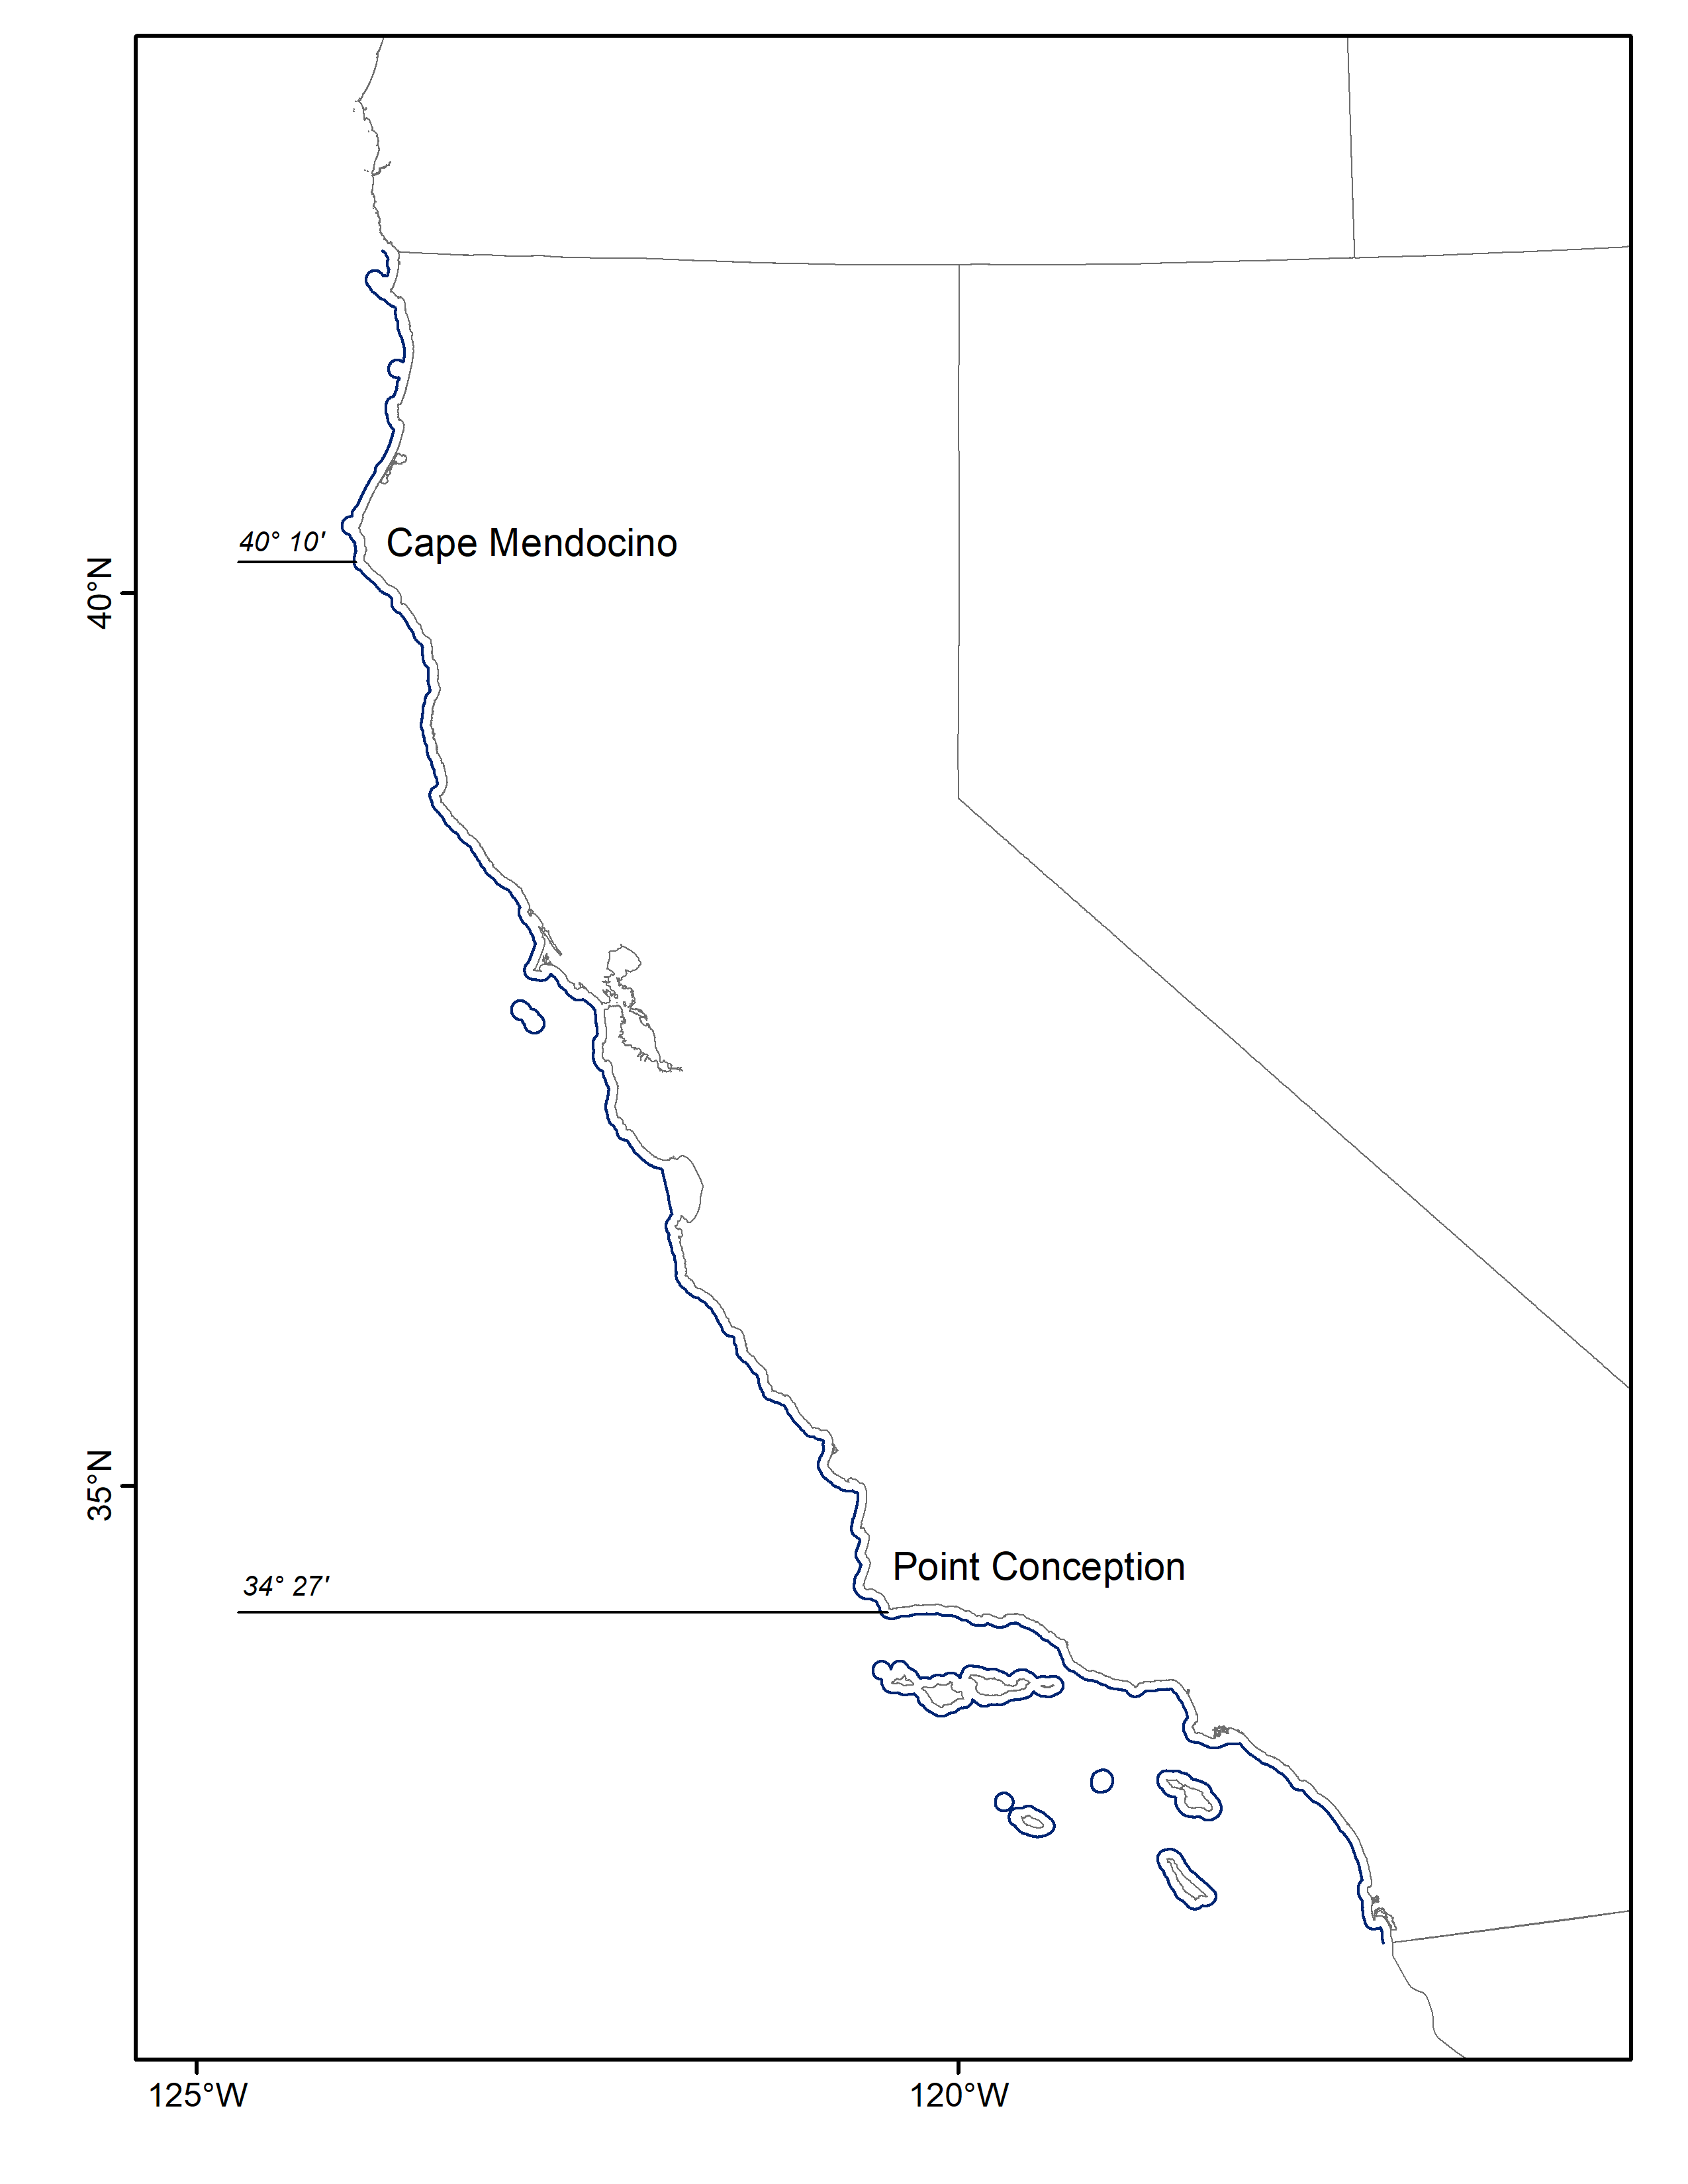
\includegraphics[width=1\textwidth,height=1\textheight]{C:/Stock_Assessments/VRML_Assessment_2021/GitHub/Vermilion_2021/doc/figures/assess_area.png}
\caption{Map of the assssment area with the 3 nm California stat water boundary. The northern California model includes areas from Pt. Conception to the California-Oregon border and the southern California assessment includes areas from Pt. Concpetion to the USA-Mexico border.\label{fig:assess-area}}
\end{figure}

\begin{figure}
\centering
\includegraphics[width=1\textwidth,height=1\textheight]{C:/Stock_Assessments/VRML_Assessment_2021/Model_files/NCA/Verm21NoCA_066_no_Don_P_rec_comps/plots/catch2 landings stacked.png}
\caption{Catches by fleet used in the base model.\label{fig:catch}}
\end{figure}

\begin{figure}
\centering
\includegraphics[width=0.5\textwidth,height=0.5\textheight]{C:/Stock_Assessments/VRML_Assessment_2021/Model_files/NCA/Verm21NoCA_066_no_Don_P_rec_comps/plots/comp_lendat_bubflt11mkt0.png}
\caption{Length composition data from the commercial hook-and-line fishery.\label{fig:len-data-COM-HKL}}
\end{figure}

\begin{figure}
\centering
\includegraphics[width=0.5\textwidth,height=0.5\textheight]{C:/Stock_Assessments/VRML_Assessment_2021/Model_files/NCA/Verm21NoCA_066_no_Don_P_rec_comps/plots/comp_lendat_data_weighting_TA1.8_COM_HKL.png}
\caption{Mean length for the commercial hook-and-line fishery with 95 percent confidence intervals.\label{fig:mean-com-len-data-COM-HKL}}
\end{figure}

\begin{figure}
\centering
\includegraphics[width=0.5\textwidth,height=0.5\textheight]{C:/Stock_Assessments/VRML_Assessment_2021/Model_files/NCA/Verm21NoCA_066_no_Don_P_rec_comps/plots/comp_lendat_bubflt2mkt0.png}
\caption{Length composition data from the commercial trawl fishery.\label{fig:len-data-COM-TWL}}
\end{figure}

\begin{figure}
\centering
\includegraphics[width=0.5\textwidth,height=0.5\textheight]{C:/Stock_Assessments/VRML_Assessment_2021/Model_files/NCA/Verm21NoCA_066_no_Don_P_rec_comps/plots/comp_lendat_data_weighting_TA1.8_COM_TWL.png}
\caption{Mean length for the commercial trawl fishery with 95 percent confidence intervals.\label{fig:mean-com-len-data-COM-TWL}}
\end{figure}

\begin{figure}
\centering
\includegraphics[width=0.5\textwidth,height=0.5\textheight]{C:/Stock_Assessments/VRML_Assessment_2021/Model_files/NCA/Verm21NoCA_066_no_Don_P_rec_comps/plots/comp_lendat_bubflt3mkt0.png}
\caption{Length composition data from the commercial net fishery.\label{fig:len-data-COM-NET}}
\end{figure}

\begin{figure}
\centering
\includegraphics[width=0.5\textwidth,height=0.5\textheight]{C:/Stock_Assessments/VRML_Assessment_2021/Model_files/NCA/Verm21NoCA_066_no_Don_P_rec_comps/plots/comp_lendat_data_weighting_TA1.8_COM_NET.png}
\caption{Mean length for the commercial net fishery with 95 percent confidence intervals.\label{fig:mean-com-len-data-COM-NET}}
\end{figure}

\begin{figure}
\centering
\includegraphics[width=0.5\textwidth,height=0.5\textheight]{C:/Stock_Assessments/VRML_Assessment_2021/Model_files/NCA/Verm21NoCA_066_no_Don_P_rec_comps/plots/comp_lendat_bubflt4mkt0_page2.png}
\caption{Length composition data from the recreational PC retained fishery.\label{fig:len-data-REC-PC}}
\end{figure}

\begin{figure}
\centering
\includegraphics[width=0.5\textwidth,height=0.5\textheight]{C:/Stock_Assessments/VRML_Assessment_2021/Model_files/NCA/Verm21NoCA_066_no_Don_P_rec_comps/plots/comp_lendat_data_weighting_TA1.8_REC_PC.png}
\caption{Mean length for the recreational PC retained fishery with 95 percent confidence intervals.\label{fig:mean-com-len-data-REC-PC}}
\end{figure}

\begin{figure}
\centering
\includegraphics[width=0.5\textwidth,height=0.5\textheight]{C:/Stock_Assessments/VRML_Assessment_2021/Model_files/NCA/Verm21NoCA_066_no_Don_P_rec_comps/plots/comp_lendat_bubflt5mkt0.png}
\caption{Length composition data from the recreational PC discard fishery.\label{fig:len-data-REC-PC-DIS}}
\end{figure}

\begin{figure}
\centering
\includegraphics[width=0.5\textwidth,height=0.5\textheight]{C:/Stock_Assessments/VRML_Assessment_2021/Model_files/NCA/Verm21NoCA_066_no_Don_P_rec_comps/plots/comp_lendat_data_weighting_TA1.8_REC_PC_DIS.png}
\caption{Mean length for the recreational PC discard fishery with 95 percent confidence intervals.\label{fig:mean-com-len-data-REC-PC-DIS}}
\end{figure}

\begin{figure}
\centering
\includegraphics[width=0.5\textwidth,height=0.5\textheight]{C:/Stock_Assessments/VRML_Assessment_2021/Model_files/NCA/Verm21NoCA_066_no_Don_P_rec_comps/plots/comp_lendat_bubflt6mkt0_page2.png}
\caption{Length composition data from the recreational PR retained fishery.\label{fig:len-data-REC-PR}}
\end{figure}

\begin{figure}
\centering
\includegraphics[width=0.5\textwidth,height=0.5\textheight]{C:/Stock_Assessments/VRML_Assessment_2021/Model_files/NCA/Verm21NoCA_066_no_Don_P_rec_comps/plots/comp_lendat_data_weighting_TA1.8_REC_PR.png}
\caption{Mean length for the recreational PR retained fishery with 95 percent confidence intervals.\label{fig:mean-com-len-data-REC-PR}}
\end{figure}

\begin{figure}
\centering
\includegraphics[width=0.5\textwidth,height=0.5\textheight]{C:/Stock_Assessments/VRML_Assessment_2021/Model_files/NCA/Verm21NoCA_066_no_Don_P_rec_comps/plots/comp_lendat_bubflt8mkt0.png}
\caption{Length composition data from the Deb Wilson-Vandenberg onboard survey.\label{fig:len-data-DWV-ONBOARD}}
\end{figure}

\begin{figure}
\centering
\includegraphics[width=0.5\textwidth,height=0.5\textheight]{C:/Stock_Assessments/VRML_Assessment_2021/Model_files/NCA/Verm21NoCA_066_no_Don_P_rec_comps/plots/comp_lendat_data_weighting_TA1.8_DWV_ONBOARD.png}
\caption{Mean length for the Deb Wilson-Vandenberg onboard survey with 95 percent confidence intervals.\label{fig:mean-com-len-data-DWV-ONBOARD}}
\end{figure}

\begin{figure}
\centering
\includegraphics[width=0.5\textwidth,height=0.5\textheight]{C:/Stock_Assessments/VRML_Assessment_2021/Model_files/NCA/Verm21NoCA_066_no_Don_P_rec_comps/plots/comp_lendat_bubflt9mkt0.png}
\caption{Length composition data from the West coast groundfish bottomfish trawl survey.\label{fig:len-data-NWFSC-TWL}}
\end{figure}

\begin{figure}
\centering
\includegraphics[width=0.5\textwidth,height=0.5\textheight]{C:/Stock_Assessments/VRML_Assessment_2021/Model_files/NCA/Verm21NoCA_066_no_Don_P_rec_comps/plots/comp_lendat_data_weighting_TA1.8_NWFSC_TWL.png}
\caption{Mean length for the West coast groundfish bottomfish trawl survey with 95 percent confidence intervals.\label{fig:mean-com-len-data-NWFSC-TWL}}
\end{figure}

\begin{figure}
\centering
\includegraphics[width=0.5\textwidth,height=0.5\textheight]{C:/Stock_Assessments/VRML_Assessment_2021/Model_files/NCA/Verm21NoCA_066_no_Don_P_rec_comps/plots/comp_lendat_bubflt11mkt0.png}
\caption{Length composition data from the Abrams thesis research survey.\label{fig:len-data-ABRAMS-RESEARCH}}
\end{figure}

\begin{figure}
\centering
\includegraphics[width=0.5\textwidth,height=0.5\textheight]{C:/Stock_Assessments/VRML_Assessment_2021/Model_files/NCA/Verm21NoCA_066_no_Don_P_rec_comps/plots/comp_lendat_data_weighting_TA1.8_ABRAMS_RESEARCH.png}
\caption{Mean length for the Abrams thesis research survey with 95 percent confidence intervals.\label{fig:mean-com-len-data-ABRAMS-RESEARCH}}
\end{figure}

\begin{figure}
\centering
\includegraphics[width=0.5\textwidth,height=0.5\textheight]{C:/Stock_Assessments/VRML_Assessment_2021/Model_files/NCA/Verm21NoCA_066_no_Don_P_rec_comps/plots/comp_lendat_bubflt12mkt0.png}
\caption{Length composition data from the SWFSC groundfish ecology survey.\label{fig:len-data-SWFSC-GF-ECOL}}
\end{figure}

\begin{figure}
\centering
\includegraphics[width=0.5\textwidth,height=0.5\textheight]{C:/Stock_Assessments/VRML_Assessment_2021/Model_files/NCA/Verm21NoCA_066_no_Don_P_rec_comps/plots/comp_lendat_data_weighting_TA1.8_SWFSC_GF_ECOL.png}
\caption{Mean length for the SWFSC groundfish ecology survey with 95 percent confidence intervals.\label{fig:mean-com-len-data-SWFSC-GF-ECOL}}
\end{figure}

\begin{figure}
\centering
\includegraphics[width=0.5\textwidth,height=0.5\textheight]{C:/Stock_Assessments/VRML_Assessment_2021/Model_files/NCA/Verm21NoCA_066_no_Don_P_rec_comps/plots/comp_lendat_bubflt13mkt0.png}
\caption{Length composition data from the California Collaborative Fisheries Research Project survey.\label{fig:len-data-CCFRP}}
\end{figure}

\begin{figure}
\centering
\includegraphics[width=0.5\textwidth,height=0.5\textheight]{C:/Stock_Assessments/VRML_Assessment_2021/Model_files/NCA/Verm21NoCA_066_no_Don_P_rec_comps/plots/comp_lendat_data_weighting_TA1.8_CCFRP.png}
\caption{Mean length for the California Collaborative Fisheries Research Project survey with 95 percent confidence intervals.\label{fig:mean-com-len-data-CCFRP}}
\end{figure}

\begin{figure}
\centering
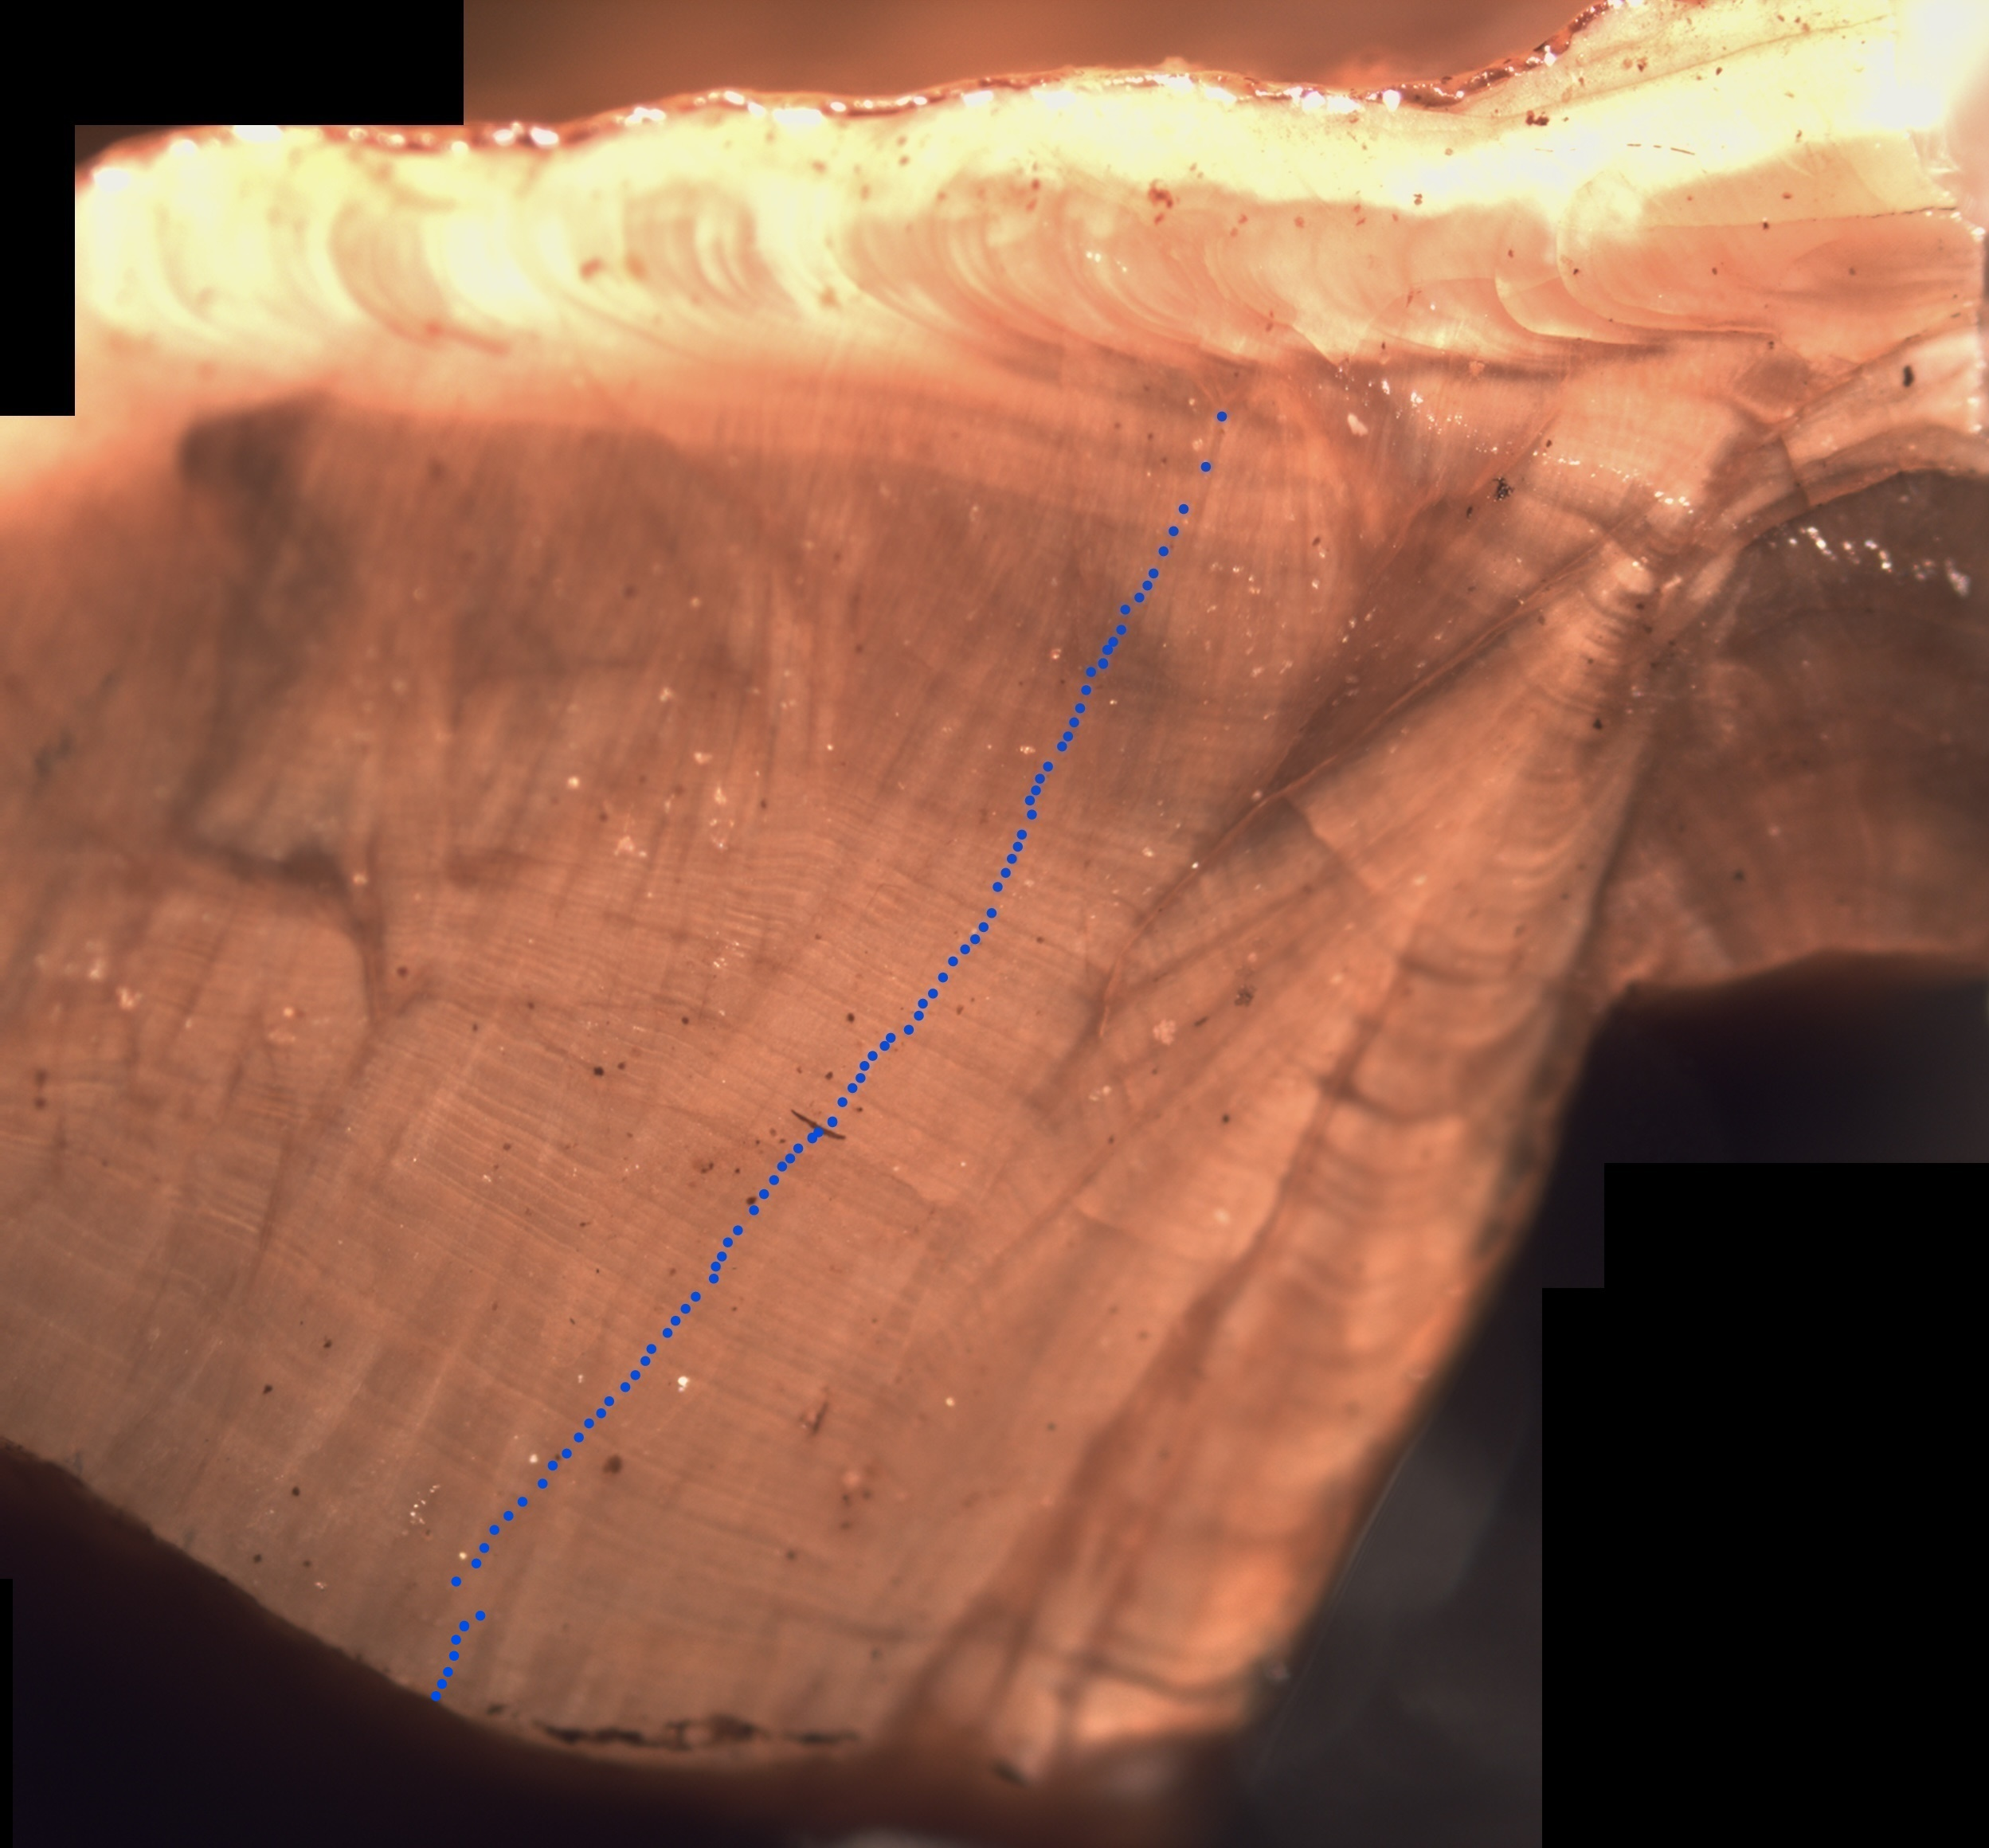
\includegraphics[width=1\textwidth,height=1\textheight]{C:/Stock_Assessments/VRML_Assessment_2021/GitHub/Vermilion_2021/doc/figures/oldfish.jpg}
\caption{Photograph of the \emph{oldest} aged fish used in the assessment with annuli marked by B. Kamikawa (NWFSC)..\label{fig:oldfish}}
\end{figure}

\begin{figure}
\centering
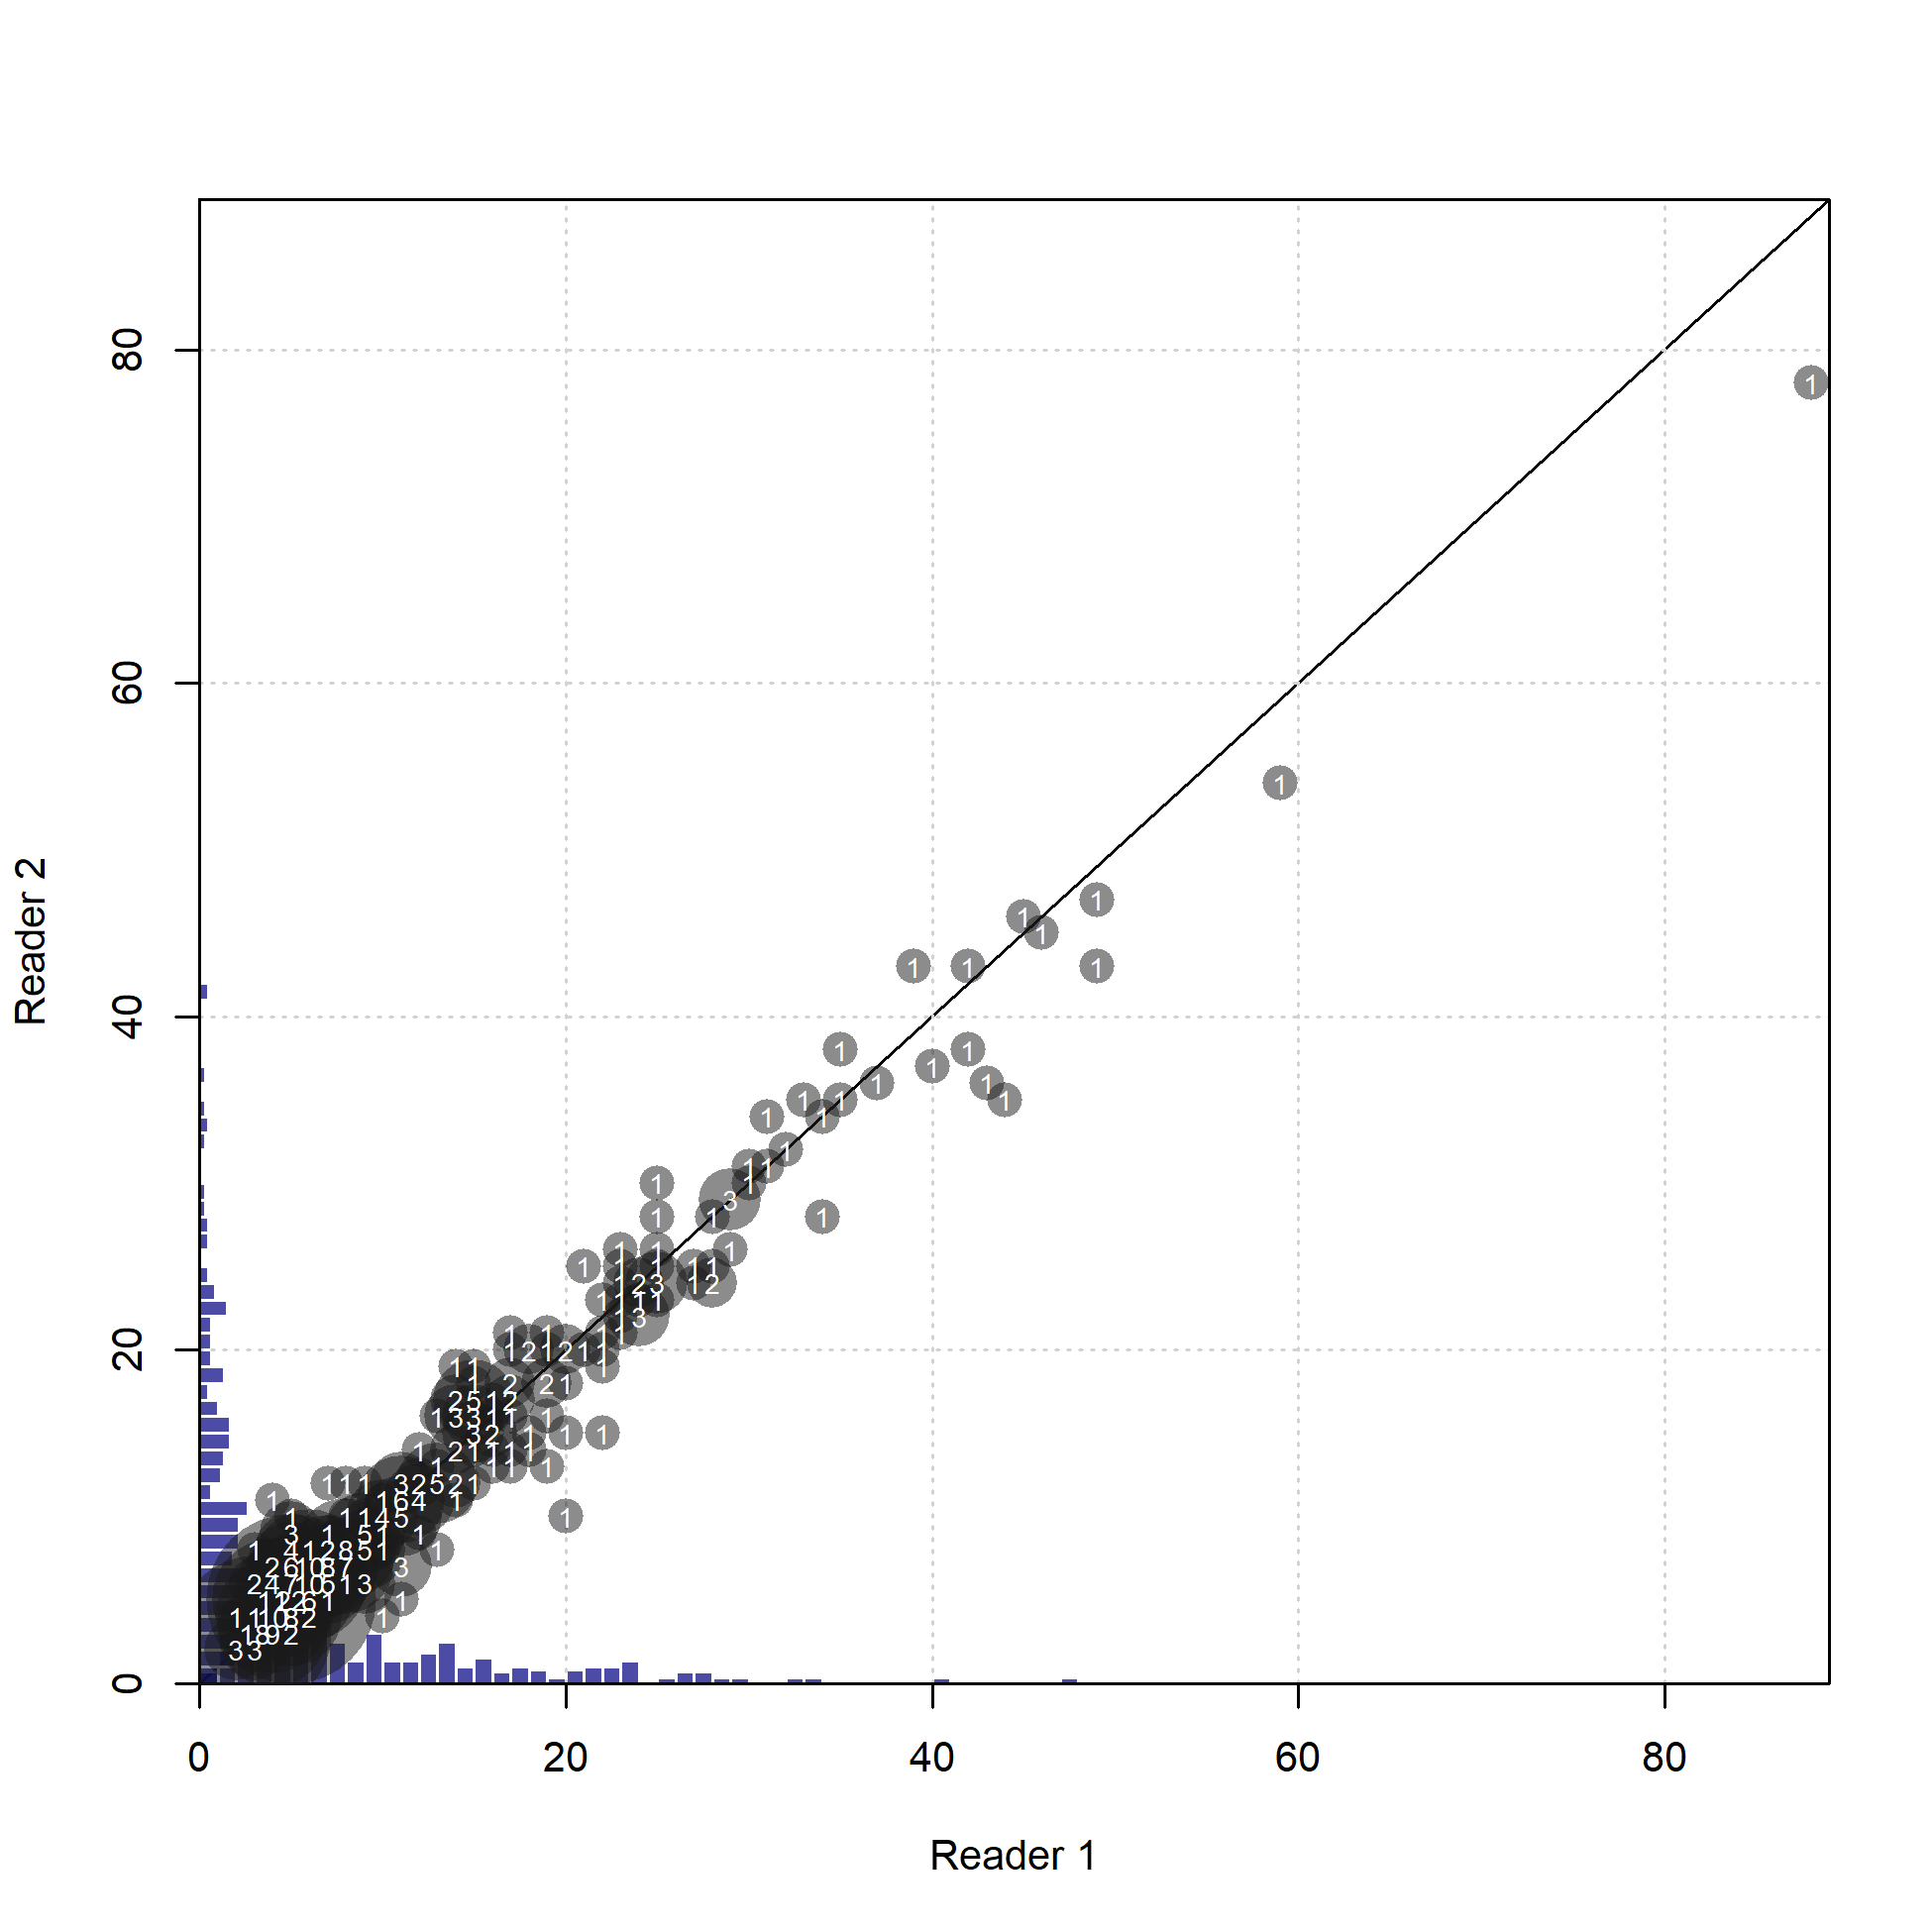
\includegraphics[width=1\textwidth,height=1\textheight]{C:/Stock_Assessments/VRML_Assessment_2021/GitHub/Vermilion_2021/doc/figures/Reader 1 vs Reader 2.png}
\caption{Aging precision between initial and blind double reads for vermilion. Numbers in the bubbles are the sample sizes of otoliths cross-read..\label{fig:reader1reader2}}
\end{figure}

\begin{figure}
\centering
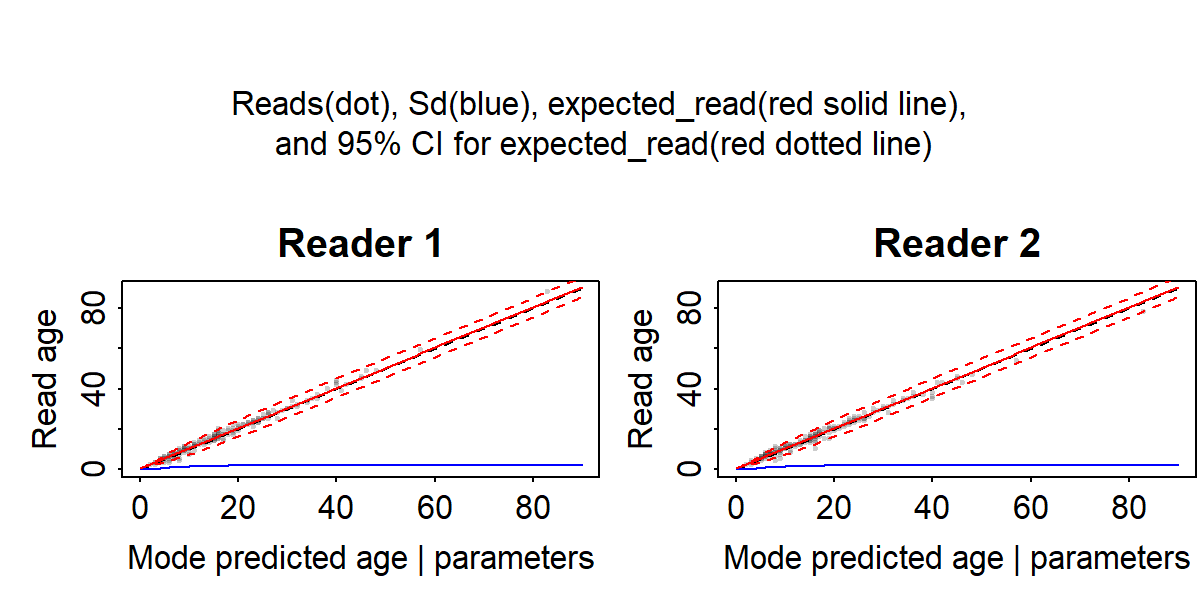
\includegraphics[width=1\textwidth,height=1\textheight]{C:/Stock_Assessments/VRML_Assessment_2021/GitHub/Vermilion_2021/doc/figures/True vs Reads (by reader).png}
\caption{True versus predicted age for two current age readers at the NWFSC from the ageing error software with unbiased reads for reader 1 and curvilinear bias for reader 1 and curvilinear standard deviation for both readers..\label{fig:truereads}}
\end{figure}

\begin{figure}
\centering
\includegraphics[width=1\textwidth,height=1\textheight]{C:/Stock_Assessments/VRML_Assessment_2021/Model_files/NCA/Verm21NoCA_066_no_Don_P_rec_comps/plots/numbers10_ageerror_matrix_1.png}
\caption{Distribution of observed age at true age for ageing error type 1.\label{fig:ageerror}}
\end{figure}

\begin{figure}
\centering
\includegraphics[width=1\textwidth,height=1\textheight]{C:/Stock_Assessments/VRML_Assessment_2021/Model_files/NCA/Verm21NoCA_066_no_Don_P_rec_comps/plots/bio1_sizeatage.png}
\caption{Length at age in the beginning of the year (or season) in the ending year of the model. Shaded area indicates 95\% distribution of length at age around estimated growth curve.\label{fig:fittedgrowth}}
\end{figure}

\begin{figure}
\centering
\includegraphics[width=1\textwidth,height=1\textheight]{C:/Stock_Assessments/VRML_Assessment_2021/Model_files/NCA/Verm21NoCA_066_no_Don_P_rec_comps/plots/bio5_weightatsize.png}
\caption{Weight-length relationship.\label{fig:weightlength}}
\end{figure}

\begin{figure}
\centering
\includegraphics[width=1\textwidth,height=1\textheight]{C:/Stock_Assessments/VRML_Assessment_2021/Model_files/NCA/Verm21NoCA_066_no_Don_P_rec_comps/plots/bio6_maturity.png}
\caption{Maturity at length.\label{fig:maturity}}
\end{figure}

\begin{figure}
\centering
\includegraphics[width=1\textwidth,height=1\textheight]{C:/Stock_Assessments/VRML_Assessment_2021/Model_files/NCA/Verm21NoCA_066_no_Don_P_rec_comps/plots/bio8_fecundity_wt.png}
\caption{Fecundity as a function of weight.\label{fig:fecundity}}
\end{figure}

\begin{figure}
\centering
\includegraphics[width=1\textwidth,height=1\textheight]{C:/Stock_Assessments/VRML_Assessment_2021/Model_files/NCA/Verm21NoCA_066_no_Don_P_rec_comps/plots/bio11_spawningoutput_age.png}
\caption{Spawning output at age. This is the product of maturity and fecundity. When these processes are length-based they are converted into the age dimension using the matrix of length at age.\label{fig:spawningoutputage}}
\end{figure}

\FloatBarrier

\FloatBarrier

\begin{figure}
\centering
\includegraphics[width=1\textwidth,height=1\textheight]{C:/Stock_Assessments/VRML_Assessment_2021/Model_files/NCA/Verm21NoCA_066_no_Don_P_rec_comps/plots/sel01_multiple_fleets_length1.png}
\caption{Selectivity at length by fleet.\label{fig:selex-length-all}}
\end{figure}

\FloatBarrier

\begin{figure}
\centering
\includegraphics[width=1\textwidth,height=1\textheight]{C:/Stock_Assessments/VRML_Assessment_2021/Model_files/NCA/Verm21NoCA_066_no_Don_P_rec_comps/plots/sel02_multiple_fleets_age1.png}
\caption{Selectivity at age derived from selectivity at length for multiple fleets.\label{fig:selex-age-all}}
\end{figure}

\begin{figure}
\centering
\includegraphics[width=1\textwidth,height=1\textheight]{C:/Stock_Assessments/VRML_Assessment_2021/Model_files/NCA/Verm21NoCA_066_no_Don_P_rec_comps/plots/sel03_len_timevary_surf_flt4sex1.png}
\caption{Surface plot of Female time-varying selectivity for REC\_PC.\label{fig:sel03_len_timevary_surf_flt4sex1}}
\end{figure}

\begin{figure}
\centering
\includegraphics[width=1\textwidth,height=1\textheight]{C:/Stock_Assessments/VRML_Assessment_2021/Model_files/NCA/Verm21NoCA_066_no_Don_P_rec_comps/plots/sel03_len_timevary_surf_flt6sex1.png}
\caption{Surface plot of Female time-varying selectivity for REC\_PR.\label{fig:sel03_len_timevary_surf_flt6sex1}}
\end{figure}

\begin{figure}
\centering
\includegraphics[width=1\textwidth,height=1\textheight]{C:/Stock_Assessments/VRML_Assessment_2021/Model_files/NCA/Verm21NoCA_066_no_Don_P_rec_comps/plots/sel03_len_timevary_surf_flt8sex1.png}
\caption{Surface plot of Female time-varying selectivity for DWV\_ONBOARD.\label{fig:sel03_len_timevary_surf_flt8sex1}}
\end{figure}

\begin{figure}
\centering
\includegraphics[width=1\textwidth,height=1\textheight]{C:/Stock_Assessments/VRML_Assessment_2021/Model_files/NCA/Verm21NoCA_066_no_Don_P_rec_comps/plots/sel03_len_timevary_surf_flt10sex1.png}
\caption{Surface plot of Female time-varying selectivity for REC\_PC\_ONBOARD.\label{fig:sel03_len_timevary_surf_flt10sex1}}
\end{figure}

\FloatBarrier

\FloatBarrier

\begin{figure}
\centering
\includegraphics[width=0.5\textwidth,height=0.5\textheight]{C:/Stock_Assessments/VRML_Assessment_2021/Model_files/NCA/Verm21NoCA_066_no_Don_P_rec_comps/plots/sel09_len_flt1sex1.png}
\caption{Female ending year selectivity for the commercial hook-and-line fishery.\label{fig:endyr-selex-COM-HKL}}
\end{figure}

\begin{figure}
\centering
\includegraphics[width=0.5\textwidth,height=0.5\textheight]{C:/Stock_Assessments/VRML_Assessment_2021/Model_files/NCA/Verm21NoCA_066_no_Don_P_rec_comps/plots/sel09_len_flt2sex1.png}
\caption{Female ending year selectivity for the commercial trawl fishery.\label{fig:endyr-selex-COM-TWL}}
\end{figure}

\begin{figure}
\centering
\includegraphics[width=0.5\textwidth,height=0.5\textheight]{C:/Stock_Assessments/VRML_Assessment_2021/Model_files/NCA/Verm21NoCA_066_no_Don_P_rec_comps/plots/sel09_len_flt3sex1.png}
\caption{Female ending year selectivity for the commercial net fishery.\label{fig:endyr-selex-COM-NET}}
\end{figure}

\begin{figure}
\centering
\includegraphics[width=0.5\textwidth,height=0.5\textheight]{C:/Stock_Assessments/VRML_Assessment_2021/Model_files/NCA/Verm21NoCA_066_no_Don_P_rec_comps/plots/sel09_len_flt4sex1.png}
\caption{Female ending year selectivity for the recreational PC retained fishery.\label{fig:endyr-selex-REC-PC}}
\end{figure}

\begin{figure}
\centering
\includegraphics[width=0.5\textwidth,height=0.5\textheight]{C:/Stock_Assessments/VRML_Assessment_2021/Model_files/NCA/Verm21NoCA_066_no_Don_P_rec_comps/plots/sel09_len_flt5sex1.png}
\caption{Female ending year selectivity for the recreational PC discard fishery.\label{fig:endyr-selex-REC-PC-DIS}}
\end{figure}

\begin{figure}
\centering
\includegraphics[width=0.5\textwidth,height=0.5\textheight]{C:/Stock_Assessments/VRML_Assessment_2021/Model_files/NCA/Verm21NoCA_066_no_Don_P_rec_comps/plots/sel09_len_flt6sex1.png}
\caption{Female ending year selectivity for the recreational PR retained fishery.\label{fig:endyr-selex-REC-PR}}
\end{figure}

\begin{figure}
\centering
\includegraphics[width=0.5\textwidth,height=0.5\textheight]{C:/Stock_Assessments/VRML_Assessment_2021/Model_files/NCA/Verm21NoCA_066_no_Don_P_rec_comps/plots/sel09_len_flt9sex1.png}
\caption{Female ending year selectivity for the West coast groundfish bottomfish trawl survey.\label{fig:endyr-selex-NWFSC-TWL}}
\end{figure}

\begin{figure}
\centering
\includegraphics[width=0.5\textwidth,height=0.5\textheight]{C:/Stock_Assessments/VRML_Assessment_2021/Model_files/NCA/Verm21NoCA_066_no_Don_P_rec_comps/plots/sel09_len_flt7sex1.png}
\caption{Female ending year selectivity for the recreational PR discard fishery.\label{fig:endyr-selex-REC-PR-DIS}}
\end{figure}

\FloatBarrier

\FloatBarrier

\begin{figure}
\centering
\includegraphics[width=1\textwidth,height=1\textheight]{C:/Stock_Assessments/VRML_Assessment_2021/Model_files/NCA/Verm21NoCA_066_no_Don_P_rec_comps/plots/comp_lenfit__aggregated_across_time.png}
\caption{Length comps, aggregated across time by fleet. Labels `retained' and `discard' indicate discarded or retained sampled for each fleet. Panels without this designation represent the whole catch.\label{fig:lenfits-all}}
\end{figure}

\begin{figure}
\centering
\includegraphics[width=0.5\textwidth,height=0.5\textheight]{C:/Stock_Assessments/VRML_Assessment_2021/Model_files/NCA/Verm21NoCA_066_no_Don_P_rec_comps/plots/comp_lenfit_residsflt11mkt0.png}
\caption{Pearson residuals for the commercial hook-and-line fishery. Closed bubbles are positive residuals (observed \textgreater{} expected) and open bubbles are negative residuals (observed \textless{} expected).\label{fig:len-pearson-COM-HKL}}
\end{figure}

\begin{figure}
\centering
\includegraphics[width=0.5\textwidth,height=0.5\textheight]{C:/Stock_Assessments/VRML_Assessment_2021/Model_files/NCA/Verm21NoCA_066_no_Don_P_rec_comps/plots/comp_lenfit_data_weighting_TA1.8_COM_HKL.png}
\caption{Mean length for REC\_PR with 95\% confidence intervals based on current samples sizes. Francis data weighting method TA1.8: thinner intervals (with capped ends) show result of further adjusting sample sizes based on suggested multiplier (with 95\% interval) for length data from the commercial hook-and-line fishery.\label{fig:mean-len-fit-COM-HKL}}
\end{figure}

\begin{figure}
\centering
\includegraphics[width=0.5\textwidth,height=0.5\textheight]{C:/Stock_Assessments/VRML_Assessment_2021/Model_files/NCA/Verm21NoCA_066_no_Don_P_rec_comps/plots/comp_lenfit_residsflt2mkt0.png}
\caption{Pearson residuals for the commercial trawl fishery. Closed bubbles are positive residuals (observed \textgreater{} expected) and open bubbles are negative residuals (observed \textless{} expected).\label{fig:len-pearson-COM-TWL}}
\end{figure}

\begin{figure}
\centering
\includegraphics[width=0.5\textwidth,height=0.5\textheight]{C:/Stock_Assessments/VRML_Assessment_2021/Model_files/NCA/Verm21NoCA_066_no_Don_P_rec_comps/plots/comp_lenfit_data_weighting_TA1.8_COM_TWL.png}
\caption{Mean length for REC\_PR with 95\% confidence intervals based on current samples sizes. Francis data weighting method TA1.8: thinner intervals (with capped ends) show result of further adjusting sample sizes based on suggested multiplier (with 95\% interval) for length data from the commercial trawl fishery.\label{fig:mean-len-fit-COM-TWL}}
\end{figure}

\begin{figure}
\centering
\includegraphics[width=0.5\textwidth,height=0.5\textheight]{C:/Stock_Assessments/VRML_Assessment_2021/Model_files/NCA/Verm21NoCA_066_no_Don_P_rec_comps/plots/comp_lenfit_residsflt3mkt0.png}
\caption{Pearson residuals for the commercial net fishery. Closed bubbles are positive residuals (observed \textgreater{} expected) and open bubbles are negative residuals (observed \textless{} expected).\label{fig:len-pearson-COM-NET}}
\end{figure}

\begin{figure}
\centering
\includegraphics[width=0.5\textwidth,height=0.5\textheight]{C:/Stock_Assessments/VRML_Assessment_2021/Model_files/NCA/Verm21NoCA_066_no_Don_P_rec_comps/plots/comp_lenfit_data_weighting_TA1.8_COM_NET.png}
\caption{Mean length for REC\_PR with 95\% confidence intervals based on current samples sizes. Francis data weighting method TA1.8: thinner intervals (with capped ends) show result of further adjusting sample sizes based on suggested multiplier (with 95\% interval) for length data from the commercial net fishery.\label{fig:mean-len-fit-COM-NET}}
\end{figure}

\begin{figure}
\centering
\includegraphics[width=0.5\textwidth,height=0.5\textheight]{C:/Stock_Assessments/VRML_Assessment_2021/Model_files/NCA/Verm21NoCA_066_no_Don_P_rec_comps/plots/comp_lenfit_residsflt4mkt0_page2.png}
\caption{Pearson residuals for the recreational PC retained fishery. Closed bubbles are positive residuals (observed \textgreater{} expected) and open bubbles are negative residuals (observed \textless{} expected).\label{fig:len-pearson-REC-PC}}
\end{figure}

\begin{figure}
\centering
\includegraphics[width=0.5\textwidth,height=0.5\textheight]{C:/Stock_Assessments/VRML_Assessment_2021/Model_files/NCA/Verm21NoCA_066_no_Don_P_rec_comps/plots/comp_lenfit_data_weighting_TA1.8_REC_PC.png}
\caption{Mean length for REC\_PR with 95\% confidence intervals based on current samples sizes. Francis data weighting method TA1.8: thinner intervals (with capped ends) show result of further adjusting sample sizes based on suggested multiplier (with 95\% interval) for length data from the recreational PC retained fishery.\label{fig:mean-len-fit-REC-PC}}
\end{figure}

\begin{figure}
\centering
\includegraphics[width=0.5\textwidth,height=0.5\textheight]{C:/Stock_Assessments/VRML_Assessment_2021/Model_files/NCA/Verm21NoCA_066_no_Don_P_rec_comps/plots/comp_lenfit_residsflt5mkt0.png}
\caption{Pearson residuals for the recreational PC discard fishery. Closed bubbles are positive residuals (observed \textgreater{} expected) and open bubbles are negative residuals (observed \textless{} expected).\label{fig:len-pearson-REC-PC-DIS}}
\end{figure}

\begin{figure}
\centering
\includegraphics[width=0.5\textwidth,height=0.5\textheight]{C:/Stock_Assessments/VRML_Assessment_2021/Model_files/NCA/Verm21NoCA_066_no_Don_P_rec_comps/plots/comp_lenfit_data_weighting_TA1.8_REC_PC_DIS.png}
\caption{Mean length for REC\_PR with 95\% confidence intervals based on current samples sizes. Francis data weighting method TA1.8: thinner intervals (with capped ends) show result of further adjusting sample sizes based on suggested multiplier (with 95\% interval) for length data from the recreational PC discard fishery.\label{fig:mean-len-fit-REC-PC-DIS}}
\end{figure}

\begin{figure}
\centering
\includegraphics[width=0.5\textwidth,height=0.5\textheight]{C:/Stock_Assessments/VRML_Assessment_2021/Model_files/NCA/Verm21NoCA_066_no_Don_P_rec_comps/plots/comp_lenfit_residsflt6mkt0_page2.png}
\caption{Pearson residuals for the recreational PR retained fishery. Closed bubbles are positive residuals (observed \textgreater{} expected) and open bubbles are negative residuals (observed \textless{} expected).\label{fig:len-pearson-REC-PR}}
\end{figure}

\begin{figure}
\centering
\includegraphics[width=0.5\textwidth,height=0.5\textheight]{C:/Stock_Assessments/VRML_Assessment_2021/Model_files/NCA/Verm21NoCA_066_no_Don_P_rec_comps/plots/comp_lenfit_data_weighting_TA1.8_REC_PR.png}
\caption{Mean length for REC\_PR with 95\% confidence intervals based on current samples sizes. Francis data weighting method TA1.8: thinner intervals (with capped ends) show result of further adjusting sample sizes based on suggested multiplier (with 95\% interval) for length data from the recreational PR retained fishery.\label{fig:mean-len-fit-REC-PR}}
\end{figure}

\begin{figure}
\centering
\includegraphics[width=0.5\textwidth,height=0.5\textheight]{C:/Stock_Assessments/VRML_Assessment_2021/Model_files/NCA/Verm21NoCA_066_no_Don_P_rec_comps/plots/comp_lenfit_residsflt8mkt0.png}
\caption{Pearson residuals for the Deb Wilson-Vandenberg onboard survey. Closed bubbles are positive residuals (observed \textgreater{} expected) and open bubbles are negative residuals (observed \textless{} expected).\label{fig:len-pearson-DWV-ONBOARD}}
\end{figure}

\begin{figure}
\centering
\includegraphics[width=0.5\textwidth,height=0.5\textheight]{C:/Stock_Assessments/VRML_Assessment_2021/Model_files/NCA/Verm21NoCA_066_no_Don_P_rec_comps/plots/comp_lenfit_data_weighting_TA1.8_DWV_ONBOARD.png}
\caption{Mean length for REC\_PR with 95\% confidence intervals based on current samples sizes. Francis data weighting method TA1.8: thinner intervals (with capped ends) show result of further adjusting sample sizes based on suggested multiplier (with 95\% interval) for length data from the Deb Wilson-Vandenberg onboard survey.\label{fig:mean-len-fit-DWV-ONBOARD}}
\end{figure}

\begin{figure}
\centering
\includegraphics[width=0.5\textwidth,height=0.5\textheight]{C:/Stock_Assessments/VRML_Assessment_2021/Model_files/NCA/Verm21NoCA_066_no_Don_P_rec_comps/plots/comp_lenfit_residsflt9mkt0.png}
\caption{Pearson residuals for the West coast groundfish bottomfish trawl survey. Closed bubbles are positive residuals (observed \textgreater{} expected) and open bubbles are negative residuals (observed \textless{} expected).\label{fig:len-pearson-NWFSC-TWL}}
\end{figure}

\begin{figure}
\centering
\includegraphics[width=0.5\textwidth,height=0.5\textheight]{C:/Stock_Assessments/VRML_Assessment_2021/Model_files/NCA/Verm21NoCA_066_no_Don_P_rec_comps/plots/comp_lenfit_data_weighting_TA1.8_NWFSC_TWL.png}
\caption{Mean length for REC\_PR with 95\% confidence intervals based on current samples sizes. Francis data weighting method TA1.8: thinner intervals (with capped ends) show result of further adjusting sample sizes based on suggested multiplier (with 95\% interval) for length data from the West coast groundfish bottomfish trawl survey.\label{fig:mean-len-fit-NWFSC-TWL}}
\end{figure}

\begin{figure}
\centering
\includegraphics[width=0.5\textwidth,height=0.5\textheight]{C:/Stock_Assessments/VRML_Assessment_2021/Model_files/NCA/Verm21NoCA_066_no_Don_P_rec_comps/plots/comp_lenfit_residsflt11mkt0.png}
\caption{Pearson residuals for the Abrams thesis research survey. Closed bubbles are positive residuals (observed \textgreater{} expected) and open bubbles are negative residuals (observed \textless{} expected).\label{fig:len-pearson-ABRAMS-RESEARCH}}
\end{figure}

\begin{figure}
\centering
\includegraphics[width=0.5\textwidth,height=0.5\textheight]{C:/Stock_Assessments/VRML_Assessment_2021/Model_files/NCA/Verm21NoCA_066_no_Don_P_rec_comps/plots/comp_lenfit_data_weighting_TA1.8_ABRAMS_RESEARCH.png}
\caption{Mean length for REC\_PR with 95\% confidence intervals based on current samples sizes. Francis data weighting method TA1.8: thinner intervals (with capped ends) show result of further adjusting sample sizes based on suggested multiplier (with 95\% interval) for length data from the Abrams thesis research survey.\label{fig:mean-len-fit-ABRAMS-RESEARCH}}
\end{figure}

\begin{figure}
\centering
\includegraphics[width=0.5\textwidth,height=0.5\textheight]{C:/Stock_Assessments/VRML_Assessment_2021/Model_files/NCA/Verm21NoCA_066_no_Don_P_rec_comps/plots/comp_lenfit_residsflt12mkt0.png}
\caption{Pearson residuals for the SWFSC groundfish ecology survey. Closed bubbles are positive residuals (observed \textgreater{} expected) and open bubbles are negative residuals (observed \textless{} expected).\label{fig:len-pearson-SWFSC-GF-ECOL}}
\end{figure}

\begin{figure}
\centering
\includegraphics[width=0.5\textwidth,height=0.5\textheight]{C:/Stock_Assessments/VRML_Assessment_2021/Model_files/NCA/Verm21NoCA_066_no_Don_P_rec_comps/plots/comp_lenfit_data_weighting_TA1.8_SWFSC_GF_ECOL.png}
\caption{Mean length for REC\_PR with 95\% confidence intervals based on current samples sizes. Francis data weighting method TA1.8: thinner intervals (with capped ends) show result of further adjusting sample sizes based on suggested multiplier (with 95\% interval) for length data from the SWFSC groundfish ecology survey.\label{fig:mean-len-fit-SWFSC-GF-ECOL}}
\end{figure}

\begin{figure}
\centering
\includegraphics[width=0.5\textwidth,height=0.5\textheight]{C:/Stock_Assessments/VRML_Assessment_2021/Model_files/NCA/Verm21NoCA_066_no_Don_P_rec_comps/plots/comp_lenfit_residsflt13mkt0.png}
\caption{Pearson residuals for the California Collaborative Fisheries Research Project survey. Closed bubbles are positive residuals (observed \textgreater{} expected) and open bubbles are negative residuals (observed \textless{} expected).\label{fig:len-pearson-CCFRP}}
\end{figure}

\begin{figure}
\centering
\includegraphics[width=0.5\textwidth,height=0.5\textheight]{C:/Stock_Assessments/VRML_Assessment_2021/Model_files/NCA/Verm21NoCA_066_no_Don_P_rec_comps/plots/comp_lenfit_data_weighting_TA1.8_CCFRP.png}
\caption{Mean length for REC\_PR with 95\% confidence intervals based on current samples sizes. Francis data weighting method TA1.8: thinner intervals (with capped ends) show result of further adjusting sample sizes based on suggested multiplier (with 95\% interval) for length data from the California Collaborative Fisheries Research Project survey.\label{fig:mean-len-fit-CCFRP}}
\end{figure}

\begin{figure}
\centering
\includegraphics[width=0.5\textwidth,height=0.5\textheight]{C:/Stock_Assessments/VRML_Assessment_2021/Model_files/NCA/Verm21NoCA_066_no_Don_P_rec_comps/plots/sexratio_len_flt11mkt0.png}
\caption{Sex ratios for length comps, whole catchAbrams thesis research survey. Observed sex ratios (points) with 75\% intervals (vertical lines) calculated as a Jeffreys interval based on the adjusted input sample size. The model expectation is shown in the purple line.\label{fig:sexratio-ABRAMS-RESEARCH}}
\end{figure}

\begin{figure}
\centering
\includegraphics[width=0.5\textwidth,height=0.5\textheight]{C:/Stock_Assessments/VRML_Assessment_2021/Model_files/NCA/Verm21NoCA_066_no_Don_P_rec_comps/plots/sexratio_len_flt12mkt0.png}
\caption{Sex ratios for length comps, whole catchSWFSC groundfish ecology survey. Observed sex ratios (points) with 75\% intervals (vertical lines) calculated as a Jeffreys interval based on the adjusted input sample size. The model expectation is shown in the purple line.\label{fig:sexratio-SWFSC-GF-ECOL}}
\end{figure}

\begin{figure}
\centering
\includegraphics[width=0.5\textwidth,height=0.5\textheight]{C:/Stock_Assessments/VRML_Assessment_2021/Model_files/NCA/Verm21NoCA_066_no_Don_P_rec_comps/plots/sexratio_len_flt9mkt0.png}
\caption{Sex ratios for length comps, whole catchWest coast groundfish bottomfish trawl survey. Observed sex ratios (points) with 75\% intervals (vertical lines) calculated as a Jeffreys interval based on the adjusted input sample size. The model expectation is shown in the purple line.\label{fig:sexratio-NWFSC-TWL}}
\end{figure}

\FloatBarrier

\begin{figure}
\centering
\includegraphics[width=1\textwidth,height=1\textheight]{C:/Stock_Assessments/VRML_Assessment_2021/Model_files/NCA/Verm21NoCA_066_no_Don_P_rec_comps/plots/ts7_Spawning_output_with_95_asymptotic_intervals_intervals.png}
\caption{Estimated time series of spawning output.\label{fig:ssb}}
\end{figure}

\begin{figure}
\centering
\includegraphics[width=1\textwidth,height=1\textheight]{C:/Stock_Assessments/VRML_Assessment_2021/Model_files/NCA/Verm21NoCA_066_no_Don_P_rec_comps/plots/ts9_Relative_spawning_output_intervals.png}
\caption{Estimated time series of relative spawning output.\label{fig:depl}}
\end{figure}

\FloatBarrier

\begin{figure}
\centering
\includegraphics[width=0.5\textwidth,height=0.5\textheight]{C:/Stock_Assessments/VRML_Assessment_2021/Model_files/NCA/Verm21NoCA_066_no_Don_P_rec_comps/plots/index9_standcpueall.png}
\caption{Standardized indices overlaid. Each index is rescaled to have mean observation = 1.0.\label{fig:cpueall}}
\end{figure}

\begin{figure}
\centering
\includegraphics[width=0.5\textwidth,height=0.5\textheight]{C:/Stock_Assessments/VRML_Assessment_2021/Model_files/NCA/Verm21NoCA_066_no_Don_P_rec_comps/plots/index5_logcpuefit_REC_PC.png}
\caption{Fit to log index data on log scale for the recreational PC retained fishery. Lines indicate 95\% uncertainty interval around index values based on the model assumption of lognormal error. Thicker lines (if present) indicate input uncertainty before addition of estimated additional uncertainty parameter.\label{fig:log-cpue-REC-PC}}
\end{figure}

\begin{figure}
\centering
\includegraphics[width=0.5\textwidth,height=0.5\textheight]{C:/Stock_Assessments/VRML_Assessment_2021/Model_files/NCA/Verm21NoCA_066_no_Don_P_rec_comps/plots/index10_resids_SE_total_REC_PC.png}
\caption{Residuals of fit to index for the REC\_PC. Values are (log(Obs) - log(Exp))/SE where SE is the total standard error including any estimated additional uncertainty.\label{fig:cpue-resid-REC-PC}}
\end{figure}

\begin{figure}
\centering
\includegraphics[width=0.5\textwidth,height=0.5\textheight]{C:/Stock_Assessments/VRML_Assessment_2021/Model_files/NCA/Verm21NoCA_066_no_Don_P_rec_comps/plots/index5_logcpuefit_REC_PR.png}
\caption{Fit to log index data on log scale for the recreational PR retained fishery. Lines indicate 95\% uncertainty interval around index values based on the model assumption of lognormal error. Thicker lines (if present) indicate input uncertainty before addition of estimated additional uncertainty parameter.\label{fig:log-cpue-REC-PR}}
\end{figure}

\begin{figure}
\centering
\includegraphics[width=0.5\textwidth,height=0.5\textheight]{C:/Stock_Assessments/VRML_Assessment_2021/Model_files/NCA/Verm21NoCA_066_no_Don_P_rec_comps/plots/index10_resids_SE_total_REC_PR.png}
\caption{Residuals of fit to index for the REC\_PR. Values are (log(Obs) - log(Exp))/SE where SE is the total standard error including any estimated additional uncertainty.\label{fig:cpue-resid-REC-PR}}
\end{figure}

\begin{figure}
\centering
\includegraphics[width=0.5\textwidth,height=0.5\textheight]{C:/Stock_Assessments/VRML_Assessment_2021/Model_files/NCA/Verm21NoCA_066_no_Don_P_rec_comps/plots/index5_logcpuefit_DWV_ONBOARD.png}
\caption{Fit to log index data on log scale for the Deb Wilson-Vandenberg onboard survey. Lines indicate 95\% uncertainty interval around index values based on the model assumption of lognormal error. Thicker lines (if present) indicate input uncertainty before addition of estimated additional uncertainty parameter.\label{fig:log-cpue-DWV-ONBOARD}}
\end{figure}

\begin{figure}
\centering
\includegraphics[width=0.5\textwidth,height=0.5\textheight]{C:/Stock_Assessments/VRML_Assessment_2021/Model_files/NCA/Verm21NoCA_066_no_Don_P_rec_comps/plots/index10_resids_SE_total_DWV_ONBOARD.png}
\caption{Residuals of fit to index for the DWV\_ONBOARD. Values are (log(Obs) - log(Exp))/SE where SE is the total standard error including any estimated additional uncertainty.\label{fig:cpue-resid-DWV-ONBOARD}}
\end{figure}

\begin{figure}
\centering
\includegraphics[width=0.5\textwidth,height=0.5\textheight]{C:/Stock_Assessments/VRML_Assessment_2021/Model_files/NCA/Verm21NoCA_066_no_Don_P_rec_comps/plots/index5_logcpuefit_NWFSC_TWL.png}
\caption{Fit to log index data on log scale for the West coast groundfish bottomfish trawl survey. Lines indicate 95\% uncertainty interval around index values based on the model assumption of lognormal error. Thicker lines (if present) indicate input uncertainty before addition of estimated additional uncertainty parameter.\label{fig:log-cpue-NWFSC-TWL}}
\end{figure}

\begin{figure}
\centering
\includegraphics[width=0.5\textwidth,height=0.5\textheight]{C:/Stock_Assessments/VRML_Assessment_2021/Model_files/NCA/Verm21NoCA_066_no_Don_P_rec_comps/plots/index10_resids_SE_total_NWFSC_TWL.png}
\caption{Residuals of fit to index for the NWFSC\_TWL. Values are (log(Obs) - log(Exp))/SE where SE is the total standard error including any estimated additional uncertainty.\label{fig:cpue-resid-NWFSC-TWL}}
\end{figure}

\begin{figure}
\centering
\includegraphics[width=0.5\textwidth,height=0.5\textheight]{C:/Stock_Assessments/VRML_Assessment_2021/Model_files/NCA/Verm21NoCA_066_no_Don_P_rec_comps/plots/index5_logcpuefit_REC_PC_ONBOARD.png}
\caption{Fit to log index data on log scale for the recreational PC onboard survey. Lines indicate 95\% uncertainty interval around index values based on the model assumption of lognormal error. Thicker lines (if present) indicate input uncertainty before addition of estimated additional uncertainty parameter.\label{fig:log-cpue-REC-PC-ONBOARD}}
\end{figure}

\begin{figure}
\centering
\includegraphics[width=0.5\textwidth,height=0.5\textheight]{C:/Stock_Assessments/VRML_Assessment_2021/Model_files/NCA/Verm21NoCA_066_no_Don_P_rec_comps/plots/index10_resids_SE_total_REC_PC_ONBOARD.png}
\caption{Residuals of fit to index for the REC\_PC\_ONBOARD. Values are (log(Obs) - log(Exp))/SE where SE is the total standard error including any estimated additional uncertainty.\label{fig:cpue-resid-REC-PC-ONBOARD}}
\end{figure}

\begin{figure}
\centering
\includegraphics[width=0.5\textwidth,height=0.5\textheight]{C:/Stock_Assessments/VRML_Assessment_2021/Model_files/NCA/Verm21NoCA_066_no_Don_P_rec_comps/plots/index5_logcpuefit_CCFRP.png}
\caption{Fit to log index data on log scale for the California Collaborative Fisheries Research Project survey. Lines indicate 95\% uncertainty interval around index values based on the model assumption of lognormal error. Thicker lines (if present) indicate input uncertainty before addition of estimated additional uncertainty parameter.\label{fig:log-cpue-CCFRP}}
\end{figure}

\begin{figure}
\centering
\includegraphics[width=0.5\textwidth,height=0.5\textheight]{C:/Stock_Assessments/VRML_Assessment_2021/Model_files/NCA/Verm21NoCA_066_no_Don_P_rec_comps/plots/index10_resids_SE_total_CCFRP.png}
\caption{Residuals of fit to index for the CCFRP. Values are (log(Obs) - log(Exp))/SE where SE is the total standard error including any estimated additional uncertainty.\label{fig:cpue-resid-CCFRP}}
\end{figure}

\begin{figure}
\centering
\includegraphics[width=1\textwidth,height=1\textheight]{C:/Stock_Assessments/VRML_Assessment_2021/Model_files/NCA/Verm21NoCA_066_no_Don_P_rec_comps/plots/comp_condAALfit_residsflt9mkt0_page1.png}
\caption{Pearson residuals, whole catch, NWFSC\_TWL (max=46.84) (plot 1 of 3).\label{fig:comp_condAALfit_residsflt9mkt0_page1}}
\end{figure}

\begin{figure}
\centering
\includegraphics[width=1\textwidth,height=1\textheight]{C:/Stock_Assessments/VRML_Assessment_2021/Model_files/NCA/Verm21NoCA_066_no_Don_P_rec_comps/plots/comp_condAALfit_residsflt9mkt0_page2.png}
\caption{Pearson residuals, whole catch, NWFSC\_TWL (max=46.84) (plot 1 of 3) (plot 2 of 3).\label{fig:comp_condAALfit_residsflt9mkt0_page2}}
\end{figure}

\begin{figure}
\centering
\includegraphics[width=1\textwidth,height=1\textheight]{C:/Stock_Assessments/VRML_Assessment_2021/Model_files/NCA/Verm21NoCA_066_no_Don_P_rec_comps/plots/comp_condAALfit_residsflt9mkt0_page3.png}
\caption{Pearson residuals, whole catch, NWFSC\_TWL (max=46.84) (plot 1 of 3) (plot 2 of 3) (plot 3 of 3).\label{fig:comp_condAALfit_residsflt9mkt0_page3}}
\end{figure}

\begin{figure}
\centering
\includegraphics[width=1\textwidth,height=1\textheight]{C:/Stock_Assessments/VRML_Assessment_2021/Model_files/NCA/Verm21NoCA_066_no_Don_P_rec_comps/plots/comp_condAALfit_residsflt11mkt0.png}
\caption{Pearson residuals, whole catch, ABRAMS\_RESEARCH (max=10.34).\label{fig:comp_condAALfit_residsflt11mkt0}}
\end{figure}

\begin{figure}
\centering
\includegraphics[width=1\textwidth,height=1\textheight]{C:/Stock_Assessments/VRML_Assessment_2021/Model_files/NCA/Verm21NoCA_066_no_Don_P_rec_comps/plots/comp_condAALfit_residsflt12mkt0.png}
\caption{Pearson residuals, whole catch, SWFSC\_GF\_ECOL (max=42.2).\label{fig:comp_condAALfit_residsflt12mkt0}}
\end{figure}

!{[}Mean age from conditional data (aggregated across length bins) for NWFSC\_TWL with 95\% confidence intervals based on current samples sizes.Francis data weighting method TA1.8: thinner intervals (with capped ends) show result of further adjusting sample sizes based on suggested multiplier (with 95\% interval) for conditional age-at-length data from NWFSC\_TWL:0.9906 (0.5346-4.2938) For more info, see

Francis, R.I.C.C. (2011). Data weighting in statistical fisheries stock assessment models. Can. J. Fish. Aquat. Sci. 68: 1124-1138.

.\label{fig:comp_condAALfit_data_weighting_TA1.8_condAgeNWFSC_TWL}{]}(C:/Stock\_Assessments/VRML\_Assessment\_2021/Model\_files/NCA/Verm21NoCA\_066\_no\_Don\_P\_rec\_comps/plots/comp\_condAALfit\_data\_weighting\_TA1.8\_condAgeNWFSC\_TWL.png)\{width=100\% height=100\% alt="Mean age from conditional data (aggregated across length bins) for NWFSC\_TWL with 95\% confidence intervals based on current samples sizes.Francis data weighting method TA1.8: thinner intervals (with capped ends) show result of further adjusting sample sizes based on suggested multiplier (with 95\% interval) for conditional age-at-length data from NWFSC\_TWL:0.9906 (0.5346-4.2938) For more info, see

Francis, R.I.C.C. (2011). Data weighting in statistical fisheries stock assessment models. Can. J. Fish. Aquat. Sci. 68: 1124-1138.

."\}

\begin{figure}
\centering
\includegraphics[width=1\textwidth,height=1\textheight]{C:/Stock_Assessments/VRML_Assessment_2021/Model_files/NCA/Verm21NoCA_066_no_Don_P_rec_comps/plots/comp_condAALfit_Andre_plotsflt9mkt0_page1.png}
\caption{Conditional AAL plot, whole catch, NWFSC\_TWL (plot 1 of 4) These plots show mean age and std. dev. in conditional {\tagstructbegin{tag=Link}\tagmcbegin{tag=Link}\href{mailto:A@L}{\nolinkurl{A@L}}\leavevmode\tagmcend\tagstructend}.Left plots are mean {\tagstructbegin{tag=Link}\tagmcbegin{tag=Link}\href{mailto:A@L}{\nolinkurl{A@L}}\leavevmode\tagmcend\tagstructend} by size-class (obs. and exp.) with 90\% CIs based on adding 1.64 SE of mean to the data.Right plots in each pair are SE of mean {\tagstructbegin{tag=Link}\tagmcbegin{tag=Link}\href{mailto:A@L}{\nolinkurl{A@L}}\leavevmode\tagmcend\tagstructend} (obs. and exp.) with 90\% CIs based on the chi-square distribution..\label{fig:comp_condAALfit_Andre_plotsflt9mkt0_page1}}
\end{figure}

\begin{figure}
\centering
\includegraphics[width=1\textwidth,height=1\textheight]{C:/Stock_Assessments/VRML_Assessment_2021/Model_files/NCA/Verm21NoCA_066_no_Don_P_rec_comps/plots/comp_condAALfit_Andre_plotsflt9mkt0_page2.png}
\caption{Conditional AAL plot, whole catch, NWFSC\_TWL (plot 2 of 4).\label{fig:comp_condAALfit_Andre_plotsflt9mkt0_page2}}
\end{figure}

\FloatBarrier

\begin{figure}
\centering
\includegraphics[width=1\textwidth,height=1\textheight]{C:/Stock_Assessments/VRML_Assessment_2021/Model_files/NCA/Verm21NoCA_066_no_Don_P_rec_comps/plots/ts11_Age-0_recruits_(1000s)_with_95_asymptotic_intervals.png}
\caption{Age-0 recruits (1,000s) with \textasciitilde95\% asymptotic intervals.\label{fig:recruits}}
\end{figure}

\begin{figure}
\centering
\includegraphics[width=1\textwidth,height=1\textheight]{C:/Stock_Assessments/VRML_Assessment_2021/Model_files/NCA/Verm21NoCA_066_no_Don_P_rec_comps/plots/recdevs2_withbars.png}
\caption{Estimated time series of recruitment deviations.\label{fig:rec-devs}}
\end{figure}

\begin{figure}
\centering
\includegraphics[width=1\textwidth,height=1\textheight]{C:/Stock_Assessments/VRML_Assessment_2021/Model_files/NCA/Verm21NoCA_066_no_Don_P_rec_comps/plots/SR_curve2.png}
\caption{Stock-recruit curve with labels on first, last, and years with (log) deviations \textgreater{} 0.5. Point colors indicate year, with warmer colors indicating earlier years and cooler colors in showing later years.\label{fig:bh-curve}}
\end{figure}

\begin{figure}
\centering
\includegraphics[width=1\textwidth,height=1\textheight]{C:/Stock_Assessments/VRML_Assessment_2021/Model_files/NCA/Verm21NoCA_066_no_Don_P_rec_comps/plots/SR_resids.png}
\caption{Deviations around the stock-recruit curve. Labels are on first, last, and years with (log) deviations \textgreater{} 0.5. Point colors indicate year, with warmer colors indicating earlier years and cooler colors in showing later years.\label{fig:bh-resids}}
\end{figure}

\begin{figure}
\centering
\includegraphics[width=1\textwidth,height=1\textheight]{C:/Stock_Assessments/VRML_Assessment_2021/Model_files/NCA/Verm21NoCA_066_no_Don_P_rec_comps/plots/SPR2_minusSPRseries.png}
\caption{Timeseries of SPR ratio: (1-SPR)/(1-SPR\_50\%).\label{fig:1-spr}}
\end{figure}

\begin{figure}
\centering
\includegraphics[width=1\textwidth,height=1\textheight]{C:/Stock_Assessments/VRML_Assessment_2021/Model_files/NCA/Verm21NoCA_066_no_Don_P_rec_comps/plots/SPR4_phase.png}
\caption{Phase plot of the relative biomass (also referred to as fraction unfished) versus the SPR ratio where each point represents the biomass ratio at the start of the year and the relative fishing intensity in that same year. Lines through the final point show the 95 percent intervals based on the asymptotic uncertainty for each dimension. The shaded ellipse is a 95 percent region which accounts for the estimated correlations between the biomass ratio and SPR ratio.\label{fig:phase}}
\end{figure}

\begin{figure}
\centering
\includegraphics[width=1\textwidth,height=1\textheight]{C:/Stock_Assessments/VRML_Assessment_2021/Model_files/NCA/Verm21NoCA_066_no_Don_P_rec_comps/plots/yield2_yield_curve_with_refpoints.png}
\caption{Equilibrium yield curve for the base case model. Values are based on the 2020 fishery selectivity and with steepness fixed at 0.72.\label{fig:yield}}
\end{figure}

\begin{figure}
\centering
\includegraphics[width=1\textwidth,height=1\textheight]{C:/Stock_Assessments/VRML_Assessment_2021/Model_files/NCA/Verm21NoCA_066_no_Don_P_rec_comps/plots/yield3_surplus_production.png}
\caption{Surplus production vs.~biomass plot.\label{fig:yield}}
\end{figure}

\FloatBarrier

\clearpage

\tagstructbegin{tag=H1}\tagmcbegin{tag=H1}

\hypertarget{appendix}{%
\section{Appendix}\label{appendix}}

\leavevmode\tagmcend\tagstructend

\tagstructbegin{tag=H2}\tagmcbegin{tag=H2}

\hypertarget{annual-length-composition-data}{%
\subsection{Annual Length Composition Data}\label{annual-length-composition-data}}

\leavevmode\tagmcend\tagstructend

\begin{figure}
\centering
\includegraphics[width=1\textwidth,height=1\textheight]{C:/Stock_Assessments/VRML_Assessment_2021/Model_files/NCA/Verm21NoCA_066_no_Don_P_rec_comps/plots/comp_lendat_flt1mkt0.png}
\caption{Length comp data, whole catch, COM\_HKL.`N adj.' is the input sample size after data-weighting adjustment. N eff. is the calculated effective sample size used in the McAllister-Ianelli tuning method..\label{fig:comp_lendat_flt1mkt0}}
\end{figure}

\begin{figure}
\centering
\includegraphics[width=1\textwidth,height=1\textheight]{C:/Stock_Assessments/VRML_Assessment_2021/Model_files/NCA/Verm21NoCA_066_no_Don_P_rec_comps/plots/comp_lendat_flt9mkt0.png}
\caption{Length comp data, whole catch, NWFSC\_TWL.`N adj.' is the input sample size after data-weighting adjustment. N eff. is the calculated effective sample size used in the McAllister-Ianelli tuning method..\label{fig:comp_lendat_flt9mkt0}}
\end{figure}

\begin{figure}
\centering
\includegraphics[width=1\textwidth,height=1\textheight]{C:/Stock_Assessments/VRML_Assessment_2021/Model_files/NCA/Verm21NoCA_066_no_Don_P_rec_comps/plots/comp_lendat_flt1mkt0_page1.png}
\caption{Length comp data, whole catch, COM\_HKL (plot 1 of 2).`N adj.' is the input sample size after data-weighting adjustment. N eff. is the calculated effective sample size used in the McAllister-Ianelli tuning method..\label{fig:comp_lendat_flt1mkt0_page1}}
\end{figure}

\begin{figure}
\centering
\includegraphics[width=1\textwidth,height=1\textheight]{C:/Stock_Assessments/VRML_Assessment_2021/Model_files/NCA/Verm21NoCA_066_no_Don_P_rec_comps/plots/comp_lendat_flt1mkt0_page2.png}
\caption{Length comp data, whole catch, COM\_HKL (plot 2 of 2).\label{fig:comp_lendat_flt1mkt0_page2}}
\end{figure}

\begin{figure}
\centering
\includegraphics[width=1\textwidth,height=1\textheight]{C:/Stock_Assessments/VRML_Assessment_2021/Model_files/NCA/Verm21NoCA_066_no_Don_P_rec_comps/plots/comp_lendat_flt2mkt0.png}
\caption{Length comp data, whole catch, COM\_TWL.`N adj.' is the input sample size after data-weighting adjustment. N eff. is the calculated effective sample size used in the McAllister-Ianelli tuning method..\label{fig:comp_lendat_flt2mkt0}}
\end{figure}

\begin{figure}
\centering
\includegraphics[width=1\textwidth,height=1\textheight]{C:/Stock_Assessments/VRML_Assessment_2021/Model_files/NCA/Verm21NoCA_066_no_Don_P_rec_comps/plots/comp_lendat_flt3mkt0.png}
\caption{Length comp data, whole catch, COM\_NET.`N adj.' is the input sample size after data-weighting adjustment. N eff. is the calculated effective sample size used in the McAllister-Ianelli tuning method..\label{fig:comp_lendat_flt3mkt0}}
\end{figure}

\begin{figure}
\centering
\includegraphics[width=1\textwidth,height=1\textheight]{C:/Stock_Assessments/VRML_Assessment_2021/Model_files/NCA/Verm21NoCA_066_no_Don_P_rec_comps/plots/comp_lendat_flt4mkt0_page1.png}
\caption{Length comp data, whole catch, REC\_PC (plot 1 of 3).`N adj.' is the input sample size after data-weighting adjustment. N eff. is the calculated effective sample size used in the McAllister-Ianelli tuning method..\label{fig:comp_lendat_flt4mkt0_page1}}
\end{figure}

\begin{figure}
\centering
\includegraphics[width=1\textwidth,height=1\textheight]{C:/Stock_Assessments/VRML_Assessment_2021/Model_files/NCA/Verm21NoCA_066_no_Don_P_rec_comps/plots/comp_lendat_flt4mkt0_page2.png}
\caption{Length comp data, whole catch, REC\_PC (plot 2 of 3).\label{fig:comp_lendat_flt4mkt0_page2}}
\end{figure}

\begin{figure}
\centering
\includegraphics[width=1\textwidth,height=1\textheight]{C:/Stock_Assessments/VRML_Assessment_2021/Model_files/NCA/Verm21NoCA_066_no_Don_P_rec_comps/plots/comp_lendat_flt4mkt0_page3.png}
\caption{Length comp data, whole catch, REC\_PC (plot 3 of 3).\label{fig:comp_lendat_flt4mkt0_page3}}
\end{figure}

\begin{figure}
\centering
\includegraphics[width=1\textwidth,height=1\textheight]{C:/Stock_Assessments/VRML_Assessment_2021/Model_files/NCA/Verm21NoCA_066_no_Don_P_rec_comps/plots/comp_lendat_flt5mkt0.png}
\caption{Length comp data, whole catch, REC\_PC\_DIS.`N adj.' is the input sample size after data-weighting adjustment. N eff. is the calculated effective sample size used in the McAllister-Ianelli tuning method..\label{fig:comp_lendat_flt5mkt0}}
\end{figure}

\begin{figure}
\centering
\includegraphics[width=1\textwidth,height=1\textheight]{C:/Stock_Assessments/VRML_Assessment_2021/Model_files/NCA/Verm21NoCA_066_no_Don_P_rec_comps/plots/comp_lendat_flt6mkt0_page1.png}
\caption{Length comp data, whole catch, REC\_PR (plot 1 of 3).`N adj.' is the input sample size after data-weighting adjustment. N eff. is the calculated effective sample size used in the McAllister-Ianelli tuning method..\label{fig:comp_lendat_flt6mkt0_page1}}
\end{figure}

\begin{figure}
\centering
\includegraphics[width=1\textwidth,height=1\textheight]{C:/Stock_Assessments/VRML_Assessment_2021/Model_files/NCA/Verm21NoCA_066_no_Don_P_rec_comps/plots/comp_lendat_flt6mkt0_page2.png}
\caption{Length comp data, whole catch, REC\_PR (plot 2 of 3).\label{fig:comp_lendat_flt6mkt0_page2}}
\end{figure}

\begin{figure}
\centering
\includegraphics[width=1\textwidth,height=1\textheight]{C:/Stock_Assessments/VRML_Assessment_2021/Model_files/NCA/Verm21NoCA_066_no_Don_P_rec_comps/plots/comp_lendat_flt6mkt0_page3.png}
\caption{Length comp data, whole catch, REC\_PR (plot 3 of 3).\label{fig:comp_lendat_flt6mkt0_page3}}
\end{figure}

\begin{figure}
\centering
\includegraphics[width=1\textwidth,height=1\textheight]{C:/Stock_Assessments/VRML_Assessment_2021/Model_files/NCA/Verm21NoCA_066_no_Don_P_rec_comps/plots/comp_lendat_flt8mkt0.png}
\caption{Length comp data, whole catch, DWV\_ONBOARD.`N adj.' is the input sample size after data-weighting adjustment. N eff. is the calculated effective sample size used in the McAllister-Ianelli tuning method..\label{fig:comp_lendat_flt8mkt0}}
\end{figure}

\begin{figure}
\centering
\includegraphics[width=1\textwidth,height=1\textheight]{C:/Stock_Assessments/VRML_Assessment_2021/Model_files/NCA/Verm21NoCA_066_no_Don_P_rec_comps/plots/comp_lendat_flt9mkt0_page1.png}
\caption{Length comp data, whole catch, NWFSC\_TWL (plot 1 of 2).`N adj.' is the input sample size after data-weighting adjustment. N eff. is the calculated effective sample size used in the McAllister-Ianelli tuning method..\label{fig:comp_lendat_flt9mkt0_page1}}
\end{figure}

\begin{figure}
\centering
\includegraphics[width=1\textwidth,height=1\textheight]{C:/Stock_Assessments/VRML_Assessment_2021/Model_files/NCA/Verm21NoCA_066_no_Don_P_rec_comps/plots/comp_lendat_flt9mkt0_page2.png}
\caption{Length comp data, whole catch, NWFSC\_TWL (plot 2 of 2).\label{fig:comp_lendat_flt9mkt0_page2}}
\end{figure}

\begin{figure}
\centering
\includegraphics[width=1\textwidth,height=1\textheight]{C:/Stock_Assessments/VRML_Assessment_2021/Model_files/NCA/Verm21NoCA_066_no_Don_P_rec_comps/plots/comp_lendat_flt11mkt0.png}
\caption{Length comp data, whole catch, ABRAMS\_RESEARCH.`N adj.' is the input sample size after data-weighting adjustment. N eff. is the calculated effective sample size used in the McAllister-Ianelli tuning method..\label{fig:comp_lendat_flt11mkt0}}
\end{figure}

\begin{figure}
\centering
\includegraphics[width=1\textwidth,height=1\textheight]{C:/Stock_Assessments/VRML_Assessment_2021/Model_files/NCA/Verm21NoCA_066_no_Don_P_rec_comps/plots/comp_lendat_flt12mkt0.png}
\caption{Length comp data, whole catch, SWFSC\_GF\_ECOL.`N adj.' is the input sample size after data-weighting adjustment. N eff. is the calculated effective sample size used in the McAllister-Ianelli tuning method..\label{fig:comp_lendat_flt12mkt0}}
\end{figure}

\begin{figure}
\centering
\includegraphics[width=1\textwidth,height=1\textheight]{C:/Stock_Assessments/VRML_Assessment_2021/Model_files/NCA/Verm21NoCA_066_no_Don_P_rec_comps/plots/comp_lendat_flt13mkt0.png}
\caption{Length comp data, whole catch, CCFRP.`N adj.' is the input sample size after data-weighting adjustment. N eff. is the calculated effective sample size used in the McAllister-Ianelli tuning method..\label{fig:comp_lendat_flt13mkt0}}
\end{figure}

\newpage

\tagstructbegin{tag=H2}\tagmcbegin{tag=H2}

\hypertarget{append-fit}{%
\subsection{Detailed Fit to Length Composition Data}\label{append-fit}}

\leavevmode\tagmcend\tagstructend

\begin{figure}
\centering
\includegraphics[width=1\textwidth,height=1\textheight]{C:/Stock_Assessments/VRML_Assessment_2021/Model_files/NCA/Verm21NoCA_066_no_Don_P_rec_comps/plots/comp_lenfit_flt1mkt0.png}
\caption{Length comps, whole catch, COM\_HKL.`N adj.' is the input sample size after data-weighting adjustment. N eff. is the calculated effective sample size used in the McAllister-Ianelli tuning method..\label{fig:comp_lenfit_flt1mkt0}}
\end{figure}

\begin{figure}
\centering
\includegraphics[width=1\textwidth,height=1\textheight]{C:/Stock_Assessments/VRML_Assessment_2021/Model_files/NCA/Verm21NoCA_066_no_Don_P_rec_comps/plots/comp_lenfit_flt9mkt0.png}
\caption{Length comps, whole catch, NWFSC\_TWL.`N adj.' is the input sample size after data-weighting adjustment. N eff. is the calculated effective sample size used in the McAllister-Ianelli tuning method..\label{fig:comp_lenfit_flt9mkt0}}
\end{figure}

\begin{figure}
\centering
\includegraphics[width=1\textwidth,height=1\textheight]{C:/Stock_Assessments/VRML_Assessment_2021/Model_files/NCA/Verm21NoCA_066_no_Don_P_rec_comps/plots/comp_lenfit_flt1mkt0_page1.png}
\caption{Length comps, whole catch, COM\_HKL (plot 1 of 2).`N adj.' is the input sample size after data-weighting adjustment. N eff. is the calculated effective sample size used in the McAllister-Ianelli tuning method..\label{fig:comp_lenfit_flt1mkt0_page1}}
\end{figure}

\begin{figure}
\centering
\includegraphics[width=1\textwidth,height=1\textheight]{C:/Stock_Assessments/VRML_Assessment_2021/Model_files/NCA/Verm21NoCA_066_no_Don_P_rec_comps/plots/comp_lenfit_flt1mkt0_page2.png}
\caption{Length comps, whole catch, COM\_HKL (plot 2 of 2).\label{fig:comp_lenfit_flt1mkt0_page2}}
\end{figure}

\begin{figure}
\centering
\includegraphics[width=1\textwidth,height=1\textheight]{C:/Stock_Assessments/VRML_Assessment_2021/Model_files/NCA/Verm21NoCA_066_no_Don_P_rec_comps/plots/comp_lenfit_flt2mkt0.png}
\caption{Length comps, whole catch, COM\_TWL.`N adj.' is the input sample size after data-weighting adjustment. N eff. is the calculated effective sample size used in the McAllister-Ianelli tuning method..\label{fig:comp_lenfit_flt2mkt0}}
\end{figure}

\begin{figure}
\centering
\includegraphics[width=1\textwidth,height=1\textheight]{C:/Stock_Assessments/VRML_Assessment_2021/Model_files/NCA/Verm21NoCA_066_no_Don_P_rec_comps/plots/comp_lenfit_flt3mkt0.png}
\caption{Length comps, whole catch, COM\_NET.`N adj.' is the input sample size after data-weighting adjustment. N eff. is the calculated effective sample size used in the McAllister-Ianelli tuning method..\label{fig:comp_lenfit_flt3mkt0}}
\end{figure}

\begin{figure}
\centering
\includegraphics[width=1\textwidth,height=1\textheight]{C:/Stock_Assessments/VRML_Assessment_2021/Model_files/NCA/Verm21NoCA_066_no_Don_P_rec_comps/plots/comp_lenfit_flt4mkt0_page1.png}
\caption{Length comps, whole catch, REC\_PC (plot 1 of 3).`N adj.' is the input sample size after data-weighting adjustment. N eff. is the calculated effective sample size used in the McAllister-Ianelli tuning method..\label{fig:comp_lenfit_flt4mkt0_page1}}
\end{figure}

\begin{figure}
\centering
\includegraphics[width=1\textwidth,height=1\textheight]{C:/Stock_Assessments/VRML_Assessment_2021/Model_files/NCA/Verm21NoCA_066_no_Don_P_rec_comps/plots/comp_lenfit_flt4mkt0_page2.png}
\caption{Length comps, whole catch, REC\_PC (plot 2 of 3).\label{fig:comp_lenfit_flt4mkt0_page2}}
\end{figure}

\begin{figure}
\centering
\includegraphics[width=1\textwidth,height=1\textheight]{C:/Stock_Assessments/VRML_Assessment_2021/Model_files/NCA/Verm21NoCA_066_no_Don_P_rec_comps/plots/comp_lenfit_flt4mkt0_page3.png}
\caption{Length comps, whole catch, REC\_PC (plot 3 of 3).\label{fig:comp_lenfit_flt4mkt0_page3}}
\end{figure}

\begin{figure}
\centering
\includegraphics[width=1\textwidth,height=1\textheight]{C:/Stock_Assessments/VRML_Assessment_2021/Model_files/NCA/Verm21NoCA_066_no_Don_P_rec_comps/plots/comp_lenfit_flt5mkt0.png}
\caption{Length comps, whole catch, REC\_PC\_DIS.`N adj.' is the input sample size after data-weighting adjustment. N eff. is the calculated effective sample size used in the McAllister-Ianelli tuning method..\label{fig:comp_lenfit_flt5mkt0}}
\end{figure}

\begin{figure}
\centering
\includegraphics[width=1\textwidth,height=1\textheight]{C:/Stock_Assessments/VRML_Assessment_2021/Model_files/NCA/Verm21NoCA_066_no_Don_P_rec_comps/plots/comp_lenfit_flt6mkt0_page1.png}
\caption{Length comps, whole catch, REC\_PR (plot 1 of 3).`N adj.' is the input sample size after data-weighting adjustment. N eff. is the calculated effective sample size used in the McAllister-Ianelli tuning method..\label{fig:comp_lenfit_flt6mkt0_page1}}
\end{figure}

\begin{figure}
\centering
\includegraphics[width=1\textwidth,height=1\textheight]{C:/Stock_Assessments/VRML_Assessment_2021/Model_files/NCA/Verm21NoCA_066_no_Don_P_rec_comps/plots/comp_lenfit_flt6mkt0_page2.png}
\caption{Length comps, whole catch, REC\_PR (plot 2 of 3).\label{fig:comp_lenfit_flt6mkt0_page2}}
\end{figure}

\begin{figure}
\centering
\includegraphics[width=1\textwidth,height=1\textheight]{C:/Stock_Assessments/VRML_Assessment_2021/Model_files/NCA/Verm21NoCA_066_no_Don_P_rec_comps/plots/comp_lenfit_flt6mkt0_page3.png}
\caption{Length comps, whole catch, REC\_PR (plot 3 of 3).\label{fig:comp_lenfit_flt6mkt0_page3}}
\end{figure}

\begin{figure}
\centering
\includegraphics[width=1\textwidth,height=1\textheight]{C:/Stock_Assessments/VRML_Assessment_2021/Model_files/NCA/Verm21NoCA_066_no_Don_P_rec_comps/plots/comp_lenfit_flt8mkt0.png}
\caption{Length comps, whole catch, DWV\_ONBOARD.`N adj.' is the input sample size after data-weighting adjustment. N eff. is the calculated effective sample size used in the McAllister-Ianelli tuning method..\label{fig:comp_lenfit_flt8mkt0}}
\end{figure}

\begin{figure}
\centering
\includegraphics[width=1\textwidth,height=1\textheight]{C:/Stock_Assessments/VRML_Assessment_2021/Model_files/NCA/Verm21NoCA_066_no_Don_P_rec_comps/plots/comp_lenfit_flt9mkt0_page1.png}
\caption{Length comps, whole catch, NWFSC\_TWL (plot 1 of 2).`N adj.' is the input sample size after data-weighting adjustment. N eff. is the calculated effective sample size used in the McAllister-Ianelli tuning method..\label{fig:comp_lenfit_flt9mkt0_page1}}
\end{figure}

\begin{figure}
\centering
\includegraphics[width=1\textwidth,height=1\textheight]{C:/Stock_Assessments/VRML_Assessment_2021/Model_files/NCA/Verm21NoCA_066_no_Don_P_rec_comps/plots/comp_lenfit_flt9mkt0_page2.png}
\caption{Length comps, whole catch, NWFSC\_TWL (plot 2 of 2).\label{fig:comp_lenfit_flt9mkt0_page2}}
\end{figure}

\begin{figure}
\centering
\includegraphics[width=1\textwidth,height=1\textheight]{C:/Stock_Assessments/VRML_Assessment_2021/Model_files/NCA/Verm21NoCA_066_no_Don_P_rec_comps/plots/comp_lenfit_flt11mkt0.png}
\caption{Length comps, whole catch, ABRAMS\_RESEARCH.`N adj.' is the input sample size after data-weighting adjustment. N eff. is the calculated effective sample size used in the McAllister-Ianelli tuning method..\label{fig:comp_lenfit_flt11mkt0}}
\end{figure}

\begin{figure}
\centering
\includegraphics[width=1\textwidth,height=1\textheight]{C:/Stock_Assessments/VRML_Assessment_2021/Model_files/NCA/Verm21NoCA_066_no_Don_P_rec_comps/plots/comp_lenfit_flt12mkt0.png}
\caption{Length comps, whole catch, SWFSC\_GF\_ECOL.`N adj.' is the input sample size after data-weighting adjustment. N eff. is the calculated effective sample size used in the McAllister-Ianelli tuning method..\label{fig:comp_lenfit_flt12mkt0}}
\end{figure}

\begin{figure}
\centering
\includegraphics[width=1\textwidth,height=1\textheight]{C:/Stock_Assessments/VRML_Assessment_2021/Model_files/NCA/Verm21NoCA_066_no_Don_P_rec_comps/plots/comp_lenfit_flt13mkt0.png}
\caption{Length comps, whole catch, CCFRP.`N adj.' is the input sample size after data-weighting adjustment. N eff. is the calculated effective sample size used in the McAllister-Ianelli tuning method..\label{fig:comp_lenfit_flt13mkt0}}
\end{figure}

\newpage

\tagstructbegin{tag=H3}\tagmcbegin{tag=H3}

\hypertarget{califronia-onboard-observer-survey-1999-2019}{%
\subsubsection{Califronia Onboard Observer Survey, 1999-2019}\label{califronia-onboard-observer-survey-1999-2019}}

\leavevmode\tagmcend\tagstructend

The state of California implemented a statewide onboard observer sampling program in 1999 {\tagstructbegin{tag=Reference}\tagmcbegin{tag=Reference}(M. H. Monk, Dick, and Pearson 2014)\leavevmode\tagmcend\tagstructend}. California Polytechnic State University (Cal Poly) has conducted an independent onboard sampling program as of 2003 for boats in Port San Luis and Morro Bay, and follows the protocols established in Reilly et al. {\tagstructbegin{tag=Reference}\tagmcbegin{tag=Reference}(1998)\leavevmode\tagmcend\tagstructend}.

During an onboard observer trip the sampler rides along on the CPFV and records location-specific catch and discard information to the species level for a subset of anglers onboard the vessel. The subset of observed anglers is usually a maximum of 15 people the observed anglers change during each fishing stop.\\
The catch cannot be linked to an individual, but rather to a specific fishing location. The sampler also records the starting and ending time, number of anglers observed, starting and ending depth, and measures discarded fish. The fine-scale catch and effort data allow us to better filter the data for indices to fishing stops within suitable habitat for vermilion. Cal Poly has modified protocols reflect sampling changes that CDFW has also adopted, e.g., observing fish as they are encountered instead of at the level of a fisher's bag. Therefore, the Cal Poly data area incorporated in the same index as the CDFW data from 1999-2019. The only difference is that Cal Poly measures the length of both retained and discarded fish.

Due to the COVID-19 pandemic, there are no onboard observer samples from either CDFW or Cal Poly in 2020.

\textbf{California CPFV CPUE Index: Data Preparation, Filtering, and Sample Sizes}

As described above the CDFW and Cal Poly onboard observer programs are identical in that the same protocols are followed. The only difference is that Cal Poly measures both retained and discarded fish from the observed anglers and CDFW measures only discarded fish from the observed anglers. CDFW measures retained fish as part of the angler interview at the bag and trip level. This index selectivity is mirrored to the recreational fleet in the stock assessment model, which represent only retained (dead) fish. Therefore, only retained fish were modeled in this index. The length from CDFW sampling are contained in the RecFIN database and indlucded in the length composition for the recreational fleet in the assessment model.

A number of filters are applied to these data. All of the Cal Poly data were QA/QC-ed once key-punched, whereas a number of errors remain in the data from CDFW. Data sheets from CDFW are not available prior to 2012 and staff constraints have also prevented a quality control review of the data.

Each drift was assigned to a reef (hard bottom). Hard bottom was extracted from the {\tagstructbegin{tag=Link}\tagmcbegin{tag=Link}\href{http://seafloor.otterlabs.org/index.html}{California Seafloor Mapping Project}\leavevmode\tagmcend\tagstructend}, with bathymetric data from state waters available at a 2 m resolution. Reefs were developed based on a number of factors described in the supplemental material (``Reef Delineation''). Depth restrictions in the recreational fishery were fairly consistent from 2004-2016. Starting in 2017, depth restrictions eased in districts north of Pt. Conception and the recreational fleet targeted these depths (Figure \ref{fig:fig-depthfished-cpfvonboard}. The deeper waters (40-50 fm) are outside of the mapped hard bottom habitat, but could be assigend to the larger areas considered as a factor in the index.

We retained 4481 drifts for index standardization, with 1706 drifts encountering vermilion (Table \ref{tab:tab-data-filter-cpfvonboard}).

Sample sizes by factors selected to model, excluding WAVE can be found in Tables \ref{tab:tab-region-cpfvonboard}, \ref{tab:tab-depth-cpfvonboard}, and \ref{tab:tab-year-cpfvonboard}.

\textbf{California CPFV CPUE Index: Model Selection, Fits, and Diagnostics}

We modeled retained catch per angler hour (CPUE; number of fish per angler hour) a Bayesian delta-GLM model. Indices with a year and area interaction were not considered in model selection; trends in the average CPUE by region were similar in the filtered data set (Figure \ref{fig:fig-areacpue-cpfvonboard}).

A Lognormal model was selected for the positive observation GLM by a {\tagstructbegin{tag=Formula}\tagmcbegin{tag=Formula}\(\Delta AIC\)\leavevmode\tagmcend\tagstructend} of 122.41 over a Gamma model and supported by Q-Q plots of the positive observations fit to both distributions (Figure \ref{fig:fig-dist-fits-cpfvonboard}). The delta-GLM method allows the linear predictors to differ between the binomial and positive models. Based on AIC values from maximum likelihood fits Table \ref{tab:tab-model-select-cpfvonboard}), a main effects model including YEAR and WAVE and DEPTH bin was fit for the binomial model and a main effects model including YEAR and WAVE and DEPTH bin was fit for the Lognormal model. Models were fit using the ``rstanarm'' R package (version 2.21.1). Posterior predictive checks of the Bayesian model fit for the binomial model and the positive model were all reasonable (Figures \ref{fig:fig-posterior-mean-cpfvonboard} and \ref{fig:fig-posterior-sd-cpfvonboard}). The binomial model generated data sets with the proportion zeros similar to the 62\% zeroes in the observed data (Figure \ref{fig:fig-propzero-cpfvonboard}). The predicted marginal effects from both the binomial and Lognormal models can be found in (Figures \ref{fig:fig-Dbin-marginal-cpfvonboard} and \ref{fig:fig-Dpos-marginal-cpfvonboard}). The final index (Table \ref{tab:tab-index-cpfvonboard}) represents a similar trend to the arithmetic mean of the annual CPUE (Figure \ref{fig:fig-cpue-cpfvonboard}).

\newpage

\begin{table}

\caption{\label{tab:tab-data-filter-cpfvonboard}Data filtering steps CA CPFV onboard survey index for vermilion in the northern model .}
\centering
\begin{tabular}[t]{>{\raggedright\arraybackslash}p{10em}>{\raggedright\arraybackslash}p{15em}c>{\centering\arraybackslash}p{5em}>{\centering\arraybackslash}p{5em}}
\toprule
Filter & Desciption & Trip & Positive Trips & Percent drifts retained\\
\midrule
\cellcolor{gray!6}{All} & \cellcolor{gray!6}{Download from SQL; identifiable errors filtered} & \cellcolor{gray!6}{6901} & \cellcolor{gray!6}{1755} & \cellcolor{gray!6}{25\%}\\
Fishery closed & Removed samples when target fish fishery closed & 5922 & 1736 & 29\%\\
\cellcolor{gray!6}{Ocean only} & \cellcolor{gray!6}{Removed samples from major bays} & \cellcolor{gray!6}{5780} & \cellcolor{gray!6}{1736} & \cellcolor{gray!6}{30\%}\\
Catch & Removed samples with zero catch of any species & 5335 & 1736 & 33\%\\
\cellcolor{gray!6}{Depth} & \cellcolor{gray!6}{Removed samples in less than max depth of species} & \cellcolor{gray!6}{5287} & \cellcolor{gray!6}{1736} & \cellcolor{gray!6}{33\%}\\
\addlinespace
Time fished & Removed upper two percent of time fished & 5180 & 1722 & 33\%\\
\cellcolor{gray!6}{Percent groundfish in samples} & \cellcolor{gray!6}{Removed samples with fewer groundfish than when the target observed} & \cellcolor{gray!6}{4481} & \cellcolor{gray!6}{1706} & \cellcolor{gray!6}{38\%}\\
\bottomrule
\end{tabular}
\end{table}

\begin{table}

\caption{\label{tab:tab-depth-cpfvonboard}Positive samples of vermilion in the northern model by depth (fm).}
\centering
\begin{tabular}[t]{lrrl}
\toprule
Year & Samples & Positive Samples & Percent Positive\\
\midrule
\cellcolor{gray!6}{(0,10]} & \cellcolor{gray!6}{40} & \cellcolor{gray!6}{346} & \cellcolor{gray!6}{12\%}\\
(10,15] & 139 & 559 & 25\%\\
\cellcolor{gray!6}{(15,20]} & \cellcolor{gray!6}{279} & \cellcolor{gray!6}{808} & \cellcolor{gray!6}{35\%}\\
(20,25] & 226 & 588 & 38\%\\
\cellcolor{gray!6}{(25,30]} & \cellcolor{gray!6}{219} & \cellcolor{gray!6}{601} & \cellcolor{gray!6}{36\%}\\
\addlinespace
(30,35] & 159 & 373 & 43\%\\
\cellcolor{gray!6}{(35,40]} & \cellcolor{gray!6}{216} & \cellcolor{gray!6}{450} & \cellcolor{gray!6}{48\%}\\
(40,65] & 428 & 756 & 57\%\\
\bottomrule
\end{tabular}
\end{table}

\FloatBarrier

\begin{table}

\caption{\label{tab:tab-region-cpfvonboard}Samples of vermilion in the northern model by subregion used in the index.}
\centering
\begin{tabular}[t]{lrrl}
\toprule
Year & Samples & Positive Samples & Percent Positive\\
\midrule
\cellcolor{gray!6}{CA/OR border to Santa Cruz (V1)} & \cellcolor{gray!6}{238} & \cellcolor{gray!6}{1213} & \cellcolor{gray!6}{20\%}\\
Moss Landing to Big Sur (V2) & 146 & 511 & 29\%\\
\cellcolor{gray!6}{San Luis Obsipso to Morro Bay (V3)} & \cellcolor{gray!6}{591} & \cellcolor{gray!6}{1044} & \cellcolor{gray!6}{57\%}\\
South Morro Bay to Point Conception (V4) & 643 & 1180 & 54\%\\
\cellcolor{gray!6}{Offshore (V5)} & \cellcolor{gray!6}{88} & \cellcolor{gray!6}{533} & \cellcolor{gray!6}{17\%}\\
\bottomrule
\end{tabular}
\end{table}

\begin{table}

\caption{\label{tab:tab-year-cpfvonboard}Samples of vermilion in the northern model by year.}
\centering
\begin{tabular}[t]{lrrl}
\toprule
Year & Samples & Positive Samples & Percent Positive\\
\midrule
\cellcolor{gray!6}{1999} & \cellcolor{gray!6}{13} & \cellcolor{gray!6}{60} & \cellcolor{gray!6}{22\%}\\
2000 & 6 & 38 & 16\%\\
\cellcolor{gray!6}{2001} & \cellcolor{gray!6}{11} & \cellcolor{gray!6}{71} & \cellcolor{gray!6}{15\%}\\
2002 & 17 & 60 & 28\%\\
\cellcolor{gray!6}{2003} & \cellcolor{gray!6}{117} & \cellcolor{gray!6}{276} & \cellcolor{gray!6}{42\%}\\
\addlinespace
2004 & 192 & 400 & 48\%\\
\cellcolor{gray!6}{2005} & \cellcolor{gray!6}{67} & \cellcolor{gray!6}{153} & \cellcolor{gray!6}{44\%}\\
2006 & 121 & 265 & 46\%\\
\cellcolor{gray!6}{2007} & \cellcolor{gray!6}{126} & \cellcolor{gray!6}{268} & \cellcolor{gray!6}{47\%}\\
2008 & 47 & 155 & 30\%\\
\addlinespace
\cellcolor{gray!6}{2009} & \cellcolor{gray!6}{54} & \cellcolor{gray!6}{198} & \cellcolor{gray!6}{27\%}\\
2010 & 79 & 193 & 41\%\\
\cellcolor{gray!6}{2011} & \cellcolor{gray!6}{62} & \cellcolor{gray!6}{182} & \cellcolor{gray!6}{34\%}\\
2012 & 66 & 220 & 30\%\\
\cellcolor{gray!6}{2013} & \cellcolor{gray!6}{29} & \cellcolor{gray!6}{160} & \cellcolor{gray!6}{18\%}\\
\addlinespace
2014 & 47 & 221 & 21\%\\
\cellcolor{gray!6}{2015} & \cellcolor{gray!6}{75} & \cellcolor{gray!6}{219} & \cellcolor{gray!6}{34\%}\\
2016 & 79 & 321 & 25\%\\
\cellcolor{gray!6}{2017} & \cellcolor{gray!6}{226} & \cellcolor{gray!6}{426} & \cellcolor{gray!6}{53\%}\\
2018 & 146 & 295 & 49\%\\
\addlinespace
\cellcolor{gray!6}{2019} & \cellcolor{gray!6}{126} & \cellcolor{gray!6}{300} & \cellcolor{gray!6}{42\%}\\
\bottomrule
\end{tabular}
\end{table}

\FloatBarrier

\begin{table}

\caption{\label{tab:tab-model-select-cpfvonboard}Model selection for the CA CPFV onboard survey index for vermilion in the northern model .}
\centering
\begin{tabular}[t]{lrr}
\toprule
Model & Binomial $\Delta$AIC & Lognormal $\Delta$AIC\\
\midrule
\cellcolor{gray!6}{1} & \cellcolor{gray!6}{797.52} & \cellcolor{gray!6}{436.25}\\
YEAR + SubRegion & 129.05 & 60.03\\
\cellcolor{gray!6}{YEAR + SubRegion + WAVE} & \cellcolor{gray!6}{120.54} & \cellcolor{gray!6}{58.72}\\
YEAR + SubRegion + WAVE + DEPTH bin & 0.00 & 0.00\\
\cellcolor{gray!6}{YEAR + WAVE + DEPTH bin} & \cellcolor{gray!6}{285.69} & \cellcolor{gray!6}{66.16}\\
\addlinespace
YEAR + DEPTH bin & 316.83 & 74.00\\
\cellcolor{gray!6}{YEAR + SubRegion + DEPTH bin} & \cellcolor{gray!6}{10.87} & \cellcolor{gray!6}{6.06}\\
\bottomrule
\end{tabular}
\end{table}

\FloatBarrier

\begin{table}

\caption{\label{tab:tab-index-cpfvonboard}Standardized index for the CA CPFV onboard survey index with log-scale standard errors and 95% highest
       posterior density (HPD) intervals for vermilion in the northern model .}
\centering
\begin{tabular}[t]{rrrrr}
\toprule
Year & Mean & logSE & lower HPD & upper HPD\\
\midrule
\cellcolor{gray!6}{1999} & \cellcolor{gray!6}{0.02} & \cellcolor{gray!6}{0.53} & \cellcolor{gray!6}{0.01} & \cellcolor{gray!6}{0.05}\\
2000 & 0.02 & 0.65 & 0.00 & 0.04\\
\cellcolor{gray!6}{2001} & \cellcolor{gray!6}{0.01} & \cellcolor{gray!6}{0.53} & \cellcolor{gray!6}{0.00} & \cellcolor{gray!6}{0.02}\\
2002 & 0.02 & 0.42 & 0.01 & 0.05\\
\cellcolor{gray!6}{2003} & \cellcolor{gray!6}{0.05} & \cellcolor{gray!6}{0.33} & \cellcolor{gray!6}{0.02} & \cellcolor{gray!6}{0.09}\\
\addlinespace
2004 & 0.07 & 0.28 & 0.04 & 0.11\\
\cellcolor{gray!6}{2005} & \cellcolor{gray!6}{0.04} & \cellcolor{gray!6}{0.38} & \cellcolor{gray!6}{0.02} & \cellcolor{gray!6}{0.08}\\
2006 & 0.05 & 0.36 & 0.02 & 0.09\\
\cellcolor{gray!6}{2007} & \cellcolor{gray!6}{0.06} & \cellcolor{gray!6}{0.35} & \cellcolor{gray!6}{0.03} & \cellcolor{gray!6}{0.11}\\
2008 & 0.03 & 0.38 & 0.01 & 0.05\\
\addlinespace
\cellcolor{gray!6}{2009} & \cellcolor{gray!6}{0.04} & \cellcolor{gray!6}{0.37} & \cellcolor{gray!6}{0.02} & \cellcolor{gray!6}{0.07}\\
2010 & 0.05 & 0.37 & 0.02 & 0.09\\
\cellcolor{gray!6}{2011} & \cellcolor{gray!6}{0.04} & \cellcolor{gray!6}{0.37} & \cellcolor{gray!6}{0.02} & \cellcolor{gray!6}{0.08}\\
2012 & 0.03 & 0.38 & 0.01 & 0.06\\
\cellcolor{gray!6}{2013} & \cellcolor{gray!6}{0.02} & \cellcolor{gray!6}{0.42} & \cellcolor{gray!6}{0.01} & \cellcolor{gray!6}{0.04}\\
\addlinespace
2014 & 0.02 & 0.38 & 0.01 & 0.04\\
\cellcolor{gray!6}{2015} & \cellcolor{gray!6}{0.04} & \cellcolor{gray!6}{0.37} & \cellcolor{gray!6}{0.02} & \cellcolor{gray!6}{0.07}\\
2016 & 0.03 & 0.37 & 0.01 & 0.06\\
\cellcolor{gray!6}{2017} & \cellcolor{gray!6}{0.04} & \cellcolor{gray!6}{0.36} & \cellcolor{gray!6}{0.02} & \cellcolor{gray!6}{0.08}\\
2018 & 0.05 & 0.37 & 0.02 & 0.09\\
\addlinespace
\cellcolor{gray!6}{2019} & \cellcolor{gray!6}{0.04} & \cellcolor{gray!6}{0.37} & \cellcolor{gray!6}{0.02} & \cellcolor{gray!6}{0.08}\\
\bottomrule
\end{tabular}
\end{table}

\FloatBarrier

\begin{figure}
\centering
\includegraphics{C:/Stock_Assessments/VRML_Assessment_2021/GitHub/Vermilion_2021/doc/indices/vermilion_CA_CPFV_onboard_writeup_NCA_files/figure-latex/fig-dist-fits-cpfvonboard-1.pdf}
\caption{\label{fig:fig-dist-fits-cpfvonboard}Q-Q plot (top) of the positive observations lognormal gamma distributions and fitted values vs residuals for the Lognormal model (bottom).}
\end{figure}

\begin{figure}
\centering
\includegraphics{C:/Stock_Assessments/VRML_Assessment_2021/GitHub/Vermilion_2021/doc/indices/vermilion_CA_CPFV_onboard_writeup_NCA_files/figure-latex/fig-depthfished-cpfvonboard-1.pdf}
\caption{\label{fig:fig-depthfished-cpfvonboard}Boxplots of depths fished by year in the filtered data.}
\end{figure}

\begin{figure}
\centering
\includegraphics{C:/Stock_Assessments/VRML_Assessment_2021/GitHub/Vermilion_2021/doc/indices/vermilion_CA_CPFV_onboard_writeup_NCA_files/figure-latex/fig-areacpue-cpfvonboard-1.pdf}
\caption{\label{fig:fig-areacpue-cpfvonboard}Arithmetic mean of CPUE by region for vermilion from the filtered data. The areas used are in the text.}
\end{figure}

\begin{figure}
\centering
\includegraphics{C:/Stock_Assessments/VRML_Assessment_2021/GitHub/Vermilion_2021/doc/indices/vermilion_CA_CPFV_onboard_writeup_NCA_files/figure-latex/fig-propzero-cpfvonboard-1.pdf}
\caption{\label{fig:fig-propzero-cpfvonboard}Posterior predictive distribution of the proportion of zero observations in replicate data sets generated by the delta model with a vertical line representing the observed average.}
\end{figure}

\begin{figure}
\centering
\includegraphics{C:/Stock_Assessments/VRML_Assessment_2021/GitHub/Vermilion_2021/doc/indices/vermilion_CA_CPFV_onboard_writeup_NCA_files/figure-latex/fig-posterior-mean-cpfvonboard-1.pdf}
\caption{\label{fig:fig-posterior-mean-cpfvonboard}Posterior predictive draws of the mean by year with a vertical line representing the observed average.}
\end{figure}

\begin{figure}
\centering
\includegraphics{C:/Stock_Assessments/VRML_Assessment_2021/GitHub/Vermilion_2021/doc/indices/vermilion_CA_CPFV_onboard_writeup_NCA_files/figure-latex/fig-posterior-sd-cpfvonboard-1.pdf}
\caption{\label{fig:fig-posterior-sd-cpfvonboard}Posterior predictive draws of the standard deviation by year with a vertical line representing the observed average.}
\end{figure}

\begin{figure}
\centering
\includegraphics{C:/Stock_Assessments/VRML_Assessment_2021/GitHub/Vermilion_2021/doc/indices/vermilion_CA_CPFV_onboard_writeup_NCA_files/figure-latex/fig-cpue-cpfvonboard-1.pdf}
\caption{\label{fig:fig-cpue-cpfvonboard}Standardized index and arithmetic mean of the CPUE from the filtered data. Each timeseries is scaled to its respective means.}
\end{figure}

\begin{figure}
\centering
\includegraphics{C:/Stock_Assessments/VRML_Assessment_2021/GitHub/Vermilion_2021/doc/indices/vermilion_CA_CPFV_onboard_writeup_NCA_files/figure-latex/fig-Dbin-marginal-cpfvonboard-1.pdf}
\caption{\label{fig:fig-Dbin-marginal-cpfvonboard}Binomial marginal effects from the final model}
\end{figure}

\begin{figure}
\centering
\includegraphics{C:/Stock_Assessments/VRML_Assessment_2021/GitHub/Vermilion_2021/doc/indices/vermilion_CA_CPFV_onboard_writeup_NCA_files/figure-latex/fig-Dpos-marginal-cpfvonboard-1.pdf}
\caption{\label{fig:fig-Dpos-marginal-cpfvonboard}Positive model marginal effects from the final model.}
\end{figure}

\tagstructbegin{tag=H3}\tagmcbegin{tag=H3}

\hypertarget{california-collaborative-fisheries-research-project-index}{%
\subsubsection{California Collaborative Fisheries Research Project Index}\label{california-collaborative-fisheries-research-project-index}}

\leavevmode\tagmcend\tagstructend

The California Collaborative Fisheries Research Project, {\tagstructbegin{tag=Link}\tagmcbegin{tag=Link}\href{https://www.mlml.calstate.edu/ccfrp/}{CCFRP}\leavevmode\tagmcend\tagstructend}, is a fishery-independent hook-and-line survey designed to monitor nearshore fish populations at a series of sampling locations both inside and adjacent to MPAs along the central California coast {\tagstructbegin{tag=Reference}\tagmcbegin{tag=Reference}(Wendt and Starr 2009; Starr et al. 2015)\leavevmode\tagmcend\tagstructend}. The CCFRP survey began in 2007 and was originally designed as a statewide program in collaboration with NMFS scientists and fishermen. From 2007-2016 the CCFRP project was focused on the central California coast, and has monitored four MPAs consistently. In 2017, the program was expanded coastwide within California. The index of abundance was developed from the four MPAs sampled consistently (Año Nuevo and Point Lobos by Moss Landing Marine Labs; Point Buchon and Piedras Blancas by Cal Poly).

The survey design for CCFRP consists a number 500 x 500 m cells both within and outside each MPA. On any given survey day site cells are randomly selected within a stratum (MPA and/or reference cells). CPFVs are chartered for the survey and the fishing captain is allowed to search within the cell for a fishing location. During a sampling event, each cell is fished for a total of 30-45 minutes by volunteer anglers. Each fish encountered is recorded, measured, and can be linked back to a particular angler, and released (or descended to depth). Starting in 2017, a subset of fish have been retained to collect otoliths and fin clips that provide needed biological information for nearshore species. For the index of abundance, CPUE was modeled at the level of the drift, similar to the fishery-dependent onboard observer survey described above.

\emph{CCFRP Index: Data Preparation, Filtering, and Sample Sizes}

The CCFRP data are quality controlled at the time they are key punched and little filtering was needed for the index. Cells not consistently sampled over time were excluded as well as cells that never encountered vermilion. CCFRP samples shallower depths to avoid barotrauma-induced mortality. We retained 6532 drifts for index standardization, with 2250 drifts encountering vermilion.

\emph{CCFRP Index: Model Selection, Fits, and Diagnostics}

Sample sizes by factors selected to model, excluding WAVE can be found in Tables \ref{tab:tab-region-ccfrp} and \ref{tab:tab-year-ccfrp}. We modeled retained catch per angler hour (CPUE; number of fish per angler hour) a Bayesian delta-GLM model. Indices with a year and area interaction were not considered in model selection; trends in the average CPUE by region were similar in the filtered data set (Figure \ref{fig:fig-areacpue-ccfrp}). Plots of the arithmetic mean by inside (MPA) and outside (REF) MPAs over time is in Figure \ref{fig:fig-sitecpue-ccfrp}.

A Lognormal model was selected for the positive observation GLM by a {\tagstructbegin{tag=Formula}\tagmcbegin{tag=Formula}\(\Delta AIC\)\leavevmode\tagmcend\tagstructend} of 362.81 over a Gamma model and supported by Q-Q plots of the positive observations fit to both distributions (Figure \ref{fig:fig-dist-fits-ccfrp}). The delta-GLM method allows the linear predictors to differ between the binomial and positive models. Based on AIC values from maximum likelihood fits Table \ref{tab:tab-model-select-ccfrp}), a main effects model including YEAR and SITE and DEPTH bin was fit for the binomial model and a main effects model including YEAR and SITE and DEPTH bin was fit for the Lognormal model. Models were fit using the ``rstanarm'' R package (version 2.21.1). Posterior predictive checks of the Bayesian model fit for the binomial model and the positive model were all reasonable (Figures \ref{fig:fig-posterior-mean-ccfrp} and \ref{fig:fig-posterior-sd-ccfrp}). The binomial model generated data sets with the proportion zeros similar to the 66\% zeroes in the observed data (Figure \ref{fig:fig-propzero-ccfrp}). The predicted marginal effects from both the binomial and Lognormal models can be found in (Figures \ref{fig:fig-Dbin-marginal-ccfrp} and \ref{fig:fig-Dpos-marginal-ccfrp}). The final index (Table \ref{tab:tab-index-ccfrp}) represents a similar trend to the arithmetic mean of the annual CPUE (Figure \ref{fig:fig-cpue-ccfrp}).

\newpage

\begin{table}

\caption{\label{tab:tab-region-ccfrp}Samples of vermilion in the northern model by subregion used in the index.}
\centering
\begin{tabular}[t]{lrrl}
\toprule
Year & Samples & Positive Samples & Percent Positive\\
\midrule
\cellcolor{gray!6}{South Cape Mendocino} & \cellcolor{gray!6}{84} & \cellcolor{gray!6}{277} & \cellcolor{gray!6}{30\%}\\
Ten Mile & 45 & 224 & 20\%\\
\cellcolor{gray!6}{Stewarts Point} & \cellcolor{gray!6}{111} & \cellcolor{gray!6}{279} & \cellcolor{gray!6}{40\%}\\
Bodega Head & 43 & 214 & 20\%\\
\cellcolor{gray!6}{Ano Nuevo} & \cellcolor{gray!6}{484} & \cellcolor{gray!6}{1879} & \cellcolor{gray!6}{26\%}\\
\addlinespace
Point Lobos & 375 & 1369 & 27\%\\
\cellcolor{gray!6}{Piedras Blancas} & \cellcolor{gray!6}{614} & \cellcolor{gray!6}{966} & \cellcolor{gray!6}{64\%}\\
Point Buchon & 494 & 1324 & 37\%\\
\bottomrule
\end{tabular}
\end{table}

\begin{table}

\caption{\label{tab:tab-depth-ccfrp}Positive samples of vermilion in the northern model by depth (fm).}
\centering
\begin{tabular}[t]{lrrl}
\toprule
Year & Samples & Positive Samples & Percent Positive\\
\midrule
\cellcolor{gray!6}{(0,10]} & \cellcolor{gray!6}{385} & \cellcolor{gray!6}{1712} & \cellcolor{gray!6}{22\%}\\
(10,15] & 1019 & 2780 & 37\%\\
\cellcolor{gray!6}{(15,20]} & \cellcolor{gray!6}{741} & \cellcolor{gray!6}{1713} & \cellcolor{gray!6}{43\%}\\
(20,30] & 105 & 327 & 32\%\\
\bottomrule
\end{tabular}
\end{table}

\begin{table}

\caption{\label{tab:tab-year-ccfrp}Samples of vermilion in the northern model by year.}
\centering
\begin{tabular}[t]{lrrl}
\toprule
Year & Samples & Positive Samples & Percent Positive\\
\midrule
\cellcolor{gray!6}{2007} & \cellcolor{gray!6}{96} & \cellcolor{gray!6}{552} & \cellcolor{gray!6}{17\%}\\
2008 & 123 & 564 & 22\%\\
\cellcolor{gray!6}{2009} & \cellcolor{gray!6}{115} & \cellcolor{gray!6}{371} & \cellcolor{gray!6}{31\%}\\
2010 & 171 & 427 & 40\%\\
\cellcolor{gray!6}{2011} & \cellcolor{gray!6}{142} & \cellcolor{gray!6}{374} & \cellcolor{gray!6}{38\%}\\
\addlinespace
2012 & 163 & 397 & 41\%\\
\cellcolor{gray!6}{2013} & \cellcolor{gray!6}{110} & \cellcolor{gray!6}{430} & \cellcolor{gray!6}{26\%}\\
2014 & 162 & 449 & 36\%\\
\cellcolor{gray!6}{2015} & \cellcolor{gray!6}{98} & \cellcolor{gray!6}{224} & \cellcolor{gray!6}{44\%}\\
2016 & 174 & 429 & 41\%\\
\addlinespace
\cellcolor{gray!6}{2017} & \cellcolor{gray!6}{190} & \cellcolor{gray!6}{516} & \cellcolor{gray!6}{37\%}\\
2018 & 228 & 582 & 39\%\\
\cellcolor{gray!6}{2019} & \cellcolor{gray!6}{260} & \cellcolor{gray!6}{622} & \cellcolor{gray!6}{42\%}\\
2020 & 218 & 595 & 37\%\\
\bottomrule
\end{tabular}
\end{table}

\FloatBarrier

\begin{table}

\caption{\label{tab:tab-model-select-ccfrp}Model selection for the CCFRP survey index for vermilion in the northern model .}
\centering
\begin{tabular}[t]{lrr}
\toprule
Model & Binomial $\Delta$AIC & Lognormal $\Delta$AIC\\
\midrule
\cellcolor{gray!6}{1} & \cellcolor{gray!6}{1071.49} & \cellcolor{gray!6}{485.95}\\
YEAR + AREA & 423.29 & 163.14\\
\cellcolor{gray!6}{YEAR + AREA + SITE} & \cellcolor{gray!6}{79.34} & \cellcolor{gray!6}{40.23}\\
YEAR + AREA + SITE + DEPTH bin & 0.00 & 0.00\\
\cellcolor{gray!6}{YEAR + SITE + DEPTH bin} & \cellcolor{gray!6}{470.88} & \cellcolor{gray!6}{88.31}\\
\addlinespace
YEAR + DEPTH bin & 727.53 & 185.13\\
\cellcolor{gray!6}{YEAR + AREA + DEPTH bin} & \cellcolor{gray!6}{292.96} & \cellcolor{gray!6}{113.84}\\
\bottomrule
\end{tabular}
\end{table}

\FloatBarrier

\begin{table}

\caption{\label{tab:tab-index-ccfrp}Standardized index for the CCFRP survey index with log-scale standard errors and 95% highest
       posterior density (HPD) intervals for vermilion in the northern model .}
\centering
\begin{tabular}[t]{rrrrr}
\toprule
Year & Mean & logSE & lower HPD & upper HPD\\
\midrule
\cellcolor{gray!6}{2007} & \cellcolor{gray!6}{0.12} & \cellcolor{gray!6}{0.22} & \cellcolor{gray!6}{0.08} & \cellcolor{gray!6}{0.19}\\
2008 & 0.10 & 0.21 & 0.06 & 0.14\\
\cellcolor{gray!6}{2009} & \cellcolor{gray!6}{0.17} & \cellcolor{gray!6}{0.21} & \cellcolor{gray!6}{0.11} & \cellcolor{gray!6}{0.24}\\
2010 & 0.24 & 0.19 & 0.16 & 0.33\\
\cellcolor{gray!6}{2011} & \cellcolor{gray!6}{0.19} & \cellcolor{gray!6}{0.20} & \cellcolor{gray!6}{0.13} & \cellcolor{gray!6}{0.28}\\
\addlinespace
2012 & 0.20 & 0.19 & 0.13 & 0.28\\
\cellcolor{gray!6}{2013} & \cellcolor{gray!6}{0.10} & \cellcolor{gray!6}{0.22} & \cellcolor{gray!6}{0.06} & \cellcolor{gray!6}{0.15}\\
2014 & 0.18 & 0.19 & 0.12 & 0.26\\
\cellcolor{gray!6}{2015} & \cellcolor{gray!6}{0.26} & \cellcolor{gray!6}{0.20} & \cellcolor{gray!6}{0.17} & \cellcolor{gray!6}{0.38}\\
2016 & 0.19 & 0.19 & 0.13 & 0.28\\
\addlinespace
\cellcolor{gray!6}{2017} & \cellcolor{gray!6}{0.22} & \cellcolor{gray!6}{0.17} & \cellcolor{gray!6}{0.16} & \cellcolor{gray!6}{0.30}\\
2018 & 0.31 & 0.16 & 0.22 & 0.42\\
\cellcolor{gray!6}{2019} & \cellcolor{gray!6}{0.36} & \cellcolor{gray!6}{0.16} & \cellcolor{gray!6}{0.26} & \cellcolor{gray!6}{0.48}\\
2020 & 0.48 & 0.16 & 0.34 & 0.65\\
\bottomrule
\end{tabular}
\end{table}

\FloatBarrier

\begin{figure}
\centering
\includegraphics{C:/Stock_Assessments/VRML_Assessment_2021/GitHub/Vermilion_2021/doc/indices/vermilion_CCFRP_writeup_NCA_files/figure-latex/fig-dist-fits-ccfrp-1.pdf}
\caption{\label{fig:fig-dist-fits-ccfrp}Q-Q plot (top) of the positive observations lognormal gamma distributions and fitted values vs residuals for the Lognormal model (bottom).}
\end{figure}

\begin{figure}
\centering
\includegraphics{C:/Stock_Assessments/VRML_Assessment_2021/GitHub/Vermilion_2021/doc/indices/vermilion_CCFRP_writeup_NCA_files/figure-latex/fig-areacpue-ccfrp-1.pdf}
\caption{\label{fig:fig-areacpue-ccfrp}Arithmetic mean of CPUE by region for vermilion from the filtered data. The areas used are in the text.}
\end{figure}

\begin{figure}
\centering
\includegraphics{C:/Stock_Assessments/VRML_Assessment_2021/GitHub/Vermilion_2021/doc/indices/vermilion_CCFRP_writeup_NCA_files/figure-latex/fig-sitecpue-ccfrp-1.pdf}
\caption{\label{fig:fig-sitecpue-ccfrp}Arithmetic mean of CPUE by inside/outside MPAs for vermilion from the filtered data. The areas used are in the text.}
\end{figure}

\begin{figure}
\centering
\includegraphics{C:/Stock_Assessments/VRML_Assessment_2021/GitHub/Vermilion_2021/doc/indices/vermilion_CCFRP_writeup_NCA_files/figure-latex/fig-propzero-ccfrp-1.pdf}
\caption{\label{fig:fig-propzero-ccfrp}Posterior predictive distribution of the proportion of zero observations in replicate data sets generated by the delta model with a vertical line representing the observed average.}
\end{figure}

\begin{figure}
\centering
\includegraphics{C:/Stock_Assessments/VRML_Assessment_2021/GitHub/Vermilion_2021/doc/indices/vermilion_CCFRP_writeup_NCA_files/figure-latex/fig-posterior-mean-ccfrp-1.pdf}
\caption{\label{fig:fig-posterior-mean-ccfrp}Posterior predictive draws of the mean by year with a vertical line of the raw data average.}
\end{figure}

\begin{figure}
\centering
\includegraphics{C:/Stock_Assessments/VRML_Assessment_2021/GitHub/Vermilion_2021/doc/indices/vermilion_CCFRP_writeup_NCA_files/figure-latex/fig-posterior-sd-ccfrp-1.pdf}
\caption{\label{fig:fig-posterior-sd-ccfrp}Posterior predictive draws of the standard deviation by year with a vertical line representing the observed average.}
\end{figure}

\begin{figure}
\centering
\includegraphics{C:/Stock_Assessments/VRML_Assessment_2021/GitHub/Vermilion_2021/doc/indices/vermilion_CCFRP_writeup_NCA_files/figure-latex/fig-cpue-ccfrp-1.pdf}
\caption{\label{fig:fig-cpue-ccfrp}Standardized index and arithmetic mean of the CPUE from the filtered data. Each timeseries is scaled to its respective means.}
\end{figure}

\begin{figure}
\centering
\includegraphics{C:/Stock_Assessments/VRML_Assessment_2021/GitHub/Vermilion_2021/doc/indices/vermilion_CCFRP_writeup_NCA_files/figure-latex/fig-Dbin-marginal-ccfrp-1.pdf}
\caption{\label{fig:fig-Dbin-marginal-ccfrp}Binomial marginal effects from the final model}
\end{figure}

\begin{figure}
\centering
\includegraphics{C:/Stock_Assessments/VRML_Assessment_2021/GitHub/Vermilion_2021/doc/indices/vermilion_CCFRP_writeup_NCA_files/figure-latex/fig-Dpos-marginal-ccfrp-1.pdf}
\caption{\label{fig:fig-Dpos-marginal-ccfrp}Positive model marginal effects from the final model.}
\end{figure}

\tagstructbegin{tag=H3}\tagmcbegin{tag=H3}

\hypertarget{crfs-dockside-private-boat-index}{%
\subsubsection{CRFS Dockside Private Boat Index}\label{crfs-dockside-private-boat-index}}

\leavevmode\tagmcend\tagstructend

Catch and effort data from CRFS dockside sampling of private boats, 2004-2018, were provided by CDFW for use in this assessment. The data include catch (number of fish) by species, number of anglers (i.e.~effort units are angler trips), angler-reported distance from shore, (Area.X: inside/outside of 3 nm, county, port, interview site, year, month, and CRFS district. The sample size of the unfiltered private boat CPUE data is much larger than the crfspr CPFV data set, with 391,279 trips statewide, 120,655 in southern California (south of Point Conception), and 270,064 north of Point Conception.

\emph{CRFS Private Boat Index: Data Preparation, Filtering, and Sample Sizes} Records were limited to ``PR1'' sites, and only the hook-and-line gear type (Table \ref{tab:tab-data-filter-crfspr}. Since this is a dockside index lacking precise fishing location information, we use the percent of groundfish within the catch from a trip as a proxy for retaining trips for index standardization. Similar to the crfspr index, we partitioned the data into areas north and south of Point Conception and applied the method separately to each data set.

Since 2005, the recreational fishery for shelf rockfish north of Pt. Conception has been closed from January through part of April and May.Angler reported distance from shore had no samples in the ``outside 3 nm'' category (Area X = 2) from 2004-2011, but was retained in the index standardization due to the relaxation of depth restrictions beginning in 2017. We retained 59837 drifts for index standardization, with 21971 drifts encountering vermilion (Table \ref{tab:tab-data-filter-crfspr}).

\emph{Northern California CRFS Private Boat Index: Model Selection, Fits, and Diagnostics}

Sample sizes by factors selected to model, excluding WAVE can be found in Tables \ref{tab:tab-region-crfspr} and \ref{tab:tab-year-crfspr}. We modeled retained catch per angler hour (CPUE; number of fish per angler hour) a Bayesian delta-GLM model. Indices with a year and area interaction were not considered in model selection; trends in the average CPUE by region were similar in the filtered data set (Figure \ref{fig:fig-areacpue-crfspr}).

A Lognormal model was selected for the positive observation GLM by a {\tagstructbegin{tag=Formula}\tagmcbegin{tag=Formula}\(\Delta AIC\)\leavevmode\tagmcend\tagstructend} of 3718.2 over a Gamma model and supported by Q-Q plots of the positive observations fit to both distributions (Figure \ref{fig:fig-dist-fits-crfspr}). The delta-GLM method allows the linear predictors to differ between the binomial and positive models. Based on AIC values from maximum likelihood fits Table \ref{tab:tab-model-select-crfspr}), a main effects model including YEAR and WAVE and AREA X was fit for the binomial model and a main effects model including YEAR and WAVE and AREA X was fit for the Lognormal model. Models were fit using the ``rstanarm'' R package (version 2.21.1). Posterior predictive checks of the Bayesian model fit for the binomial model and the positive model were all reasonable (Figures \ref{fig:fig-posterior-mean-crfspr} and \ref{fig:fig-posterior-sd-crfspr}). The binomial model generated data sets with the proportion zeros similar to the 63\% zeroes in the observed data (Figure \ref{fig:fig-propzero-crfspr}). The predicted marginal effects from both the binomial and Lognormal models can be found in (Figures \ref{fig:fig-Dbin-marginal-crfspr} and \ref{fig:fig-Dpos-marginal-crfspr}). The final index (Table \ref{tab:tab-index-crfspr}) represents a similar trend to the arithmetic mean of the annual CPUE (Figure \ref{fig:fig-cpue-crfspr}).

\newpage

\begin{table}

\caption{\label{tab:tab-data-filter-crfspr}Data filtering steps CRFS PR dockside survey index for vermilion in the northern model .}
\centering
\begin{tabular}[t]{>{\raggedright\arraybackslash}p{8em}>{\raggedright\arraybackslash}p{15em}c>{\centering\arraybackslash}p{8em}>{\centering\arraybackslash}p{8em}}
\toprule
Filter & Desciption & Trip & Positive Trips & Percent drifts retained\\
\midrule
\cellcolor{gray!6}{All data} & \cellcolor{gray!6}{Pre-filtered for drifts with marked for exclusion} & \cellcolor{gray!6}{72238} & \cellcolor{gray!6}{22351} & \cellcolor{gray!6}{\vphantom{1} 31\%}\\
All data & Pre-filtered for drifts with marked for exclusion & 72238 & 22351 & 31\%\\
\cellcolor{gray!6}{Groundfish} & \cellcolor{gray!6}{Removed trips with no observed groundfish} & \cellcolor{gray!6}{62264} & \cellcolor{gray!6}{22351} & \cellcolor{gray!6}{36\%}\\
All data & Pre-filtered for drifts with marked for exclusion & 59837 & 21971 & 37\%\\
\bottomrule
\end{tabular}
\end{table}

\begin{table}

\caption{\label{tab:tab-region-crfspr}Samples of vermilion in the northern model by subregion used in the index.}
\centering
\begin{tabular}[t]{lrrl}
\toprule
Year & Samples & Positive Samples & Percent Positive\\
\midrule
\cellcolor{gray!6}{3} & \cellcolor{gray!6}{12600} & \cellcolor{gray!6}{25604} & \cellcolor{gray!6}{49\%}\\
4 & 4637 & 12855 & 36\%\\
\cellcolor{gray!6}{5} & \cellcolor{gray!6}{1737} & \cellcolor{gray!6}{4649} & \cellcolor{gray!6}{37\%}\\
6 & 2997 & 16729 & 18\%\\
\bottomrule
\end{tabular}
\end{table}

\begin{table}

\caption{\label{tab:tab-year-crfspr}Samples of vermilion in the northern model by year.}
\centering
\begin{tabular}[t]{lrrl}
\toprule
Year & Samples & Positive Samples & Percent Positive\\
\midrule
\cellcolor{gray!6}{2004} & \cellcolor{gray!6}{1236} & \cellcolor{gray!6}{2833} & \cellcolor{gray!6}{44\%}\\
2005 & 1542 & 3872 & 40\%\\
\cellcolor{gray!6}{2006} & \cellcolor{gray!6}{2109} & \cellcolor{gray!6}{4932} & \cellcolor{gray!6}{43\%}\\
2007 & 1442 & 3548 & 41\%\\
\cellcolor{gray!6}{2008} & \cellcolor{gray!6}{1104} & \cellcolor{gray!6}{3691} & \cellcolor{gray!6}{30\%}\\
\addlinespace
2009 & 1121 & 4082 & 27\%\\
\cellcolor{gray!6}{2010} & \cellcolor{gray!6}{969} & \cellcolor{gray!6}{2682} & \cellcolor{gray!6}{36\%}\\
2011 & 1168 & 3178 & 37\%\\
\cellcolor{gray!6}{2012} & \cellcolor{gray!6}{1023} & \cellcolor{gray!6}{3126} & \cellcolor{gray!6}{33\%}\\
2013 & 1300 & 3823 & 34\%\\
\addlinespace
\cellcolor{gray!6}{2014} & \cellcolor{gray!6}{1434} & \cellcolor{gray!6}{4570} & \cellcolor{gray!6}{31\%}\\
2015 & 2073 & 5635 & 37\%\\
\cellcolor{gray!6}{2016} & \cellcolor{gray!6}{1810} & \cellcolor{gray!6}{4812} & \cellcolor{gray!6}{38\%}\\
2017 & 1775 & 4611 & 38\%\\
\cellcolor{gray!6}{2018} & \cellcolor{gray!6}{1865} & \cellcolor{gray!6}{4442} & \cellcolor{gray!6}{42\%}\\
\bottomrule
\end{tabular}
\end{table}

\FloatBarrier

\begin{table}

\caption{\label{tab:tab-model-select-crfspr}Model selection for the CRFS PR dockside survey index for vermilion in the northern model .}
\centering
\begin{tabular}[t]{lrr}
\toprule
Model & Binomial $\Delta$AIC & Lognormal $\Delta$AIC\\
\midrule
\cellcolor{gray!6}{1} & \cellcolor{gray!6}{5449.55} & \cellcolor{gray!6}{1685.78}\\
YEAR + DISTRICT & 354.57 & 66.49\\
\cellcolor{gray!6}{YEAR + DISTRICT + WAVE} & \cellcolor{gray!6}{327.23} & \cellcolor{gray!6}{24.39}\\
YEAR + DISTRICT + WAVE + AREA X & 0.00 & 0.00\\
\cellcolor{gray!6}{YEAR + WAVE + AREA X} & \cellcolor{gray!6}{4546.50} & \cellcolor{gray!6}{1301.84}\\
\addlinespace
YEAR + AREA X & 4823.58 & 1383.54\\
\cellcolor{gray!6}{YEAR + DISTRICT + AREA X} & \cellcolor{gray!6}{26.81} & \cellcolor{gray!6}{40.90}\\
\bottomrule
\end{tabular}
\end{table}

\FloatBarrier

\begin{table}

\caption{\label{tab:tab-index-crfspr}Standardized index for the CRFS PR dockside survey index with log-scale standard errors and 95% highest
       posterior density (HPD) intervals for vermilion in the northern model .}
\centering
\begin{tabular}[t]{rrrrr}
\toprule
Year & Mean & logSE & lower HPD & upper HPD\\
\midrule
\cellcolor{gray!6}{2004} & \cellcolor{gray!6}{0.49} & \cellcolor{gray!6}{0.14} & \cellcolor{gray!6}{0.37} & \cellcolor{gray!6}{0.63}\\
2005 & 0.48 & 0.15 & 0.35 & 0.63\\
\cellcolor{gray!6}{2006} & \cellcolor{gray!6}{0.53} & \cellcolor{gray!6}{0.15} & \cellcolor{gray!6}{0.39} & \cellcolor{gray!6}{0.69}\\
2007 & 0.49 & 0.15 & 0.36 & 0.64\\
\cellcolor{gray!6}{2008} & \cellcolor{gray!6}{0.32} & \cellcolor{gray!6}{0.16} & \cellcolor{gray!6}{0.23} & \cellcolor{gray!6}{0.44}\\
\addlinespace
2009 & 0.29 & 0.16 & 0.20 & 0.38\\
\cellcolor{gray!6}{2010} & \cellcolor{gray!6}{0.36} & \cellcolor{gray!6}{0.16} & \cellcolor{gray!6}{0.26} & \cellcolor{gray!6}{0.47}\\
2011 & 0.36 & 0.16 & 0.26 & 0.49\\
\cellcolor{gray!6}{2012} & \cellcolor{gray!6}{0.28} & \cellcolor{gray!6}{0.16} & \cellcolor{gray!6}{0.20} & \cellcolor{gray!6}{0.38}\\
2013 & 0.25 & 0.17 & 0.18 & 0.34\\
\addlinespace
\cellcolor{gray!6}{2014} & \cellcolor{gray!6}{0.26} & \cellcolor{gray!6}{0.17} & \cellcolor{gray!6}{0.19} & \cellcolor{gray!6}{0.36}\\
2015 & 0.31 & 0.16 & 0.22 & 0.41\\
\cellcolor{gray!6}{2016} & \cellcolor{gray!6}{0.33} & \cellcolor{gray!6}{0.16} & \cellcolor{gray!6}{0.24} & \cellcolor{gray!6}{0.44}\\
2017 & 0.31 & 0.16 & 0.22 & 0.42\\
\cellcolor{gray!6}{2018} & \cellcolor{gray!6}{0.38} & \cellcolor{gray!6}{0.15} & \cellcolor{gray!6}{0.28} & \cellcolor{gray!6}{0.50}\\
\bottomrule
\end{tabular}
\end{table}

\FloatBarrier

\FloatBarrier

\begin{figure}
\centering
\includegraphics{C:/Stock_Assessments/VRML_Assessment_2021/GitHub/Vermilion_2021/doc/indices/vermilion_CRFS_PR_dockside_writeup_NCA_files/figure-latex/fig-dist-fits-crfspr-1.pdf}
\caption{\label{fig:fig-dist-fits-crfspr}Q-Q plot (top) of the positive observations lognormal gamma distributions and fitted values vs residuals for the Lognormal model (bottom).}
\end{figure}

\begin{figure}
\centering
\includegraphics{C:/Stock_Assessments/VRML_Assessment_2021/GitHub/Vermilion_2021/doc/indices/vermilion_CRFS_PR_dockside_writeup_NCA_files/figure-latex/fig-areacpue-crfspr-1.pdf}
\caption{\label{fig:fig-areacpue-crfspr}Arithmetic mean of CPUE by region for vermilion from the filtered data.}
\end{figure}

\begin{figure}
\centering
\includegraphics{C:/Stock_Assessments/VRML_Assessment_2021/GitHub/Vermilion_2021/doc/indices/vermilion_CRFS_PR_dockside_writeup_NCA_files/figure-latex/fig-propzero-crfspr-1.pdf}
\caption{\label{fig:fig-propzero-crfspr}Posterior predictive distribution of the proportion of zero observations in replicate data sets generated by the delta model with a vertical line representing the observed average.}
\end{figure}

\begin{figure}
\centering
\includegraphics{C:/Stock_Assessments/VRML_Assessment_2021/GitHub/Vermilion_2021/doc/indices/vermilion_CRFS_PR_dockside_writeup_NCA_files/figure-latex/fig-posterior-mean-crfspr-1.pdf}
\caption{\label{fig:fig-posterior-mean-crfspr}Posterior predictive draws of the mean by year with a vertical line of the raw data average.}
\end{figure}

\begin{figure}
\centering
\includegraphics{C:/Stock_Assessments/VRML_Assessment_2021/GitHub/Vermilion_2021/doc/indices/vermilion_CRFS_PR_dockside_writeup_NCA_files/figure-latex/fig-posterior-sd-crfspr-1.pdf}
\caption{\label{fig:fig-posterior-sd-crfspr}Posterior predictive draws of the standard deviation by year with a vertical line representing the observed average.}
\end{figure}

\begin{figure}
\centering
\includegraphics{C:/Stock_Assessments/VRML_Assessment_2021/GitHub/Vermilion_2021/doc/indices/vermilion_CRFS_PR_dockside_writeup_NCA_files/figure-latex/fig-cpue-crfspr-1.pdf}
\caption{\label{fig:fig-cpue-crfspr}Standardized index and arithmetic mean of the CPUE from the filtered data. Each timeseries is scaled to its respective means.}
\end{figure}

\begin{figure}
\centering
\includegraphics{C:/Stock_Assessments/VRML_Assessment_2021/GitHub/Vermilion_2021/doc/indices/vermilion_CRFS_PR_dockside_writeup_NCA_files/figure-latex/fig-Dbin-marginal-crfspr-1.pdf}
\caption{\label{fig:fig-Dbin-marginal-crfspr}Binomial marginal effects from the final model}
\end{figure}

\begin{figure}
\centering
\includegraphics{C:/Stock_Assessments/VRML_Assessment_2021/GitHub/Vermilion_2021/doc/indices/vermilion_CRFS_PR_dockside_writeup_NCA_files/figure-latex/fig-Dpos-marginal-crfspr-1.pdf}
\caption{\label{fig:fig-Dpos-marginal-crfspr}Positive model marginal effects from the final model.}
\end{figure}

\tagstructbegin{tag=H3}\tagmcbegin{tag=H3}

\hypertarget{deb-wilson-vandenberg-index}{%
\subsubsection{Deb Wilson-Vandenberg Index}\label{deb-wilson-vandenberg-index}}

\leavevmode\tagmcend\tagstructend

The Deb Wilson-Vanedenberg data set is an onboard observer survey data conducted by CDFW survey in central California from 1987-1998 and referred to as the Deb Wilson-Vandenberg onboard observer survey, {\tagstructbegin{tag=Reference}\tagmcbegin{tag=Reference}(Reilly et al. 1998)\leavevmode\tagmcend\tagstructend}). During an onboard observer trip the sampler rides along on the CPFV and records location-specific catch and discard information to the species level for a subset of anglers onboard the vessel. The subset of observed anglers is usually a maximum of 15 people the observed anglers change during each fishing stop. The catch cannot be linked to an individual, but rather to a specific fishing location. The sampler also records the starting and ending time, number of anglers observed, starting and ending depth, and measures discarded fish. The fine-scale catch and effort data allow us to better filter the data for indices to fishing stops within suitable habitat for the target species.

\textbf{Deb Wilson-Vandenberg Index: Data Preparation, Filtering, and Sample Sizes}

A large effort was made by the SWFSC to recover data from the original data sheets for this survey and developed into a relational database {\tagstructbegin{tag=Reference}\tagmcbegin{tag=Reference}(Melissa H. Monk et al. 2016)\leavevmode\tagmcend\tagstructend}. The specific fishing locations at each fishing stop were recorded at a finer scale than the catch data for this survey. We aggregated the relevant location information (time and number of observed anglers) to match the available catch information. Between April 1987 and July 1992 the number of observed anglers was not recorded for each fishing stop, but the number of anglers aboard the vessel is available. We imputed the number of observed anglers using the number of anglers aboard the vessel and the number of observed anglers at each fishing stop from the August 1992-December 1998 data (see Supplemental materials for details). In 1987, trips were only observed in Monterey, CA and were therefore excluded from the analysis (Table \ref{tab:tab-data-filter-debwv}). Sampling targeted areas of central California. Of the 2,256 trips observed, only 12 of those launched from port in District 6, which was removed from the analysis.

Each fishing location was assigned to a reef based on the on the bathymetric maps and interpretation of hard bottom was extracted from the {\tagstructbegin{tag=Link}\tagmcbegin{tag=Link}\href{http://seafloor.otterlabs.org/index.html}{California Seafloor Mapping Project}\leavevmode\tagmcend\tagstructend}. Reefs were aggregated to four regions produce adequate sample sizes; Ft. Bragg to Santa Cruz (V1), Moss Landing to Big Sur (V2), San Luis Obispo to Pt. Conception (V3), and Offshore (deeper) locations including the Farallon Islands and reefs of Half Moon Bay and Monterey Bay (V4). The ports in San Luis Obispo county were sampled more frequently than other regions and the arithmetic mean of CPUE by year was higher also higher in this area (Figure \ref{fig:fig-areacpue-debwv})

We retained 6597 drifts for index standardization, with 2016 fishing location encountering vermilion.\\
Tables of the number of samples and positive observervations by factor can be found in Tables (\ref{tab:tab-depth-debwv}, \ref{tab:tab-region-debwv}, and \ref{tab:tab-year-debwv}).

\textbf{Deb Wilson-Vandenberg Index: Model Selection, Fits, and Diagnostics}

A Lognormal model was selected for the positive observation GLM by a {\tagstructbegin{tag=Formula}\tagmcbegin{tag=Formula}\(\Delta AIC\)\leavevmode\tagmcend\tagstructend} of 313.12 over a Gamma model and supported by Q-Q plots of the positive observations fit to both distributions (Figure \ref{fig:fig-dist-fits-debwv}). The delta-GLM method allows the linear predictors to differ between the binomial and positive models. Based on AIC values from maximum likelihood fits Table \ref{tab:tab-model-select-debwv}), a main effects model including YEAR and WAVE and DEPTH bin was fit for the binomial model and a main effects model including YEAR and WAVE and DEPTH bin was fit for the Lognormal model. Models were fit using the ``rstanarm'' R package (version 2.21.1). Posterior predictive checks of the Bayesian model fit for the binomial model and the positive model were all reasonable (Figures \ref{fig:fig-posterior-mean-debwv} and \ref{fig:fig-posterior-sd-debwv}). The binomial model generated data sets with the proportion zeros similar to the 69\% zeroes in the observed data (Figure \ref{fig:fig-propzero-debwv}). The predicted marginal effects from both the binomial and Lognormal models can be found in (Figures \ref{fig:fig-Dbin-marginal-debwv} and \ref{fig:fig-Dpos-marginal-debwv}). The final index (Table \ref{tab:tab-index-debwv}) represents a similar trend to the arithmetic mean of the annual CPUE (Figure \ref{fig:fig-cpue-debwv}).

\newpage

\begin{table}

\caption{\label{tab:tab-data-filter-debwv}Data filtering steps DebWV onboard survey index for vermilion in the northern model .}
\centering
\begin{tabular}[t]{>{\raggedright\arraybackslash}p{8em}>{\raggedright\arraybackslash}p{15em}c>{\centering\arraybackslash}p{8em}>{\centering\arraybackslash}p{8em}}
\toprule
Filter & Desciption & Trip & Positive Trips & Percent drifts retained\\
\midrule
\cellcolor{gray!6}{All} & \cellcolor{gray!6}{None} & \cellcolor{gray!6}{7566} & \cellcolor{gray!6}{2593} & \cellcolor{gray!6}{34\%}\\
No catch & Remove no catch trips & 7041 & 2068 & 29\%\\
\cellcolor{gray!6}{Sparse data} & \cellcolor{gray!6}{Remove District 6 and 1987} & \cellcolor{gray!6}{6697} & \cellcolor{gray!6}{2022} & \cellcolor{gray!6}{30\%}\\
Time fished & Remove drifts fished less than 6 minutes & 6597 & 2016 & 31\%\\
\bottomrule
\end{tabular}
\end{table}

\begin{table}

\caption{\label{tab:tab-depth-debwv}Positive samples of vermilion in the northern model by depth (fm).}
\centering
\begin{tabular}[t]{lrrl}
\toprule
Year & Samples & Positive Samples & Percent Positive\\
\midrule
\cellcolor{gray!6}{(0,10]} & \cellcolor{gray!6}{113} & \cellcolor{gray!6}{478} & \cellcolor{gray!6}{24\%}\\
(10,20] & 455 & 1344 & 34\%\\
\cellcolor{gray!6}{(20,30]} & \cellcolor{gray!6}{410} & \cellcolor{gray!6}{1198} & \cellcolor{gray!6}{34\%}\\
(30,40] & 465 & 1331 & 35\%\\
\cellcolor{gray!6}{(40,50]} & \cellcolor{gray!6}{347} & \cellcolor{gray!6}{1067} & \cellcolor{gray!6}{33\%}\\
\addlinespace
(50,60] & 172 & 617 & 28\%\\
\cellcolor{gray!6}{(60,70]} & \cellcolor{gray!6}{36} & \cellcolor{gray!6}{263} & \cellcolor{gray!6}{14\%}\\
(70,118] & 18 & 299 & 6\%\\
\bottomrule
\end{tabular}
\end{table}

\begin{table}

\caption{\label{tab:tab-region-debwv}Samples of vermilion in the northern model by subregion used in the index.}
\centering
\begin{tabular}[t]{lrrl}
\toprule
Year & Samples & Positive Samples & Percent Positive\\
\midrule
\cellcolor{gray!6}{V1} & \cellcolor{gray!6}{362} & \cellcolor{gray!6}{1317} & \cellcolor{gray!6}{27\%}\\
V2 & 322 & 1448 & 22\%\\
\cellcolor{gray!6}{V3} & \cellcolor{gray!6}{924} & \cellcolor{gray!6}{1668} & \cellcolor{gray!6}{55\%}\\
V4 & 408 & 2164 & 19\%\\
\bottomrule
\end{tabular}
\end{table}

\begin{table}

\caption{\label{tab:tab-year-debwv}Samples of vermilion in the northern model by year.}
\centering
\begin{tabular}[t]{lrrl}
\toprule
Year & Samples & Positive Samples & Percent Positive\\
\midrule
\cellcolor{gray!6}{1988} & \cellcolor{gray!6}{136} & \cellcolor{gray!6}{422} & \cellcolor{gray!6}{32\%}\\
1989 & 170 & 446 & 38\%\\
\cellcolor{gray!6}{1990} & \cellcolor{gray!6}{65} & \cellcolor{gray!6}{122} & \cellcolor{gray!6}{53\%}\\
1991 & 73 & 135 & 54\%\\
\cellcolor{gray!6}{1992} & \cellcolor{gray!6}{168} & \cellcolor{gray!6}{467} & \cellcolor{gray!6}{36\%}\\
\addlinespace
1993 & 196 & 485 & 40\%\\
\cellcolor{gray!6}{1994} & \cellcolor{gray!6}{189} & \cellcolor{gray!6}{555} & \cellcolor{gray!6}{34\%}\\
1995 & 247 & 791 & 31\%\\
\cellcolor{gray!6}{1996} & \cellcolor{gray!6}{238} & \cellcolor{gray!6}{963} & \cellcolor{gray!6}{25\%}\\
1997 & 323 & 1312 & 25\%\\
\addlinespace
\cellcolor{gray!6}{1998} & \cellcolor{gray!6}{211} & \cellcolor{gray!6}{899} & \cellcolor{gray!6}{23\%}\\
\bottomrule
\end{tabular}
\end{table}

\FloatBarrier

\begin{table}

\caption{\label{tab:tab-model-select-debwv}Model selection for the DebWV onboard survey index for vermilion in the northern model .}
\centering
\begin{tabular}[t]{lrr}
\toprule
Model & Binomial $\Delta$AIC & Lognormal $\Delta$AIC\\
\midrule
\cellcolor{gray!6}{1} & \cellcolor{gray!6}{1011.38} & \cellcolor{gray!6}{422.42}\\
YEAR + MegaReef & 169.08 & 52.50\\
\cellcolor{gray!6}{YEAR + MegaReef + WAVE} & \cellcolor{gray!6}{120.32} & \cellcolor{gray!6}{42.13}\\
YEAR + MegaReef + WAVE + DEPTH bin & 0.00 & 0.00\\
\cellcolor{gray!6}{YEAR + WAVE + DEPTH bin} & \cellcolor{gray!6}{611.73} & \cellcolor{gray!6}{260.44}\\
\addlinespace
YEAR + DEPTH bin & 642.50 & 272.83\\
\cellcolor{gray!6}{YEAR + MegaReef + DEPTH bin} & \cellcolor{gray!6}{55.30} & \cellcolor{gray!6}{7.28}\\
\bottomrule
\end{tabular}
\end{table}

\FloatBarrier

\begin{table}

\caption{\label{tab:tab-index-debwv}Standardized index for the DebWV onboard survey index with log-scale standard errors and 95% highest
       posterior density (HPD) intervals for vermilion in the northern model .}
\centering
\begin{tabular}[t]{rrrrr}
\toprule
Year & Mean & logSE & lower HPD & upper HPD\\
\midrule
\cellcolor{gray!6}{1988} & \cellcolor{gray!6}{0.02} & \cellcolor{gray!6}{0.22} & \cellcolor{gray!6}{0.01} & \cellcolor{gray!6}{0.03}\\
1989 & 0.03 & 0.20 & 0.02 & 0.04\\
\cellcolor{gray!6}{1990} & \cellcolor{gray!6}{0.06} & \cellcolor{gray!6}{0.23} & \cellcolor{gray!6}{0.04} & \cellcolor{gray!6}{0.10}\\
1991 & 0.03 & 0.25 & 0.02 & 0.05\\
\cellcolor{gray!6}{1992} & \cellcolor{gray!6}{0.02} & \cellcolor{gray!6}{0.20} & \cellcolor{gray!6}{0.01} & \cellcolor{gray!6}{0.03}\\
\addlinespace
1993 & 0.03 & 0.20 & 0.02 & 0.04\\
\cellcolor{gray!6}{1994} & \cellcolor{gray!6}{0.02} & \cellcolor{gray!6}{0.20} & \cellcolor{gray!6}{0.01} & \cellcolor{gray!6}{0.03}\\
1995 & 0.02 & 0.20 & 0.01 & 0.03\\
\cellcolor{gray!6}{1996} & \cellcolor{gray!6}{0.02} & \cellcolor{gray!6}{0.20} & \cellcolor{gray!6}{0.01} & \cellcolor{gray!6}{0.02}\\
1997 & 0.02 & 0.20 & 0.01 & 0.03\\
\addlinespace
\cellcolor{gray!6}{1998} & \cellcolor{gray!6}{0.02} & \cellcolor{gray!6}{0.20} & \cellcolor{gray!6}{0.01} & \cellcolor{gray!6}{0.03}\\
\bottomrule
\end{tabular}
\end{table}

\FloatBarrier

\begin{figure}
\centering
\includegraphics{C:/Stock_Assessments/VRML_Assessment_2021/GitHub/Vermilion_2021/doc/indices/vermilion_DebWV_onboard_writeup_NCA_files/figure-latex/fig-dist-fits-debwv-1.pdf}
\caption{\label{fig:fig-dist-fits-debwv}Q-Q plot (top) of the positive observations lognormal gamma distributions and fitted values vs residuals for the Lognormal model (bottom).}
\end{figure}

\begin{figure}
\centering
\includegraphics{C:/Stock_Assessments/VRML_Assessment_2021/GitHub/Vermilion_2021/doc/indices/vermilion_DebWV_onboard_writeup_NCA_files/figure-latex/fig-areacpue-debwv-1.pdf}
\caption{\label{fig:fig-areacpue-debwv}Arithmetic mean of CPUE by region for vermilion from the filtered data.}
\end{figure}

\begin{figure}
\centering
\includegraphics{C:/Stock_Assessments/VRML_Assessment_2021/GitHub/Vermilion_2021/doc/indices/vermilion_DebWV_onboard_writeup_NCA_files/figure-latex/fig-propzero-debwv-1.pdf}
\caption{\label{fig:fig-propzero-debwv}Posterior predictive distribution of the proportion of zero observations in replicate data sets generated by the delta model with a vertical line representing the observed average.}
\end{figure}

\begin{figure}
\centering
\includegraphics{C:/Stock_Assessments/VRML_Assessment_2021/GitHub/Vermilion_2021/doc/indices/vermilion_DebWV_onboard_writeup_NCA_files/figure-latex/fig-posterior-mean-debwv-1.pdf}
\caption{\label{fig:fig-posterior-mean-debwv}Posterior predictive draws of the mean by year with a vertical line representing the observed average.}
\end{figure}

\begin{figure}
\centering
\includegraphics{C:/Stock_Assessments/VRML_Assessment_2021/GitHub/Vermilion_2021/doc/indices/vermilion_DebWV_onboard_writeup_NCA_files/figure-latex/fig-posterior-sd-debwv-1.pdf}
\caption{\label{fig:fig-posterior-sd-debwv}Posterior predictive draws of the standard deviation by year with a vertical line representing the observed average.}
\end{figure}

\begin{figure}
\centering
\includegraphics{C:/Stock_Assessments/VRML_Assessment_2021/GitHub/Vermilion_2021/doc/indices/vermilion_DebWV_onboard_writeup_NCA_files/figure-latex/fig-cpue-debwv-1.pdf}
\caption{\label{fig:fig-cpue-debwv}Standardized index and arithmetic mean of the CPUE from the filtered data. Each timeseries is scaled to its respective means.}
\end{figure}

\begin{figure}
\centering
\includegraphics{C:/Stock_Assessments/VRML_Assessment_2021/GitHub/Vermilion_2021/doc/indices/vermilion_DebWV_onboard_writeup_NCA_files/figure-latex/fig-Dbin-marginal-debwv-1.pdf}
\caption{\label{fig:fig-Dbin-marginal-debwv}Binomial marginal effects from the final model}
\end{figure}

\begin{figure}
\centering
\includegraphics{C:/Stock_Assessments/VRML_Assessment_2021/GitHub/Vermilion_2021/doc/indices/vermilion_DebWV_onboard_writeup_NCA_files/figure-latex/fig-Dpos-marginal-debwv-1.pdf}
\caption{\label{fig:fig-Dpos-marginal-debwv}Positive model marginal effects from the final model.}
\end{figure}

\tagstructbegin{tag=H3}\tagmcbegin{tag=H3}

\hypertarget{mrfss-dockside-cpfv-index-1980-1999}{%
\subsubsection{MRFSS Dockside CPFV Index, 1980-1999}\label{mrfss-dockside-cpfv-index-1980-1999}}

\leavevmode\tagmcend\tagstructend

From 1980 to 2003 the MRFSS program conducted dockside intercept surveys of recreational CPFV fishing fleet. No MRFSS CPUE data are available for the years 1990-1992, due to a hiatus in sampling related to funding issues. Sampling of California CPFVs north of Point Conception was further delayed, and CPFV samples n 1993 and 1994 are limited to San Luis Obispo County. For purposes of this assessment, the MRFSS time series was truncated at 1999 due to sampling overlap with the onboard observer program (i.e., the same observer samples the catch while onboard the vessel and also conducts the dockside intercept survey for the same vessel).

Each entry in the RecFIN Type 3 database corresponds to a single fish examined by a sampler at a particular survey site. Since only a subset of the catch may be sampled, each record also identifies the total number of that species possessed by the group of anglers being interviewed. The number of anglers and the hours fished are also recorded. The data, as they exist in RecFIN, do not indicate which records belong to the same boat trip. A description of the algorithms and process used to aggregate the RecFIN records to the trip level is outlined in the Supplemental Materials (``Identifying Trips in RecFIN'').

\textbf{MRFSS CPUE Index: Data Preparation, Filtering, and Sample Sizes}

Trips recorded as having the primary area fished in Mexico or occurring in bays, e.g., San Francisco Bay, were excluded before any filtering on species composition. For indices representing only north of Pt. Conception, the years 1993-1994 were excluded due to limited spatial coverage.

The Stephens-MacCall {\tagstructbegin{tag=Reference}\tagmcbegin{tag=Reference}(2004)\leavevmode\tagmcend\tagstructend} filtering approach was used to predict the probability of of catching vermilion, based on the species composition of the sampler observed catch in a given trip. Prior to applying the Stephens-MacCall filter, we identified potentially informative predictor species, i.e., species with sufficient sample sizes and temporal coverage (at least 5\% of all trips) to inform the binomial model. The remaining 25 all co-occurred with vermilion in at least one trip and were retained for the Stephens-MacCall logistic regression. Coefficients from the Stephens-MacCall analysis (a binomial GLM) are positive for species that are more likely to co-occur with vermilion, and negative for species that are less likely to be caught with vermilion (Figure \ref{fig:fig-sm-mrfss}). The top five species with high probability of co-occurrence with vermilion include Gopher, Flag, Copper, Canary, and Starry rockfishes, all of which are associated with rocky reef and kelp habitats. The five species with the lowest probability of co-occurrence were Chinook salmon, Widow and Greenspotted rockfishes, Chub mackerel and Rosy rockfish.

While the filter is useful in identifying co-occurring or non-occurring species assuming all effort was exerted in pursuit of a single target, the targeting of more than one species or species complex (``mixed trips'') can result in co-occurrence of species in the catch that do not truly co-occur in terms of habitat associations informative for an index of abundance. Stephens and MacCall {\tagstructbegin{tag=Reference}\tagmcbegin{tag=Reference}(2004)\leavevmode\tagmcend\tagstructend} recommended including all trips above a threshold where the false negatives and false positives are equally balanced. However, this does not have any biological relevance and for this data set, we assume that if a vermilion was landed, the anglers had to have fished in appropriate habitat, especially given vermilion is strongly associated with rocky habitat.

The Stephens-MacCall filtering method identified the probability of occurrence at which the rate of ``false positives'' equals ``false negatives'' of 0.35. The trips selected using this criteria were compared to an alternative method including all the ``false positive'' trips, regardless of the probability of encountering vermilion. This assumes that if vermilion were caught, the anglers must have fished in appropriate habitat during the trip. The catch included in this index is ``sampler-examined'' and the samplers are well trained in species identification.

Stephens and MacCall proposed filtering (excluding) trips from the index standardization based on a criterion of balancing the number of false positives and false negatives. False positives (FP) are trips that are predicted to catch a vermilion based on the species composition of the catch, but did not. False negatives (FN) are trips that were not predicted to catch a vermilion, given the catch composition, but caught at least one. The threshold probability that balances FP and FN excludes 1182 trips that did not catch a vermilion (52\% of the trips), and 188 trips (8\% of the data) that caught a vermilion. We retained the latter set of trips (FN), assuming that catching a vermilion indicates that a non-negligible fraction of the fishing effort occurred in habitat where vermilion occur. Only ``true negatives'' (the 1182 trips that neither caught vermilion, nor were predicted to catch them by the model) were excluded from the index standardization. The final dataset selected included 1083 trips, 70\% of which encountered vermilion. Sample sizes by the factors selected to model are in Tables \ref{tab:tab-region-mrfss} and \ref{tab:tab-year-mrfss}.

\textbf{MRFSS CPUE Index: Model Selection, Fits, and Diagnostics}

Initial exploration of negative binomial models for this dataset proved to be ill-fitting and the proportion of zeroes predicted by the Bayesian negative binomial models were different enough from the fraction of zeroes in the raw data, that a negative binomial model was not considered for model selection. We modeled catch per angler hour (CPUE; number of fish per angler hour) a Bayesian delta-GLM model. Models incorporating temporal (year, 2-month waves) and geographic (region and primary area fished (inshore \textless3 nm, offshore \textgreater3 nm) factors were evaluated. Two regions were defined based on counties, 1) Del Norte to Santa Cruz (``N'') and 2) Monterey to San Luis Obispo (``C'') north of Pt. Conception. For models that span counties north and south of Pt. Conception, Santa Barbara to San Diego counties compose a third region (``S''). For models tha exclusively south of Pt. Conception, the region represent individual counties. Indices with a year and area interaction were not considered in model selection; trends in the average CPUE by region were similar in the filtered data set (Figure \ref{fig:fig-areacpue-mrfss}).

A Lognormal model was selected for the positive observation GLM by a {\tagstructbegin{tag=Formula}\tagmcbegin{tag=Formula}\(\Delta AIC\)\leavevmode\tagmcend\tagstructend} of 62.35 over a Gamma model and supported by Q-Q plots of the positive observations fit to both distributions (Figure \ref{fig:fig-dist-fits-mrfss}). The delta-GLM method allows the linear predictors to differ between the binomial and positive models. Based on AIC values from maximum likelihood fits Table \ref{tab:tab-model-select-mrfss}), a main effects model including YEAR and SubRegion was fit for the binomial model and a main effects model including NA was fit for the Lognormal model. Models were fit using the ``rstanarm'' R package (version 2.21.1). Posterior predictive checks of the Bayesian model fit for the binomial model and the positive model were all reasonable (Figures \ref{fig:fig-posterior-mean-mrfss} and \ref{fig:fig-posterior-sd-mrfss}). The binomial model generated data sets with the proportion zeros similar to the 30\% zeroes in the observed data (Figure \ref{fig:fig-propzero-mrfss}). The predicted marginal effects from both the binomial and Lognormal models can be found in (Figures \ref{fig:fig-Dbin-marginal-mrfss} and \ref{fig:fig-Dpos-marginal-mrfss}). The final index (Table \ref{tab:tab-index-mrfss}) represents a similar trend to the arithmetic mean of the annual CPUE (Figure \ref{fig:fig-cpue-mrfss}).

\newpage

\begin{table}

\caption{\label{tab:tab-region-mrfss}Samples of vermilion in the northern model by subregion used in the index.}
\centering
\begin{tabular}[t]{lrrl}
\toprule
Year & Samples & Positive Samples & Percent Positive\\
\midrule
\cellcolor{gray!6}{C} & \cellcolor{gray!6}{442} & \cellcolor{gray!6}{585} & \cellcolor{gray!6}{76\%}\\
N & 320 & 498 & 64\%\\
\bottomrule
\end{tabular}
\end{table}

\begin{table}

\caption{\label{tab:tab-year-mrfss}Samples of vermilion in the northern model by year.}
\centering
\begin{tabular}[t]{lrrl}
\toprule
Year & Samples & Positive Samples & Percent Positive\\
\midrule
\cellcolor{gray!6}{1980} & \cellcolor{gray!6}{31} & \cellcolor{gray!6}{57} & \cellcolor{gray!6}{54\%}\\
1981 & 14 & 32 & 44\%\\
\cellcolor{gray!6}{1982} & \cellcolor{gray!6}{24} & \cellcolor{gray!6}{41} & \cellcolor{gray!6}{59\%}\\
1983 & 19 & 33 & 58\%\\
\cellcolor{gray!6}{1984} & \cellcolor{gray!6}{34} & \cellcolor{gray!6}{59} & \cellcolor{gray!6}{58\%}\\
\addlinespace
1985 & 54 & 98 & 55\%\\
\cellcolor{gray!6}{1986} & \cellcolor{gray!6}{50} & \cellcolor{gray!6}{87} & \cellcolor{gray!6}{57\%}\\
1987 & 27 & 36 & 75\%\\
\cellcolor{gray!6}{1988} & \cellcolor{gray!6}{38} & \cellcolor{gray!6}{48} & \cellcolor{gray!6}{79\%}\\
1989 & 29 & 42 & 69\%\\
\addlinespace
\cellcolor{gray!6}{1995} & \cellcolor{gray!6}{31} & \cellcolor{gray!6}{41} & \cellcolor{gray!6}{76\%}\\
1996 & 104 & 129 & 81\%\\
\cellcolor{gray!6}{1997} & \cellcolor{gray!6}{127} & \cellcolor{gray!6}{162} & \cellcolor{gray!6}{78\%}\\
1998 & 98 & 119 & 82\%\\
\cellcolor{gray!6}{1999} & \cellcolor{gray!6}{82} & \cellcolor{gray!6}{99} & \cellcolor{gray!6}{83\%}\\
\bottomrule
\end{tabular}
\end{table}

\FloatBarrier

\begin{table}

\caption{\label{tab:tab-model-select-mrfss}Model selection for the MRFSS dockside survey index for vermilion in the northern model .}
\centering
\begin{tabular}[t]{lrr}
\toprule
Model & Binomial $\Delta$AIC & Lognormal $\Delta$AIC\\
\midrule
\cellcolor{gray!6}{1} & \cellcolor{gray!6}{65.99} & \cellcolor{gray!6}{106.17}\\
YEAR + SubRegion & 0.00 & 0.89\\
\cellcolor{gray!6}{YEAR + SubRegion + WAVE} & \cellcolor{gray!6}{1.77} & \cellcolor{gray!6}{3.03}\\
YEAR + SubRegion + WAVE + AREA X & 3.76 & 1.85\\
\cellcolor{gray!6}{YEAR + WAVE + AREA X} & \cellcolor{gray!6}{22.67} & \cellcolor{gray!6}{16.13}\\
\addlinespace
YEAR + AREA X & 20.13 & 14.44\\
\cellcolor{gray!6}{YEAR + SubRegion + AREA X} & \cellcolor{gray!6}{2.00} & \cellcolor{gray!6}{0.00}\\
\bottomrule
\end{tabular}
\end{table}

\FloatBarrier

\begin{table}

\caption{\label{tab:tab-index-mrfss}Standardized index for the MRFSS dockside survey index with log-scale standard errors and 95% highest
       posterior density (HPD) intervals for vermilion in the northern model .}
\centering
\begin{tabular}[t]{rrrrr}
\toprule
Year & Mean & logSE & lower HPD & upper HPD\\
\midrule
\cellcolor{gray!6}{1980} & \cellcolor{gray!6}{0.05} & \cellcolor{gray!6}{0.21} & \cellcolor{gray!6}{0.04} & \cellcolor{gray!6}{0.08}\\
1981 & 0.04 & 0.32 & 0.02 & 0.07\\
\cellcolor{gray!6}{1982} & \cellcolor{gray!6}{0.05} & \cellcolor{gray!6}{0.23} & \cellcolor{gray!6}{0.03} & \cellcolor{gray!6}{0.07}\\
1983 & 0.07 & 0.26 & 0.04 & 0.11\\
\cellcolor{gray!6}{1984} & \cellcolor{gray!6}{0.09} & \cellcolor{gray!6}{0.20} & \cellcolor{gray!6}{0.06} & \cellcolor{gray!6}{0.13}\\
\addlinespace
1985 & 0.06 & 0.16 & 0.04 & 0.08\\
\cellcolor{gray!6}{1986} & \cellcolor{gray!6}{0.07} & \cellcolor{gray!6}{0.17} & \cellcolor{gray!6}{0.05} & \cellcolor{gray!6}{0.10}\\
1987 & 0.08 & 0.21 & 0.05 & 0.12\\
\cellcolor{gray!6}{1988} & \cellcolor{gray!6}{0.11} & \cellcolor{gray!6}{0.18} & \cellcolor{gray!6}{0.08} & \cellcolor{gray!6}{0.15}\\
1989 & 0.09 & 0.20 & 0.06 & 0.13\\
\addlinespace
\cellcolor{gray!6}{1995} & \cellcolor{gray!6}{0.08} & \cellcolor{gray!6}{0.19} & \cellcolor{gray!6}{0.05} & \cellcolor{gray!6}{0.12}\\
1996 & 0.09 & 0.11 & 0.07 & 0.11\\
\cellcolor{gray!6}{1997} & \cellcolor{gray!6}{0.23} & \cellcolor{gray!6}{0.11} & \cellcolor{gray!6}{0.18} & \cellcolor{gray!6}{0.29}\\
1998 & 0.17 & 0.12 & 0.13 & 0.21\\
\cellcolor{gray!6}{1999} & \cellcolor{gray!6}{0.09} & \cellcolor{gray!6}{0.12} & \cellcolor{gray!6}{0.07} & \cellcolor{gray!6}{0.11}\\
\bottomrule
\end{tabular}
\end{table}

\FloatBarrier

\FloatBarrier

\begin{figure}
\includegraphics[width=0.6\linewidth]{C:/Stock_Assessments/VRML_Assessment_2021/Indices_of_Abundance/MRFSS_dockside/NCA/2021-05-28/MRFSS_dockside_SM_species} \caption{Species coefficients (blue bars) from the binomial GLM for presence/absence of vermilion rockfish in the CRFS private boat data. Horizontal black bars are $95\%$ confidence intervals.}\label{fig:fig-sm-mrfss}
\end{figure}

\begin{figure}
\centering
\includegraphics{C:/Stock_Assessments/VRML_Assessment_2021/GitHub/Vermilion_2021/doc/indices/vermilion_MRFSS_dockside_writeup_NCA_files/figure-latex/fig-dist-fits-mrfss-1.pdf}
\caption{\label{fig:fig-dist-fits-mrfss}Q-Q plot of the positive observations lognormal gamma distributions and fitted values vs residuals for the Lognormal .}
\end{figure}

\FloatBarrier

\begin{figure}
\centering
\includegraphics{C:/Stock_Assessments/VRML_Assessment_2021/GitHub/Vermilion_2021/doc/indices/vermilion_MRFSS_dockside_writeup_NCA_files/figure-latex/fig-areacpue-mrfss-1.pdf}
\caption{\label{fig:fig-areacpue-mrfss}Arithmetic mean of CPUE by region for vermilion from the filtered data.}
\end{figure}

\begin{figure}
\centering
\includegraphics{C:/Stock_Assessments/VRML_Assessment_2021/GitHub/Vermilion_2021/doc/indices/vermilion_MRFSS_dockside_writeup_NCA_files/figure-latex/fig-propzero-mrfss-1.pdf}
\caption{\label{fig:fig-propzero-mrfss}Posterior predictive distribution of the proportion of zero observations in replicate data sets generated by the delta model with a vertical line representing the observed average.}
\end{figure}

\begin{figure}
\centering
\includegraphics{C:/Stock_Assessments/VRML_Assessment_2021/GitHub/Vermilion_2021/doc/indices/vermilion_MRFSS_dockside_writeup_NCA_files/figure-latex/fig-posterior-mean-mrfss-1.pdf}
\caption{\label{fig:fig-posterior-mean-mrfss}Posterior predictive draws of the mean by year with a vertical line representing the observed average.}
\end{figure}

\begin{figure}
\centering
\includegraphics{C:/Stock_Assessments/VRML_Assessment_2021/GitHub/Vermilion_2021/doc/indices/vermilion_MRFSS_dockside_writeup_NCA_files/figure-latex/fig-posterior-sd-mrfss-1.pdf}
\caption{\label{fig:fig-posterior-sd-mrfss}Posterior predictive draws of the standard deviation by year with a vertical line representing the observed average.}
\end{figure}

\begin{figure}
\centering
\includegraphics{C:/Stock_Assessments/VRML_Assessment_2021/GitHub/Vermilion_2021/doc/indices/vermilion_MRFSS_dockside_writeup_NCA_files/figure-latex/fig-cpue-mrfss-1.pdf}
\caption{\label{fig:fig-cpue-mrfss}Standardized index and arithmetic mean of the CPUE from the filtered data. Each timeseries is scaled to its respective means.}
\end{figure}

\begin{figure}
\centering
\includegraphics{C:/Stock_Assessments/VRML_Assessment_2021/GitHub/Vermilion_2021/doc/indices/vermilion_MRFSS_dockside_writeup_NCA_files/figure-latex/fig-Dbin-marginal-mrfss-1.pdf}
\caption{\label{fig:fig-Dbin-marginal-mrfss}Binomial marginal effects from the final model}
\end{figure}

\begin{figure}
\centering
\includegraphics{C:/Stock_Assessments/VRML_Assessment_2021/GitHub/Vermilion_2021/doc/indices/vermilion_MRFSS_dockside_writeup_NCA_files/figure-latex/fig-Dpos-marginal-mrfss-1.pdf}
\caption{\label{fig:fig-Dpos-marginal-mrfss}Positive model marginal effects from the final model.}
\end{figure}

\hypertarget{refs}{}
\begin{CSLReferences}{1}{0}
\leavevmode\vadjust pre{\hypertarget{ref-Alverson1964}{}}%
Alverson, D L, a T Pruter, and L L Ronholt. 1964. {``{A Study of Demersal Fishes and Fisheries of the Northeastern Pacific Ocean}.''} \emph{Institute of Fisheries, University of British Columbia}.

\leavevmode\vadjust pre{\hypertarget{ref-Budrick2016}{}}%
Budrick, John. 2016. {``{Evolutionary processes contributing to population structure in the rockfishes of the subgenus genus\emph{Rosicola}: implications for fishery management, stock assessment and prioritization of future analyses of structure in the genus genus\emph{Sebastes}.}''} PhD thesis, University of California, Berkeley.

\leavevmode\vadjust pre{\hypertarget{ref-Dick2010}{}}%
Dick, E. J., and Alec D. MacCall. 1994. {``{Estimates of sustainable yield for 50 data-poor stocks in the pacific coast groundfish fishery management plan}.''} February.

\leavevmode\vadjust pre{\hypertarget{ref-Harry1961}{}}%
Harry, G, and A R Morgan. 1961. {``{History of the trawl fishery, 1884-1961}.''} \emph{Oregon Fish Commission Research Briefs} 19: 5--26.

\leavevmode\vadjust pre{\hypertarget{ref-Hyde2008b}{}}%
Hyde, J.R.; Kimbrell, C. A.; Budrick, J. E.; Lynn, E. A.; Vetter, R. D. 2008. {``{Cryptic speciation in the vermilion rockfish (\emph{Sebastes miniatus}) and the role of bathymetry in the speciation process}.''} \emph{Molecular Ecology} 17: 1122--36. \url{https://doi.org/10.1111/j.1365-294X.2007.03653.x}.

\leavevmode\vadjust pre{\hypertarget{ref-Hyde2007}{}}%
Hyde, John. 2007. {``{The origin, evolution, and diversification of rockfishes of the genus Sebastes (Cuvier): insights into speciation and biogeography of temperate reef fishes}.''} PhD thesis, University of California San Diego.

\leavevmode\vadjust pre{\hypertarget{ref-Hyde2009}{}}%
Hyde, John R., and Russell D. Vetter. 2009. {``{Population genetic structure in the redefined vermilion rockfish (\emph{Sebastes miniatus}) indicates limited larval dispersal and reveals natural management units}.''} \emph{Canadian Journal of Fisheries and Aquatic Sciences} 66 (9): 1569--81. \url{https://doi.org/10.1139/F09-104}.

\leavevmode\vadjust pre{\hypertarget{ref-Love2002}{}}%
Love, M, Mary M. Yoklavich, and Lyman Thorsteinson. 2002. \emph{{The rock shes of the northeast Paci c}}. Berkeley, CA, USA: University of California Press.

\leavevmode\vadjust pre{\hypertarget{ref-Miller2014}{}}%
Miller, Rebecca R., John C. Field, Jarrod A. Santora, Isaac D. Schroeder, David D. Huff, Meisha Key, Don E. Pearson, and Alec D. MacCall. 2014. {``{A spatially distinct history of the development of California groundfish fisheries}.''} \emph{PLoS ONE} 9 (6). \url{https://doi.org/10.1371/journal.pone.0099758}.

\leavevmode\vadjust pre{\hypertarget{ref-Monk2014}{}}%
Monk, M H, E J Dick, and D Pearson. 2014. {``{Documentation of a relational database for the California recreational fisheries survey onboard observer sampling program, 1999-2011}.''} \emph{NOAA-TM-NMFS-SWFSC-529}.

\leavevmode\vadjust pre{\hypertarget{ref-Monk2016}{}}%
Monk, Melissa H, Rebecca R Miller, John Field, E J Dick, Deb Wilson-Vandenberg, and Paul Reilly. 2016. {``{Documentation for California Department of Fish and Wildlife's Onboard Sampling of the Rockfish and Lingcod Commercial Passenger Fishing Vessel Industry in Northern and Central California (1987-1998) as a relational database}.''} \emph{NOAA-TM-NMFS-SWFSC-558}.

\leavevmode\vadjust pre{\hypertarget{ref-PFMC2002}{}}%
Pacific Fishery Management Council. 2002. {``{Status of the Pacific Coast Groundfish Fishery Through 2001 and Acceptable Biological Catches for 2002: Stock Assessment and Fishery Evaluation.}''} Pacific Fishery Management Council, Portland, OR.

\leavevmode\vadjust pre{\hypertarget{ref-PFMC2004}{}}%
---------. 2004. {``{Pacific coast groundfish fishery management plan: fishery management plan for the California, Oregon, and Washington groundfish fishery as amended through Amendment 17}.''} Pacific Fishery Management Council, Portland, OR.

\leavevmode\vadjust pre{\hypertarget{ref-Ralston2010}{}}%
Ralston, S, D Pearson, J Field, and M Key. 2010. {``{Documentation of California catch reconstruction project.}''} \emph{NOAA-TM-NMFS-SWFSC-461}.

\leavevmode\vadjust pre{\hypertarget{ref-Reilly1998}{}}%
Reilly, P N, D Wilson-Vandenberg, C E Wilson, and K Mayer. 1998. {``{Onboard sampling of the rockfish and lingcod commercial passenger fishing vessel industry in northern and central California, January through December 1995.}''} \emph{Marine Region, Admin. Rep.} 98-1: 1--110.

\leavevmode\vadjust pre{\hypertarget{ref-Roedel1948}{}}%
Roedel, Phil M. 1948. {``{Common Marine Fishes of California}.''} California Department of Fish; Game Bulletin No. 68.

\leavevmode\vadjust pre{\hypertarget{ref-Sette1928}{}}%
Sette, Oscar E., and R. H. Fiedler. 1927. {``{Fishery industries of the United States, 1927}.''} In \emph{Report of the United States Commissioner of Fisheries for the Fiscal Year 1928}. Bureau of Fisheries Document No. 1050. U.S. Bureau of Fisheries.

\leavevmode\vadjust pre{\hypertarget{ref-Somers2020}{}}%
Somers, Kayleigh A, Jason E Jannot, Kate E Richerson, Vanessa J Tuttle, Neil B Riley, and Jon T Mcveigh. 2020. {``{Estimated Discard and Catch of Groundfish Species in the 2019 U.S. West Coast Fisheries}.''}

\leavevmode\vadjust pre{\hypertarget{ref-Starr2015}{}}%
Starr, Richard M, Dean E Wendt, Cheryl L Barnes, Corina I Marks, Dan Malone, Grant Waltz, Katherine T Schmidt, Jennifer Chiu, Andrea L Launer, and Nathan C Hall. 2015. {``{Variation in responses of fishes across multiple reserves within a network of marine protected areas in temperate waters}.''} \emph{PLoS ONE} 10 (3): 1--24. \url{https://doi.org/10.5061/dryad.6hk4h.Funding}.

\leavevmode\vadjust pre{\hypertarget{ref-Stephens2004}{}}%
Stephens, Andi, and Alec MacCall. 2004. {``{A multispecies approach to subsetting logbook data for purposes of estimating CPUE}.''} \emph{Fisheries Research} 70 (2-3 SPEC. ISS.): 299--310. \url{https://doi.org/10.1016/j.fishres.2004.08.009}.

\leavevmode\vadjust pre{\hypertarget{ref-Wendt2009}{}}%
Wendt, Dean E., and Richard M. Starr. 2009. {``{Collaborative research: an effective way to collect data for stock assessments and evaluate marine protected areas in California}.''} \emph{Marine and Coastal Fisheries} 1 (1): 315--24. \url{https://doi.org/10.1577/c08-054.1}.

\leavevmode\vadjust pre{\hypertarget{ref-Vandenberg2014}{}}%
Wilson-Vandenberg, Deb, Traci Larinto, and Meisha Key. 2014. {``{Implementing California's Nearshore Fishery Management Plan - twelve year later}.''} \emph{California Fish and Game} 100 (2): 186--214.

\end{CSLReferences}
\end{document}
